\documentclass[]{book}
\usepackage{lmodern}
\usepackage{amssymb,amsmath}
\usepackage{ifxetex,ifluatex}
\usepackage{fixltx2e} % provides \textsubscript
\ifnum 0\ifxetex 1\fi\ifluatex 1\fi=0 % if pdftex
  \usepackage[T1]{fontenc}
  \usepackage[utf8]{inputenc}
\else % if luatex or xelatex
  \ifxetex
    \usepackage{mathspec}
  \else
    \usepackage{fontspec}
  \fi
  \defaultfontfeatures{Ligatures=TeX,Scale=MatchLowercase}
\fi
% use upquote if available, for straight quotes in verbatim environments
\IfFileExists{upquote.sty}{\usepackage{upquote}}{}
% use microtype if available
\IfFileExists{microtype.sty}{%
\usepackage{microtype}
\UseMicrotypeSet[protrusion]{basicmath} % disable protrusion for tt fonts
}{}
\usepackage[margin=1in]{geometry}
\usepackage{hyperref}
\hypersetup{unicode=true,
            pdftitle={Using Spatial Data with R},
            pdfauthor={Claudia A Engel},
            pdfborder={0 0 0},
            breaklinks=true}
\urlstyle{same}  % don't use monospace font for urls
\usepackage{natbib}
\bibliographystyle{apalike}
\usepackage{color}
\usepackage{fancyvrb}
\newcommand{\VerbBar}{|}
\newcommand{\VERB}{\Verb[commandchars=\\\{\}]}
\DefineVerbatimEnvironment{Highlighting}{Verbatim}{commandchars=\\\{\}}
% Add ',fontsize=\small' for more characters per line
\usepackage{framed}
\definecolor{shadecolor}{RGB}{248,248,248}
\newenvironment{Shaded}{\begin{snugshade}}{\end{snugshade}}
\newcommand{\KeywordTok}[1]{\textcolor[rgb]{0.13,0.29,0.53}{\textbf{#1}}}
\newcommand{\DataTypeTok}[1]{\textcolor[rgb]{0.13,0.29,0.53}{#1}}
\newcommand{\DecValTok}[1]{\textcolor[rgb]{0.00,0.00,0.81}{#1}}
\newcommand{\BaseNTok}[1]{\textcolor[rgb]{0.00,0.00,0.81}{#1}}
\newcommand{\FloatTok}[1]{\textcolor[rgb]{0.00,0.00,0.81}{#1}}
\newcommand{\ConstantTok}[1]{\textcolor[rgb]{0.00,0.00,0.00}{#1}}
\newcommand{\CharTok}[1]{\textcolor[rgb]{0.31,0.60,0.02}{#1}}
\newcommand{\SpecialCharTok}[1]{\textcolor[rgb]{0.00,0.00,0.00}{#1}}
\newcommand{\StringTok}[1]{\textcolor[rgb]{0.31,0.60,0.02}{#1}}
\newcommand{\VerbatimStringTok}[1]{\textcolor[rgb]{0.31,0.60,0.02}{#1}}
\newcommand{\SpecialStringTok}[1]{\textcolor[rgb]{0.31,0.60,0.02}{#1}}
\newcommand{\ImportTok}[1]{#1}
\newcommand{\CommentTok}[1]{\textcolor[rgb]{0.56,0.35,0.01}{\textit{#1}}}
\newcommand{\DocumentationTok}[1]{\textcolor[rgb]{0.56,0.35,0.01}{\textbf{\textit{#1}}}}
\newcommand{\AnnotationTok}[1]{\textcolor[rgb]{0.56,0.35,0.01}{\textbf{\textit{#1}}}}
\newcommand{\CommentVarTok}[1]{\textcolor[rgb]{0.56,0.35,0.01}{\textbf{\textit{#1}}}}
\newcommand{\OtherTok}[1]{\textcolor[rgb]{0.56,0.35,0.01}{#1}}
\newcommand{\FunctionTok}[1]{\textcolor[rgb]{0.00,0.00,0.00}{#1}}
\newcommand{\VariableTok}[1]{\textcolor[rgb]{0.00,0.00,0.00}{#1}}
\newcommand{\ControlFlowTok}[1]{\textcolor[rgb]{0.13,0.29,0.53}{\textbf{#1}}}
\newcommand{\OperatorTok}[1]{\textcolor[rgb]{0.81,0.36,0.00}{\textbf{#1}}}
\newcommand{\BuiltInTok}[1]{#1}
\newcommand{\ExtensionTok}[1]{#1}
\newcommand{\PreprocessorTok}[1]{\textcolor[rgb]{0.56,0.35,0.01}{\textit{#1}}}
\newcommand{\AttributeTok}[1]{\textcolor[rgb]{0.77,0.63,0.00}{#1}}
\newcommand{\RegionMarkerTok}[1]{#1}
\newcommand{\InformationTok}[1]{\textcolor[rgb]{0.56,0.35,0.01}{\textbf{\textit{#1}}}}
\newcommand{\WarningTok}[1]{\textcolor[rgb]{0.56,0.35,0.01}{\textbf{\textit{#1}}}}
\newcommand{\AlertTok}[1]{\textcolor[rgb]{0.94,0.16,0.16}{#1}}
\newcommand{\ErrorTok}[1]{\textcolor[rgb]{0.64,0.00,0.00}{\textbf{#1}}}
\newcommand{\NormalTok}[1]{#1}
\usepackage{longtable,booktabs}
\usepackage{graphicx,grffile}
\makeatletter
\def\maxwidth{\ifdim\Gin@nat@width>\linewidth\linewidth\else\Gin@nat@width\fi}
\def\maxheight{\ifdim\Gin@nat@height>\textheight\textheight\else\Gin@nat@height\fi}
\makeatother
% Scale images if necessary, so that they will not overflow the page
% margins by default, and it is still possible to overwrite the defaults
% using explicit options in \includegraphics[width, height, ...]{}
\setkeys{Gin}{width=\maxwidth,height=\maxheight,keepaspectratio}
\IfFileExists{parskip.sty}{%
\usepackage{parskip}
}{% else
\setlength{\parindent}{0pt}
\setlength{\parskip}{6pt plus 2pt minus 1pt}
}
\setlength{\emergencystretch}{3em}  % prevent overfull lines
\providecommand{\tightlist}{%
  \setlength{\itemsep}{0pt}\setlength{\parskip}{0pt}}
\setcounter{secnumdepth}{5}
% Redefines (sub)paragraphs to behave more like sections
\ifx\paragraph\undefined\else
\let\oldparagraph\paragraph
\renewcommand{\paragraph}[1]{\oldparagraph{#1}\mbox{}}
\fi
\ifx\subparagraph\undefined\else
\let\oldsubparagraph\subparagraph
\renewcommand{\subparagraph}[1]{\oldsubparagraph{#1}\mbox{}}
\fi

%%% Use protect on footnotes to avoid problems with footnotes in titles
\let\rmarkdownfootnote\footnote%
\def\footnote{\protect\rmarkdownfootnote}

%%% Change title format to be more compact
\usepackage{titling}

% Create subtitle command for use in maketitle
\newcommand{\subtitle}[1]{
  \posttitle{
    \begin{center}\large#1\end{center}
    }
}

\setlength{\droptitle}{-2em}
  \title{Using Spatial Data with R}
  \pretitle{\vspace{\droptitle}\centering\huge}
  \posttitle{\par}
  \author{Claudia A Engel}
  \preauthor{\centering\large\emph}
  \postauthor{\par}
  \predate{\centering\large\emph}
  \postdate{\par}
  \date{Last updated: May 08, 2018}

\usepackage{booktabs}
\usepackage{amsthm}
\makeatletter
\def\thm@space@setup{%
  \thm@preskip=8pt plus 2pt minus 4pt
  \thm@postskip=\thm@preskip
}
\makeatother

\usepackage{amsthm}
\newtheorem{theorem}{Theorem}[chapter]
\newtheorem{lemma}{Lemma}[chapter]
\theoremstyle{definition}
\newtheorem{definition}{Definition}[chapter]
\newtheorem{corollary}{Corollary}[chapter]
\newtheorem{proposition}{Proposition}[chapter]
\theoremstyle{definition}
\newtheorem{example}{Example}[chapter]
\theoremstyle{definition}
\newtheorem{exercise}{Exercise}[chapter]
\theoremstyle{remark}
\newtheorem*{remark}{Remark}
\newtheorem*{solution}{Solution}
\begin{document}
\maketitle

{
\setcounter{tocdepth}{1}
\tableofcontents
}
\chapter*{Prerequisites and
Preparations}\label{prerequisites-and-preparations}
\addcontentsline{toc}{chapter}{Prerequisites and Preparations}

To get the most out of this workshop you should have:

\begin{itemize}
\tightlist
\item
  a \textbf{basic knowledge} of R and/or be familiar with the topics
  covered in the \href{https://cengel.github.io/R-intro/}{Introduction
  to R}.
\item
  have a recent version of \href{https://cran.r-project.org/}{R} and
  \href{https://www.rstudio.com/}{RStudio} installed.
\end{itemize}

\textbf{Recommended}:

\begin{itemize}
\item
  Create a new RStudio project \texttt{R-spatial} in a new folder
  \texttt{R-spatial}.
\item
  Create a new folder under \texttt{R-spatial} and call it
  \texttt{data}.
\item
  If you have your working directory set to \texttt{R-spatial} which
  contains a folder called \texttt{data} you can copy, paste, and run
  the following lines in R:
\end{itemize}

\begin{Shaded}
\begin{Highlighting}[]
\KeywordTok{download.file}\NormalTok{(}\StringTok{"https://github.com/cengel/R-spatial/raw/master/data/R-spatial-data.zip"}\NormalTok{, }\StringTok{"R-spatial-data.zip"}\NormalTok{)}
\KeywordTok{unzip}\NormalTok{(}\StringTok{"R-spatial-data.zip"}\NormalTok{, }\DataTypeTok{exdir =} \StringTok{"data"}\NormalTok{)}
\end{Highlighting}
\end{Shaded}

You can also download the data manually here
\href{https://github.com/cengel/R-spatial/raw/master/data/R-spatial-data.zip}{R-spatial-data.zip}
and extract them.

\begin{itemize}
\item
  Open up a new R Script file \texttt{R-spatial.R} for the code you'll
  create during the workshop.
\item
  Install and load the following libraries:

  \begin{itemize}
  \tightlist
  \item
    \href{https://CRAN.R-project.org/package=sp}{\texttt{sp}} (version
    1.2-7)
  \item
    \href{https://CRAN.R-project.org/package=rgdal}{\texttt{rgdal}}
    (version 1.2-18)
  \item
    \href{https://cran.r-project.org/package=sf}{\texttt{sf}} (Mac use
    binary of version 0.6-1)
  \item
    \href{https://CRAN.R-project.org/package=raster}{\texttt{raster}}
    (version 2.6-7)
  \item
    \href{https://CRAN.R-project.org/package=rgeos}{\texttt{rgeos}}
    (version 0.3-26)
  \end{itemize}
\item
  For the mapping section install and load these additional libraries:

  \begin{itemize}
  \tightlist
  \item
    \href{https://cran.r-project.org/package=classInt}{\texttt{classInt}}
  \item
    \href{https://cran.r-project.org/package=RColorBrewer}{\texttt{RColorBrewer}}
  \item
    \href{https://cran.r-project.org/package=broom}{\texttt{broom}}
  \item
    \href{https://cran.r-project.org/package=ggplot2}{\texttt{ggplot2}}
  \item
    \href{https://cran.r-project.org/package=ggmap}{\texttt{ggmap}}
  \item
    \href{https://cran.r-project.org/package=tmap}{\texttt{tmap}}
  \item
    \href{https://cran.r-project.org/package=leaflet}{\texttt{leaflet}}
  \end{itemize}
\end{itemize}

\section*{References}\label{references}
\addcontentsline{toc}{section}{References}

Bivand, RS., Pebesma, E., Gómez-Rubio, V. (2013):
\href{https://link.springer.com/book/10.1007\%2F978-1-4614-7618-4}{Applied
Spatial Data Analysis with R}

Brunsdon, C. and Comber, L. (2015):
\href{https://us.sagepub.com/en-us/nam/an-introduction-to-r-for-spatial-analysis-and-mapping/book241031}{An
Introduction to R for Spatial Analysis and Mapping}

Lovelace, R., Nowosad, J., Muenchow. J. (forthcoming):
\href{https://geocompr.robinlovelace.net}{Geocomputation with R}

\href{https://CRAN.R-project.org/view=Spatial}{CRAN Task View: Analysis
of Spatial Data}

\section*{Acknowledgements}\label{acknowledgements}
\addcontentsline{toc}{section}{Acknowledgements}

Some of the materials for this tutorial are adapted from
\url{http://datacarpentry.org}

\chapter{Introduction to spatial data in R}\label{intro}

\begin{quote}
Learning Objectives

\begin{itemize}
\tightlist
\item
  Create point, line, and polygon shapefiles as \texttt{sp} and
  \texttt{sf} objects.
\item
  Read shapefiles into \texttt{sp} and \texttt{sf} objects
\item
  Examine \texttt{sp} and \texttt{sf} objects
\item
  Read GeoTiff single and multiband into a \texttt{raster} object.
\item
  Examine \texttt{raster} objects
\end{itemize}
\end{quote}

\begin{center}\rule{0.5\linewidth}{\linethickness}\end{center}

\section{Conceptualizing spatial vector objects in
R}\label{conceptualizing-spatial-vector-objects-in-r}

In vector GIS we deal with, points, lines, and polygons, like so:

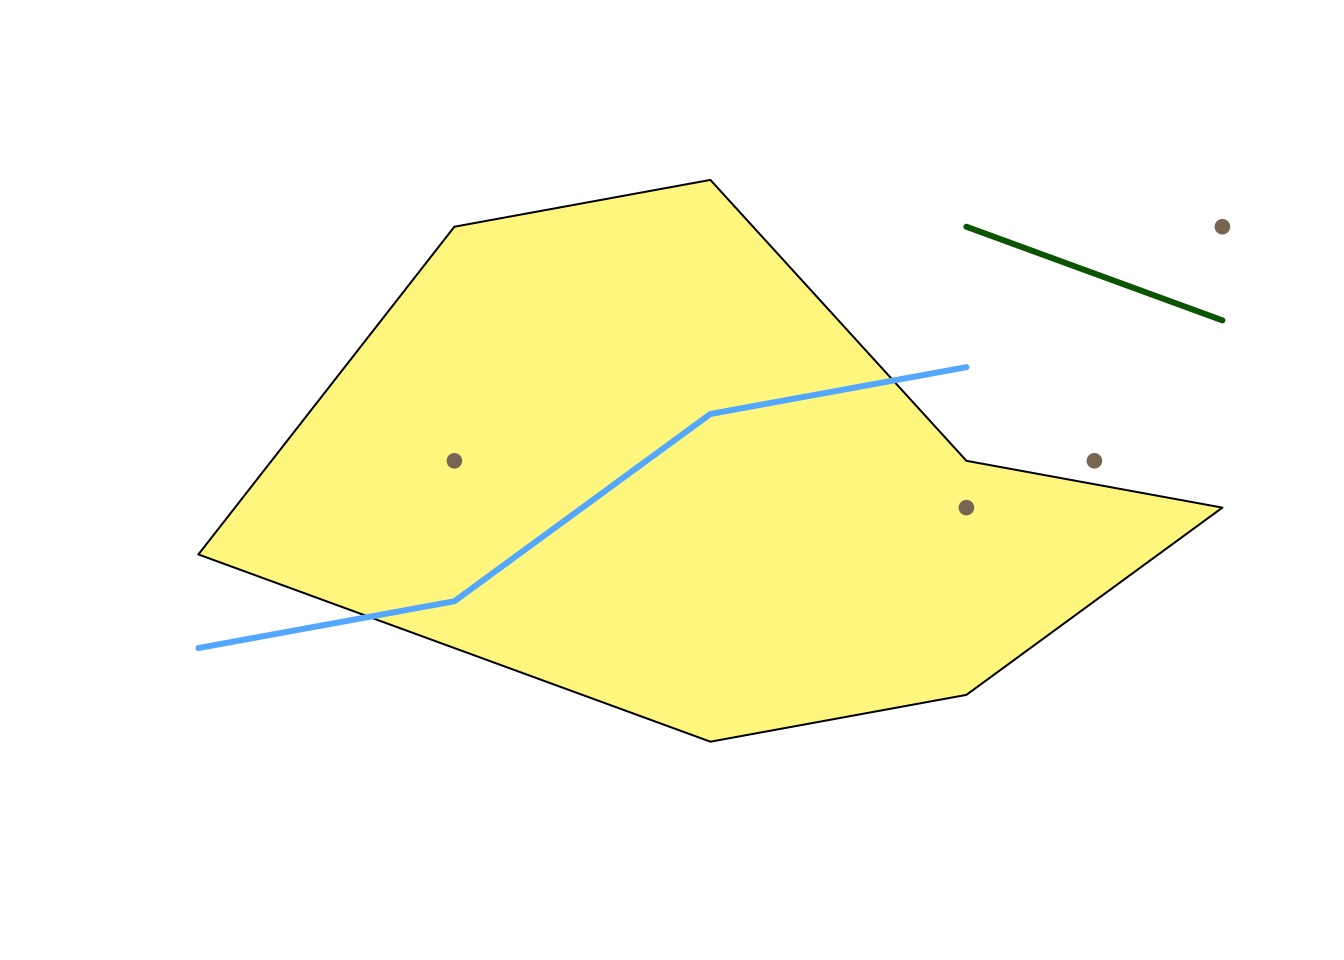
\includegraphics{R-spatial_files/figure-latex/unnamed-chunk-2-1.pdf}

\begin{quote}
Challenge

Discuss with your neighbor: What information do we need to store in
order to define points, lines, polygons in geographic space?
\end{quote}

There are currently two main approaches in R to handle geographic vector
data:

\subsection{\texorpdfstring{The \texttt{sp}
package}{The sp package}}\label{the-sp-package}

The first package to provide classes and methods for spatial data types
in R is called
\href{https://cran.r-project.org/package=sp}{\texttt{sp}}\footnote{R
  Bivand (2011)
  \href{http://geostat-course.org/system/files/monday_slides.pdf}{Introduction
  to representing spatial objects in R}}. Development of the \texttt{sp}
package began in the early 2000s in an attempt to standardize how
spatial data would be treated in R and to allow for better
interoperability between different analysis packages that use spatial
data. The package (first release on CRAN in 2005) provides classes and
methods to create \emph{points}, \emph{lines}, \emph{polygons}, and
\emph{grids} and to operate on them. About 350 of the spatial analysis
packages use the spatial data types that are implemented in \texttt{sp}
i.e.~they ``depend'' on the \texttt{sp} package and many more are
indirectly dependent.

The foundational structure for any spatial object in \texttt{sp} is the
\texttt{Spatial} class. It has two ``slots''
(\href{http://stackoverflow.com/a/4714080}{new-style S4 class objects in
R have pre-defined components called slots}):

\begin{itemize}
\item
  a \textbf{bounding box}
\item
  a \textbf{CRS class object} to define the Coordinate Reference System
\end{itemize}

This basic structure is then extended, depending on the characteristics
of the spatial object (point, line, polygon).

To build up a spatial object in \texttt{sp} we could follow these steps:

\begin{quote}
I. Create geometric objects (topology)
\end{quote}

\textbf{Points} (which may have 2 or 3 dimensions) are the most basic
spatial data objects. They are generated out of either a single
coordinate or a set of coordinates, like a two-column matrix or a
dataframe with a column for latitude and one for longitude.\\
\textbf{Lines} are generated out of \texttt{Line} objects. A
\texttt{Line} object is a spaghetti collection of 2D
coordinates\footnote{Coordinates should be of type double and will be
  promoted if not.} and is generated out of a two-column matrix or a
dataframe with a column for latitude and one for longitude. A
\texttt{Lines} object is a \textbf{list} of one or more \texttt{Line}
objects, for example all the contours at a single elevation.\\
\textbf{Polygons} are generated out of \texttt{Polygon} objects. A
\texttt{Polygon} object is a spaghetti collection of 2D coordinates with
equal first and last coordinates and is generated out of a two-column
matrix or a dataframe with a column for latitude and one for longitude.
A \texttt{Polygons} object is a \textbf{list} of one or more
\texttt{Polygon} objects, for example islands belonging to the same
country.

See here for a very simple example for how to create a \texttt{Line}
object:

\begin{Shaded}
\begin{Highlighting}[]
\NormalTok{ln1 <-}\StringTok{ }\KeywordTok{Line}\NormalTok{(}\KeywordTok{matrix}\NormalTok{(}\KeywordTok{runif}\NormalTok{(}\DecValTok{6}\NormalTok{), }\DataTypeTok{ncol=}\DecValTok{2}\NormalTok{))}
\KeywordTok{str}\NormalTok{(ln1)}
\end{Highlighting}
\end{Shaded}

\begin{verbatim}
#> Formal class 'Line' [package "sp"] with 1 slot
#>   ..@ coords: num [1:3, 1:2] 0.963 0.434 0.826 0.605 0.161 ...
\end{verbatim}

See here for a very simple example for how to create a \texttt{Lines}
object:

\begin{Shaded}
\begin{Highlighting}[]
\NormalTok{lns <-}\StringTok{ }\KeywordTok{Lines}\NormalTok{(}\KeywordTok{list}\NormalTok{(ln1), }\DataTypeTok{ID =} \KeywordTok{c}\NormalTok{(}\StringTok{"hwy1"}\NormalTok{)) }\CommentTok{# this contains just one Line!}
\KeywordTok{str}\NormalTok{(lns)}
\end{Highlighting}
\end{Shaded}

\begin{verbatim}
#> Formal class 'Lines' [package "sp"] with 2 slots
#>   ..@ Lines:List of 1
#>   .. ..$ :Formal class 'Line' [package "sp"] with 1 slot
#>   .. .. .. ..@ coords: num [1:3, 1:2] 0.963 0.434 0.826 0.605 0.161 ...
#>   ..@ ID   : chr "hwy1"
\end{verbatim}

\begin{quote}
\begin{enumerate}
\def\labelenumi{\Roman{enumi}.}
\setcounter{enumi}{1}
\tightlist
\item
  Create spatial objects \texttt{Spatial*} object (\texttt{*} stands for
  Points, Lines, or Polygons).
\end{enumerate}
\end{quote}

This step adds the bounding box (automatically) and the slot for the
Coordinate Reference System or CRS (which needs to be filled with a
value manually). \texttt{SpatialPoints} can be directly generated out of
the coordinates. \texttt{SpatialLines} and \texttt{SpatialPolygons}
objects are generated using lists of \texttt{Lines} or \texttt{Polygons}
objects respectively (more below).

See here for how to create a \texttt{SpatialLines} object:

\begin{Shaded}
\begin{Highlighting}[]
\NormalTok{sp_lns <-}\StringTok{ }\KeywordTok{SpatialLines}\NormalTok{(}\KeywordTok{list}\NormalTok{(lns))}
\KeywordTok{str}\NormalTok{(sp_lns)}
\end{Highlighting}
\end{Shaded}

\begin{verbatim}
#> Formal class 'SpatialLines' [package "sp"] with 3 slots
#>   ..@ lines      :List of 1
#>   .. ..$ :Formal class 'Lines' [package "sp"] with 2 slots
#>   .. .. .. ..@ Lines:List of 1
#>   .. .. .. .. ..$ :Formal class 'Line' [package "sp"] with 1 slot
#>   .. .. .. .. .. .. ..@ coords: num [1:3, 1:2] 0.963 0.434 0.826 0.605 0.161 ...
#>   .. .. .. ..@ ID   : chr "hwy1"
#>   ..@ bbox       : num [1:2, 1:2] 0.434 0.161 0.963 0.685
#>   .. ..- attr(*, "dimnames")=List of 2
#>   .. .. ..$ : chr [1:2] "x" "y"
#>   .. .. ..$ : chr [1:2] "min" "max"
#>   ..@ proj4string:Formal class 'CRS' [package "sp"] with 1 slot
#>   .. .. ..@ projargs: chr NA
\end{verbatim}

\begin{quote}
\begin{enumerate}
\def\labelenumi{\Roman{enumi}.}
\setcounter{enumi}{2}
\tightlist
\item
  Add attributes (\emph{Optional}:)
\end{enumerate}
\end{quote}

Add a data frame with attribute data, which will turn your
\texttt{Spatial*} object into a \texttt{Spatial*DataFrame} object. The
points in a \texttt{SpatialPoints} object may be associated with a row
of attributes to create a \texttt{SpatialPointsDataFrame} object. The
coordinates and attributes may, but do not have to be keyed to each
other using ID values.\\
\texttt{SpatialLinesDataFrame} and \texttt{SpatialPolygonsDataFrame}
objects are defined using \texttt{SpatialLines} and
\texttt{SpatialPolygons} objects and data frames. The ID fields are here
required to match the data frame row names.

See here for how to create a \texttt{SpatialLinesDataframe}:

\begin{Shaded}
\begin{Highlighting}[]
\NormalTok{dfr <-}\StringTok{ }\KeywordTok{data.frame}\NormalTok{(}\DataTypeTok{id =} \StringTok{"hwy1"}\NormalTok{, }\DataTypeTok{use =} \StringTok{"road"}\NormalTok{, }\DataTypeTok{cars_per_hour =} \DecValTok{10}\NormalTok{) }\CommentTok{# note how we use the ID from above!}
\NormalTok{sp_lns_dfr <-}\StringTok{ }\KeywordTok{SpatialLinesDataFrame}\NormalTok{(sp_lns, dfr, }\DataTypeTok{match.ID =} \StringTok{"id"}\NormalTok{)}
\KeywordTok{str}\NormalTok{(sp_lns_dfr)}
\end{Highlighting}
\end{Shaded}

\begin{verbatim}
#> Formal class 'SpatialLinesDataFrame' [package "sp"] with 4 slots
#>   ..@ data       :'data.frame':  1 obs. of  3 variables:
#>   .. ..$ id           : Factor w/ 1 level "hwy1": 1
#>   .. ..$ use          : Factor w/ 1 level "road": 1
#>   .. ..$ cars_per_hour: num 10
#>   ..@ lines      :List of 1
#>   .. ..$ :Formal class 'Lines' [package "sp"] with 2 slots
#>   .. .. .. ..@ Lines:List of 1
#>   .. .. .. .. ..$ :Formal class 'Line' [package "sp"] with 1 slot
#>   .. .. .. .. .. .. ..@ coords: num [1:3, 1:2] 0.963 0.434 0.826 0.605 0.161 ...
#>   .. .. .. ..@ ID   : chr "hwy1"
#>   ..@ bbox       : num [1:2, 1:2] 0.434 0.161 0.963 0.685
#>   .. ..- attr(*, "dimnames")=List of 2
#>   .. .. ..$ : chr [1:2] "x" "y"
#>   .. .. ..$ : chr [1:2] "min" "max"
#>   ..@ proj4string:Formal class 'CRS' [package "sp"] with 1 slot
#>   .. .. ..@ projargs: chr NA
\end{verbatim}

A number of spatial methods are available for the classes in
\texttt{sp}. Among the ones I use more frequently are:

\begin{longtable}[]{@{}ll@{}}
\toprule
\begin{minipage}[b]{0.17\columnwidth}\raggedright\strut
function\strut
\end{minipage} & \begin{minipage}[b]{0.72\columnwidth}\raggedright\strut
and what it does\strut
\end{minipage}\tabularnewline
\midrule
\endhead
\begin{minipage}[t]{0.17\columnwidth}\raggedright\strut
\texttt{bbox()}\strut
\end{minipage} & \begin{minipage}[t]{0.72\columnwidth}\raggedright\strut
returns the bounding box coordinates\strut
\end{minipage}\tabularnewline
\begin{minipage}[t]{0.17\columnwidth}\raggedright\strut
\texttt{proj4string()}\strut
\end{minipage} & \begin{minipage}[t]{0.72\columnwidth}\raggedright\strut
sets or retrieves projection attributes using the CRS object.\strut
\end{minipage}\tabularnewline
\begin{minipage}[t]{0.17\columnwidth}\raggedright\strut
\texttt{CRS()}\strut
\end{minipage} & \begin{minipage}[t]{0.72\columnwidth}\raggedright\strut
creates an object of class of coordinate reference system
arguments\strut
\end{minipage}\tabularnewline
\begin{minipage}[t]{0.17\columnwidth}\raggedright\strut
\texttt{spplot()}\strut
\end{minipage} & \begin{minipage}[t]{0.72\columnwidth}\raggedright\strut
plots a separate map of all the attributes unless specified
otherwise\strut
\end{minipage}\tabularnewline
\begin{minipage}[t]{0.17\columnwidth}\raggedright\strut
\texttt{coordinates()}\strut
\end{minipage} & \begin{minipage}[t]{0.72\columnwidth}\raggedright\strut
set or retrieve the spatial coordinates. For spatial polygons it returns
the centroids.\strut
\end{minipage}\tabularnewline
\begin{minipage}[t]{0.17\columnwidth}\raggedright\strut
\texttt{over(a,\ b)}\strut
\end{minipage} & \begin{minipage}[t]{0.72\columnwidth}\raggedright\strut
used for example to retrieve the polygon or grid indices on a set of
points\strut
\end{minipage}\tabularnewline
\begin{minipage}[t]{0.17\columnwidth}\raggedright\strut
\texttt{spsample()}\strut
\end{minipage} & \begin{minipage}[t]{0.72\columnwidth}\raggedright\strut
sampling of spatial points within the spatial extent of objects\strut
\end{minipage}\tabularnewline
\bottomrule
\end{longtable}

\subsection{\texorpdfstring{The \texttt{sf}
package}{The sf package}}\label{the-sf-package}

The second package, first released on CRAN in late October 2016, is
called
\href{https://cran.r-project.org/package=sf}{\texttt{sf}}\footnote{E.
  Pebesma \& R. Bivand
  (2016)\href{http://pebesma.staff.ifgi.de/pebesma_sfr.pdf}{Spatial data
  in R: simple features and future perspectives}}. It implements a
formal standard called
\href{https://en.wikipedia.org/wiki/Simple_Features}{``Simple
Features''} that specifies a storage and access model of spatial
geometries (point, line, polygon). A feature geometry is called simple
when it consists of points connected by straight line pieces, and does
not intersect itself. This standard has been adopted widely, not only by
spatial databases such as PostGIS, but also more recent standards such
as GeoJSON.

If you work with PostGis or GeoJSON you may have come across the
\href{https://en.wikipedia.org/wiki/Well-known_text}{WKT (well-known
text)} format, for example like these:

\begin{figure}
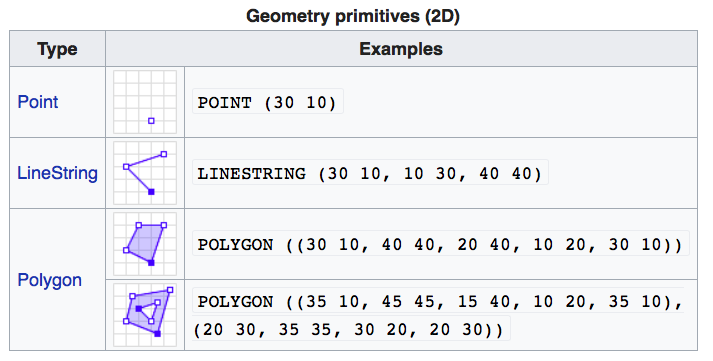
\includegraphics[width=1\linewidth]{img/wkt_primitives} \caption{Well-Known-Text Geometry primitives  (wikipedia)}\label{fig:wkt-primitives}
\end{figure}

\begin{figure}
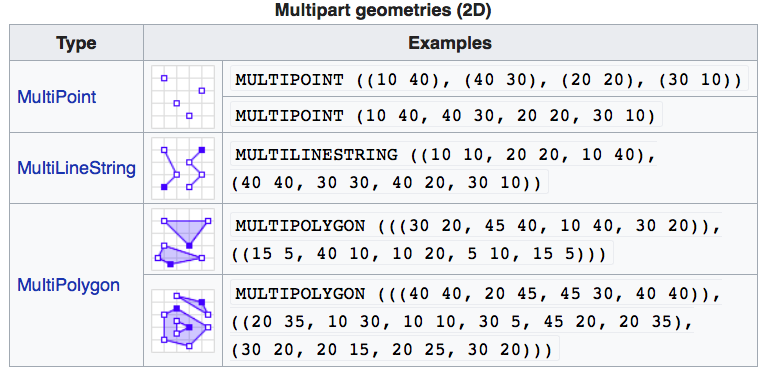
\includegraphics[width=1\linewidth]{img/wkt_multipart} \caption{Well-Known-Text Multipart geometries (wikipedia)}\label{fig:wkt-multipart}
\end{figure}

\texttt{sf} implements this standard natively in R. Data are structured
and conceptualized very differently from the \texttt{sp} approach.

In \texttt{sf} spatial objects are stored as a simple data frame with a
special column that contains the information for the geographic
coordinates. That special column is a list with the same length as the
number of rows in the data frame. Each of the individual list elements
then can be of any length needed to hold the coordinates that correspond
to an individual feature.

To create a spatial object manually the basic steps would be:

\begin{quote}
I. Create geometric objects (topology)
\end{quote}

Geometric objects (simple features) can be created from a numeric
vector, matrix or a list with the coordinates. They are called
\texttt{sfg} objects for Simple Feature Geometry.

See here for an example of how a LINESTRING \texttt{sfg} object is
created:

\begin{Shaded}
\begin{Highlighting}[]
\NormalTok{lnstr_sfg <-}\StringTok{ }\KeywordTok{st_linestring}\NormalTok{(}\KeywordTok{matrix}\NormalTok{(}\KeywordTok{runif}\NormalTok{(}\DecValTok{6}\NormalTok{), }\DataTypeTok{ncol=}\DecValTok{2}\NormalTok{)) }
\KeywordTok{class}\NormalTok{(lnstr_sfg)}
\end{Highlighting}
\end{Shaded}

\begin{verbatim}
#> [1] "XY"         "LINESTRING" "sfg"
\end{verbatim}

\begin{quote}
\begin{enumerate}
\def\labelenumi{\Roman{enumi}.}
\setcounter{enumi}{1}
\tightlist
\item
  Combine all individual single feature objects for the special column.
\end{enumerate}
\end{quote}

In order to work our way towards a data frame for all features we create
what is called an \texttt{sfc} object with all individual features,
which stands for Simple Feature Collection. The \texttt{sfc} object also
holds the bounding box and the projection information.

See here for an example of how a \texttt{sfc} object is created:

\begin{Shaded}
\begin{Highlighting}[]
\NormalTok{(lnstr_sfc <-}\StringTok{ }\KeywordTok{st_sfc}\NormalTok{(lnstr_sfg)) }\CommentTok{# just one feature here}
\end{Highlighting}
\end{Shaded}

\begin{verbatim}
#> Geometry set for 1 feature 
#> geometry type:  LINESTRING
#> dimension:      XY
#> bbox:           xmin: 0.2956037 ymin: 0.2102633 xmax: 0.9555443 ymax: 0.3919366
#> epsg (SRID):    NA
#> proj4string:    NA
\end{verbatim}

\begin{verbatim}
#> LINESTRING (0.9555443 0.3315015, 0.3090872 0.21...
\end{verbatim}

\begin{Shaded}
\begin{Highlighting}[]
\KeywordTok{class}\NormalTok{(lnstr_sfc) }
\end{Highlighting}
\end{Shaded}

\begin{verbatim}
#> [1] "sfc_LINESTRING" "sfc"
\end{verbatim}

\begin{quote}
\begin{enumerate}
\def\labelenumi{\Roman{enumi}.}
\setcounter{enumi}{2}
\tightlist
\item
  Add attributes.
\end{enumerate}
\end{quote}

We now combine the dataframe with the attributes and the simple feature
collection. See here how its done.

\begin{Shaded}
\begin{Highlighting}[]
\NormalTok{(lnstr_sf <-}\StringTok{ }\KeywordTok{st_sf}\NormalTok{(dfr , lnstr_sfc))}
\end{Highlighting}
\end{Shaded}

\begin{verbatim}
#> Simple feature collection with 1 feature and 3 fields
#> geometry type:  LINESTRING
#> dimension:      XY
#> bbox:           xmin: 0.2956037 ymin: 0.2102633 xmax: 0.9555443 ymax: 0.3919366
#> epsg (SRID):    NA
#> proj4string:    NA
#>     id  use cars_per_hour                      lnstr_sfc
#> 1 hwy1 road            10 LINESTRING (0.9555443 0.331...
\end{verbatim}

\begin{Shaded}
\begin{Highlighting}[]
\KeywordTok{class}\NormalTok{(lnstr_sf)}
\end{Highlighting}
\end{Shaded}

\begin{verbatim}
#> [1] "sf"         "data.frame"
\end{verbatim}

There are many methods available in the \texttt{sf} package, to find out
use

\begin{Shaded}
\begin{Highlighting}[]
\KeywordTok{methods}\NormalTok{(}\DataTypeTok{class=}\StringTok{"sf"}\NormalTok{)}
\end{Highlighting}
\end{Shaded}

\begin{verbatim}
#>  [1] [                     [[<-                  $<-                  
#>  [4] aggregate             as.data.frame         cbind                
#>  [7] coerce                extent                extract              
#> [10] identify              initialize            mask                 
#> [13] merge                 plot                  print                
#> [16] rasterize             rbind                 show                 
#> [19] slotsFromS3           st_agr                st_agr<-             
#> [22] st_as_sf              st_bbox               st_boundary          
#> [25] st_buffer             st_cast               st_centroid          
#> [28] st_collection_extract st_convex_hull        st_coordinates       
#> [31] st_crs                st_crs<-              st_difference        
#> [34] st_geometry           st_geometry<-         st_intersection      
#> [37] st_is                 st_line_merge         st_node              
#> [40] st_point_on_surface   st_polygonize         st_precision         
#> [43] st_segmentize         st_set_precision      st_simplify          
#> [46] st_snap               st_sym_difference     st_transform         
#> [49] st_triangulate        st_union              st_voronoi           
#> [52] st_wrap_dateline      st_write              st_zm                
#> see '?methods' for accessing help and source code
\end{verbatim}

Here are some of the other highlights of \texttt{sf} you might be
interested in:

\begin{itemize}
\item
  provides \textbf{fast} I/O, particularly relevant for large files
\item
  directly reads from and writes to spatial \textbf{databases} such as
  PostGIS
\item
  stay tuned for a new \texttt{ggplot} release that will be able to read
  and plot the \texttt{sf} format without the need of conversion to a
  data frame, like the \texttt{sp} format
\end{itemize}

Note that \texttt{sp} and \texttt{sf} are not the only way spatial
objects are conceptualized in R. Other spatial packages may use their
own class definitions for spatial data (for example \texttt{spatstat}).
Usuallly you can find functions that convert \texttt{sp} and
increasingly \texttt{sf} objects to and from these formats.

\begin{quote}
Challenge

Similarly to the example above generate a Point object in R. Use both,
the \texttt{sp} and the \texttt{sf} ``approach''.

\begin{enumerate}
\def\labelenumi{\arabic{enumi}.}
\tightlist
\item
  Create a matrix \texttt{pts} of random numbers with two columns and as
  many rows as you like. These are your points.
\item
  Create a dataframe \texttt{attrib\_df} with the same number of rows as
  your \texttt{pts} matrix and a column that holds an attribute. You can
  make up any attribute.
\item
  Use the appropriate commands and \texttt{pts} to create
\end{enumerate}

\begin{itemize}
\tightlist
\item
  a \texttt{SpatialPointsDataFrame} and
\item
  an \texttt{sf} object with a gemoetry column of class
  \texttt{sfc\_POINT}.
\end{itemize}

\begin{enumerate}
\def\labelenumi{\arabic{enumi}.}
\setcounter{enumi}{3}
\tightlist
\item
  Try to subset your spatial object using the attribute you have added
  and the way you are used to from regular data frames.
\item
  How do you determine the bounding box of your spatial object?
\end{enumerate}
\end{quote}

\section{Creating a spatial object from a lat/lon
table}\label{creating-a-spatial-object-from-a-latlon-table}

Often in your research might have a spreadsheet that contains latitude,
longitude and perhaps some attribute values. You know how to read the
spreadsheet into a data frame with \texttt{read.table} or
\texttt{read.csv}. We can then very easily convert the table into a
spatial object in R.

A \texttt{SpatialPointsDataFrame} object can be created directly from a
table by specifying which columns contain the coordinates. This can be
done in one step by using the \texttt{coordinates()} function. As
mentioned above this function can be used not only to retrieve spatial
coordinates but also to set them, which is done in R fashion with:

\begin{verbatim}
coordinates(myDataframe) <- value
\end{verbatim}

\texttt{value} can have different forms -- in this context needs to be a
character vector which specifies the data frame's columns for the
longitude and latitude (x,y) coordinates.

If we use this on a data frame it automatically converts the data frame
object into a \texttt{SpatialPointsDataFrame} object.

An \texttt{sf} object can be created from a data frame in the following
way. We take advantage of the \texttt{st\_as\_sf()} function which
converts any foreign object into an \texttt{sf} object. Similarly to
above, it requires an argument \texttt{coords}, which in the case of
point data needs to be a vector that specifies the data frame's columns
for the longitude and latitude (x,y) coordinates.

\begin{verbatim}
my_sf_object <- st_as_sf(myDataframe, coords)
\end{verbatim}

Note that \texttt{coordinates()} replaces the original data frame, while
\texttt{st\_as\_sf()} creates a new object and leaves the original data
frame untouched.

We use \texttt{read.csv()} to read \texttt{philly\_homicides.csv} into a
dataframe in R and name it \texttt{ph\_df}.

\begin{Shaded}
\begin{Highlighting}[]
\NormalTok{ph_df <-}\StringTok{ }\KeywordTok{read.csv}\NormalTok{(}\StringTok{"data/philly_homicides.csv"}\NormalTok{)}
\KeywordTok{head}\NormalTok{(ph_df)}
\end{Highlighting}
\end{Shaded}

\begin{verbatim}
#>   DC_DIST SECTOR DISPATCH_DATE DISPATCH_TIME          LOCATION_BLOCK
#> 1      22      1    2014-09-14      16:00:00 1800 BLOCK W MONTGOMERY
#> 2       1      B    2006-01-14      00:00:00   2000 BLOCK MIFFLIN ST
#> 3       1      B    2006-04-01      16:05:00   S 22ND ST /SNYDER AVE
#> 4       1      B    2006-05-10      11:13:00   2100 BLOCK MC KEAN ST
#> 5       1      E    2006-07-01      12:42:00   2100 BLOCK S HICKS ST
#> 6       1      F    2006-07-09      19:13:00   1800 BLOCK SNYDER AVE
#>   UCR_GENERAL OBJ_ID    TEXT_GENERAL_CODE   POINT_X  POINT_Y
#> 1         100      1  Homicide - Criminal -75.15680 39.98804
#> 2         100      1  Homicide - Criminal -75.17873 39.92801
#> 3         100      1  Homicide - Criminal -75.18275 39.92607
#> 4         100      1  Homicide - Criminal -75.18092 39.92704
#> 5         100      1  Homicide - Criminal -75.17204 39.92463
#> 6         100      1 Homicide - Criminal  -75.17612 39.92517
\end{verbatim}

\begin{Shaded}
\begin{Highlighting}[]
\KeywordTok{class}\NormalTok{(ph_df)}
\end{Highlighting}
\end{Shaded}

\begin{verbatim}
#> [1] "data.frame"
\end{verbatim}

We convert the \texttt{ph\_df} data frame into an \texttt{sf} object
with \texttt{st\_as\_sf()}

\begin{Shaded}
\begin{Highlighting}[]
\NormalTok{ph_sf <-}\StringTok{ }\KeywordTok{st_as_sf}\NormalTok{(ph_df , }\DataTypeTok{coords =} \KeywordTok{c}\NormalTok{(}\StringTok{"POINT_X"}\NormalTok{, }\StringTok{"POINT_Y"}\NormalTok{))}
\KeywordTok{class}\NormalTok{(ph_sf)}
\end{Highlighting}
\end{Shaded}

\begin{verbatim}
#> [1] "sf"         "data.frame"
\end{verbatim}

\begin{Shaded}
\begin{Highlighting}[]
\KeywordTok{head}\NormalTok{(ph_sf)}
\end{Highlighting}
\end{Shaded}

\begin{verbatim}
#> Simple feature collection with 6 features and 8 fields
#> geometry type:  POINT
#> dimension:      XY
#> bbox:           xmin: -75.18275 ymin: 39.92463 xmax: -75.1568 ymax: 39.98804
#> epsg (SRID):    NA
#> proj4string:    NA
#>   DC_DIST SECTOR DISPATCH_DATE DISPATCH_TIME          LOCATION_BLOCK
#> 1      22      1    2014-09-14      16:00:00 1800 BLOCK W MONTGOMERY
#> 2       1      B    2006-01-14      00:00:00   2000 BLOCK MIFFLIN ST
#> 3       1      B    2006-04-01      16:05:00   S 22ND ST /SNYDER AVE
#> 4       1      B    2006-05-10      11:13:00   2100 BLOCK MC KEAN ST
#> 5       1      E    2006-07-01      12:42:00   2100 BLOCK S HICKS ST
#> 6       1      F    2006-07-09      19:13:00   1800 BLOCK SNYDER AVE
#>   UCR_GENERAL OBJ_ID    TEXT_GENERAL_CODE                   geometry
#> 1         100      1  Homicide - Criminal  POINT (-75.1568 39.98804)
#> 2         100      1  Homicide - Criminal POINT (-75.17873 39.92801)
#> 3         100      1  Homicide - Criminal POINT (-75.18275 39.92607)
#> 4         100      1  Homicide - Criminal POINT (-75.18092 39.92704)
#> 5         100      1  Homicide - Criminal POINT (-75.17204 39.92463)
#> 6         100      1 Homicide - Criminal  POINT (-75.17612 39.92517)
\end{verbatim}

Alternatively, we convert the \texttt{ph\_df} data frame into a spatial
object with using the \texttt{coordinates} function and check with
\texttt{class(ph\_df)}again to examine which object class the table
belongs to now.

\begin{Shaded}
\begin{Highlighting}[]
\KeywordTok{coordinates}\NormalTok{(ph_df) <-}\StringTok{ }\KeywordTok{c}\NormalTok{(}\StringTok{"POINT_X"}\NormalTok{, }\StringTok{"POINT_Y"}\NormalTok{)}
\KeywordTok{class}\NormalTok{(ph_df) }\CommentTok{# !!}
\end{Highlighting}
\end{Shaded}

\begin{verbatim}
#> [1] "SpatialPointsDataFrame"
#> attr(,"package")
#> [1] "sp"
\end{verbatim}

\textbf{A brief, but important word about projection:}

Note that both the \texttt{SpatialPointsDataFrame} and the \texttt{sf}
POINTS object you just created \textbf{do not} have a projection
defined. It is ok to plot, but be aware that for any meaningful spatial
operation you will need to define a projection.

This is how it's done:

\begin{Shaded}
\begin{Highlighting}[]
\KeywordTok{is.projected}\NormalTok{(ph_df) }\CommentTok{# see if a projection is defined  }
\end{Highlighting}
\end{Shaded}

\begin{verbatim}
#> [1] NA
\end{verbatim}

\begin{Shaded}
\begin{Highlighting}[]
\KeywordTok{proj4string}\NormalTok{(ph_df) <-}\StringTok{ }\KeywordTok{CRS}\NormalTok{(}\StringTok{"+proj=longlat +ellps=WGS84 +datum=WGS84 +no_defs"}\NormalTok{) }\CommentTok{# this is WGS84}
\KeywordTok{is.projected}\NormalTok{(ph_df) }\CommentTok{# voila! hm. wait a minute..}
\end{Highlighting}
\end{Shaded}

\begin{verbatim}
#> [1] FALSE
\end{verbatim}

\begin{Shaded}
\begin{Highlighting}[]
\CommentTok{# For the `sf` object you want to use }
\KeywordTok{st_crs}\NormalTok{(ph_sf)}
\end{Highlighting}
\end{Shaded}

\begin{verbatim}
#> Coordinate Reference System: NA
\end{verbatim}

\begin{Shaded}
\begin{Highlighting}[]
\KeywordTok{st_crs}\NormalTok{(ph_sf) <-}\StringTok{ }\DecValTok{4326} \CommentTok{# we can use EPSG as numeric here}
\KeywordTok{st_crs}\NormalTok{(ph_sf)}
\end{Highlighting}
\end{Shaded}

\begin{verbatim}
#> Coordinate Reference System:
#>   EPSG: 4326 
#>   proj4string: "+proj=longlat +datum=WGS84 +no_defs"
\end{verbatim}

We will save this for later use.

\begin{Shaded}
\begin{Highlighting}[]
\KeywordTok{st_write}\NormalTok{(ph_sf, }\StringTok{"data/PhillyHomicides"}\NormalTok{, }\DataTypeTok{driver =} \StringTok{"ESRI Shapefile"}\NormalTok{)}

\CommentTok{# to save out using writeOGR from rgdal}
\CommentTok{# note that we need to save the ph_df, which we converted to sp object!}
\CommentTok{# writeOGR(ph_df, "data/PhillyHomicides", "PhillyHomcides", driver = "ESRI Shapefile")}
\end{Highlighting}
\end{Shaded}

\section{Loading shape files into R}\label{loading-shape-files-into-r}

\subsection{\texorpdfstring{How to work with
\texttt{rgdal}}{How to work with rgdal}}\label{how-to-work-with-rgdal}

In order to read spatial data into R and turn them into
\texttt{Spatial*} family objects we rely on the \texttt{rgdal} package.
It provides us direct access to the powerful \href{http://gdal.org}{GDAL
library} from within R.

We can read in and write out spatial data using:

\begin{verbatim}
readOGR() and writeOGR() (for vector)  
readGDAL() and writeGDAL() (for raster/grids)
\end{verbatim}

The parameters provided for each function vary depending on the exact
spatial file type you are reading. We will take an ESRI shapefile as an
example. A shapefile - as you know -
\href{https://en.wikipedia.org/wiki/Shapefile}{consists of various files
of the same name, but with different extensions}. They should all be in
one directory and that is what R expects.

When reading in a shapefile, \texttt{readOGR()} requires the following
two arguments:

\begin{verbatim}
datasource name (dsn)  # the path to the folder that contains the files
                       # this is a path to the folder, not a filename!
layer name (layer)     # the shapefile name WITHOUT extension
                       # this is not a path but just the name of the file!
\end{verbatim}

Setting these arguments correctly can be cause of much headache for
beginners, so let me spell it out:

\begin{itemize}
\item
  Firstly, you obviously need to know the name of shapefile.
\item
  Secondly, you need to know the name and location of the folder that
  contains all the shapefile parts.
\item
  Lastly, \texttt{readOGR} only reads the file and dumps it on your
  screen. But similarly when reading csv tables you want to actually
  work with the file, so you need to assign it to an R object.
\end{itemize}

Now let's do this.

We load the \texttt{rgdal} package and read \texttt{PhillyTotalPopHHinc}
into an object called \texttt{philly}. We can also examine the object,
for example with \texttt{summary()} or \texttt{class()}.

\begin{Shaded}
\begin{Highlighting}[]
\KeywordTok{library}\NormalTok{(rgdal)}
\NormalTok{philly_sp <-}\StringTok{ }\KeywordTok{readOGR}\NormalTok{(}\StringTok{"data/Philly/"}\NormalTok{, }\StringTok{"PhillyTotalPopHHinc"}\NormalTok{) }
\end{Highlighting}
\end{Shaded}

\begin{verbatim}
#> OGR data source with driver: ESRI Shapefile 
#> Source: "/Users/cengel/Anthro/R_Class/R_Workshops/R-spatial/data/Philly", layer: "PhillyTotalPopHHinc"
#> with 384 features
#> It has 17 fields
\end{verbatim}

\begin{Shaded}
\begin{Highlighting}[]
\CommentTok{# side note: unlike read.csv readOGR does not understand the ~ as valid element of a path. This (on Mac) will not work:}
\CommentTok{# philly <- readOGR("~/Desktop/R-data-viz/data/Philly/", "PhillyTotalPopHHinc")}
\KeywordTok{summary}\NormalTok{(philly_sp)}
\end{Highlighting}
\end{Shaded}

\begin{verbatim}
#> Object of class SpatialPolygonsDataFrame
#> Coordinates:
#>         min       max
#> x 1739496.5 1764029.7
#> y  457343.7  490544.9
#> Is projected: TRUE 
#> proj4string :
#> [+proj=aea +lat_1=29.5 +lat_2=45.5 +lat_0=37.5 +lon_0=-96 +x_0=0
#> +y_0=0 +ellps=GRS80 +units=m +no_defs]
#> Data attributes:
#>  STATEFP10 COUNTYFP10   TRACTCE10          GEOID10        NAME10   
#>  42:384    101:384    000100 :  1   42101000100:  1   1      :  1  
#>                       000200 :  1   42101000200:  1   10.01  :  1  
#>                       000300 :  1   42101000300:  1   10.02  :  1  
#>                       000401 :  1   42101000401:  1   100    :  1  
#>                       000402 :  1   42101000402:  1   101    :  1  
#>                       000500 :  1   42101000500:  1   102    :  1  
#>                       (Other):378   (Other)    :378   (Other):378  
#>               NAMELSAD10   MTFCC10    FUNCSTAT10    ALAND10        
#>  Census Tract 1    :  1   G5020:384   S:384      Min.   :   99958  
#>  Census Tract 10.01:  1                          1st Qu.:  397457  
#>  Census Tract 10.02:  1                          Median :  600362  
#>  Census Tract 100  :  1                          Mean   :  904482  
#>  Census Tract 101  :  1                          3rd Qu.:  955452  
#>  Census Tract 102  :  1                          Max.   :17228698  
#>  (Other)           :378                                            
#>     AWATER10             INTPTLAT10         INTPTLON10 
#>  Min.   :      0   +39.8798897:  1   -074.9667387:  1  
#>  1st Qu.:      0   +39.8898768:  1   -074.9702250:  1  
#>  Median :      0   +39.8904539:  1   -074.9742967:  1  
#>  Mean   :  58045   +39.8988328:  1   -074.9781805:  1  
#>  3rd Qu.:      0   +39.9024981:  1   -074.9789137:  1  
#>  Max.   :3463789   +39.9051799:  1   -074.9805151:  1  
#>                    (Other)    :378   (Other)     :378  
#>            GISJOIN      Shape_area         Shape_len        medHHinc     
#>  G4201010000100:  1   Min.   :  105512   Min.   : 1321   Min.   :  9286  
#>  G4201010000200:  1   1st Qu.:  398512   1st Qu.: 2734   1st Qu.: 24946  
#>  G4201010000300:  1   Median :  601061   Median : 3426   Median : 35365  
#>  G4201010000401:  1   Mean   :  962528   Mean   : 4239   Mean   : 38509  
#>  G4201010000402:  1   3rd Qu.:  966639   3rd Qu.: 4603   3rd Qu.: 49474  
#>  G4201010000500:  1   Max.   :20692491   Max.   :30881   Max.   :130139  
#>  (Other)       :378                                      NA's   :9       
#>     totalPop   
#>  Min.   :   0  
#>  1st Qu.:2799  
#>  Median :3914  
#>  Mean   :3974  
#>  3rd Qu.:5111  
#>  Max.   :8322  
#> 
\end{verbatim}

\begin{Shaded}
\begin{Highlighting}[]
\KeywordTok{class}\NormalTok{(philly_sp)}
\end{Highlighting}
\end{Shaded}

\begin{verbatim}
#> [1] "SpatialPolygonsDataFrame"
#> attr(,"package")
#> [1] "sp"
\end{verbatim}

Let's check out the attribute data and plot a subset of polygons with a
median household income (\texttt{medHHinc}) of over 60000 on top of the
plot of the entire city.

\begin{Shaded}
\begin{Highlighting}[]
\KeywordTok{names}\NormalTok{(philly_sp)}
\end{Highlighting}
\end{Shaded}

\begin{verbatim}
#>  [1] "STATEFP10"  "COUNTYFP10" "TRACTCE10"  "GEOID10"    "NAME10"    
#>  [6] "NAMELSAD10" "MTFCC10"    "FUNCSTAT10" "ALAND10"    "AWATER10"  
#> [11] "INTPTLAT10" "INTPTLON10" "GISJOIN"    "Shape_area" "Shape_len" 
#> [16] "medHHinc"   "totalPop"
\end{verbatim}

\begin{Shaded}
\begin{Highlighting}[]
\KeywordTok{head}\NormalTok{(philly_sp)}
\end{Highlighting}
\end{Shaded}

\begin{verbatim}
#>   STATEFP10 COUNTYFP10 TRACTCE10     GEOID10 NAME10          NAMELSAD10
#> 0        42        101    036301 42101036301 363.01 Census Tract 363.01
#> 1        42        101    036400 42101036400    364    Census Tract 364
#> 2        42        101    036600 42101036600    366    Census Tract 366
#> 3        42        101    034803 42101034803 348.03 Census Tract 348.03
#> 4        42        101    034702 42101034702 347.02 Census Tract 347.02
#> 5        42        101    036202 42101036202 362.02 Census Tract 362.02
#>   MTFCC10 FUNCSTAT10 ALAND10 AWATER10  INTPTLAT10   INTPTLON10
#> 0   G5020          S 2322732    66075 +40.0895349 -074.9667387
#> 1   G5020          S 4501110     8014 +40.1127747 -074.9789137
#> 2   G5020          S 1004313  1426278 +39.9470272 -075.1404472
#> 3   G5020          S 1271533     8021 +40.0619427 -075.0023705
#> 4   G5020          S 1016206        0 +40.0570427 -075.0283288
#> 5   G5020          S 1116115     2329 +40.0838623 -074.9781805
#>          GISJOIN Shape_area Shape_len medHHinc totalPop
#> 0 G4201010036301    2388806  6850.541    54569     3695
#> 1 G4201010036400    4509124 10567.331       NA      703
#> 2 G4201010036600    2430591  9256.983   130139     1643
#> 3 G4201010034803    1279556  4927.632    56667     4390
#> 4 G4201010034702    1016207  5919.885    69981     3807
#> 5 G4201010036202    1118443  5899.099    61513     6138
\end{verbatim}

\begin{Shaded}
\begin{Highlighting}[]
\KeywordTok{plot}\NormalTok{(philly_sp)}
\NormalTok{philly_sp_rich <-}\StringTok{ }\KeywordTok{subset}\NormalTok{(philly_sp, medHHinc }\OperatorTok{>}\StringTok{ }\DecValTok{60000}\NormalTok{)}
\KeywordTok{plot}\NormalTok{(philly_sp_rich, }\DataTypeTok{add=}\NormalTok{T, }\DataTypeTok{col=}\StringTok{"red"}\NormalTok{)}
\end{Highlighting}
\end{Shaded}

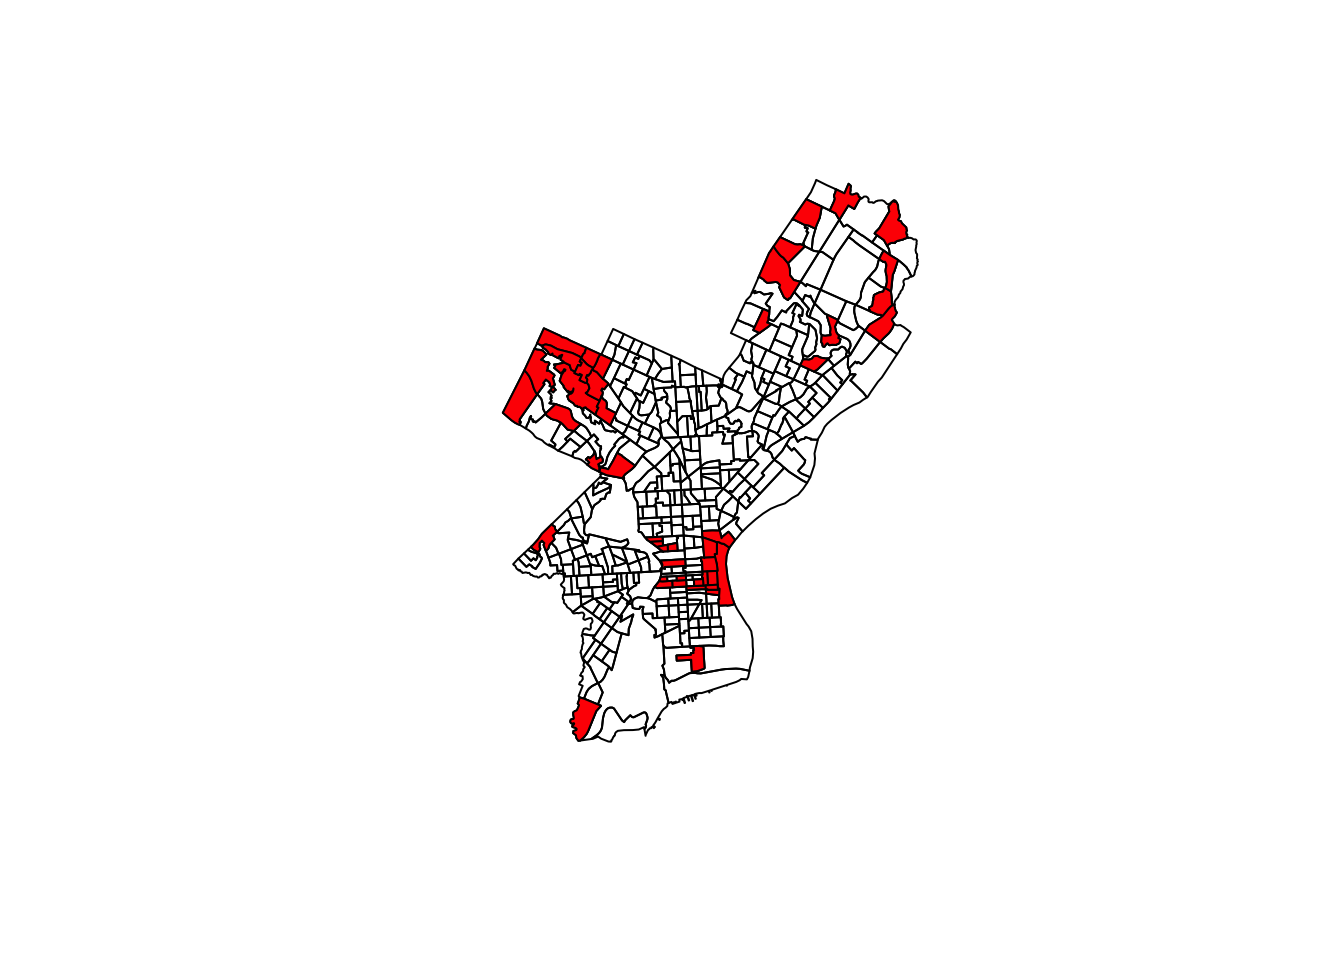
\includegraphics{R-spatial_files/figure-latex/plot-shp-sp-1.pdf}

GDAL supports over 200
\href{http://www.gdal.org/formats_list.html}{raster formats} and
\href{http://www.gdal.org/ogr_formats.html}{vector formats}. Use
\texttt{ogrDrivers()} and \texttt{gdalDrivers()} (without arguments) to
find out which formats your \texttt{rgdal} install can handle.

\subsection{\texorpdfstring{How to do this in
\texttt{sf}}{How to do this in sf}}\label{how-to-do-this-in-sf}

\texttt{sf} also relies on GDAL, but we don't need to load a separate R
library to read data in. We can use \texttt{st\_read()}, which simply
takes the path of the directory with the shapefile as argument.

So let's do the same as above using the \texttt{sf} package.

\begin{Shaded}
\begin{Highlighting}[]
\CommentTok{# read in}
\NormalTok{philly_sf <-}\StringTok{ }\KeywordTok{st_read}\NormalTok{(}\StringTok{"data/Philly/"}\NormalTok{)}
\end{Highlighting}
\end{Shaded}

\begin{verbatim}
#> Reading layer `PhillyTotalPopHHinc' from data source `/Users/cengel/Anthro/R_Class/R_Workshops/R-spatial/data/Philly' using driver `ESRI Shapefile'
#> Simple feature collection with 384 features and 17 fields
#> geometry type:  MULTIPOLYGON
#> dimension:      XY
#> bbox:           xmin: 1739497 ymin: 457343.7 xmax: 1764030 ymax: 490544.9
#> epsg (SRID):    NA
#> proj4string:    +proj=aea +lat_1=29.5 +lat_2=45.5 +lat_0=37.5 +lon_0=-96 +x_0=0 +y_0=0 +ellps=GRS80 +units=m +no_defs
\end{verbatim}

\begin{Shaded}
\begin{Highlighting}[]
\CommentTok{# take a look at what we've got}
\KeywordTok{names}\NormalTok{(philly_sf)}
\end{Highlighting}
\end{Shaded}

\begin{verbatim}
#>  [1] "STATEFP10"  "COUNTYFP10" "TRACTCE10"  "GEOID10"    "NAME10"    
#>  [6] "NAMELSAD10" "MTFCC10"    "FUNCSTAT10" "ALAND10"    "AWATER10"  
#> [11] "INTPTLAT10" "INTPTLON10" "GISJOIN"    "Shape_area" "Shape_len" 
#> [16] "medHHinc"   "totalPop"   "geometry"
\end{verbatim}

\begin{Shaded}
\begin{Highlighting}[]
\CommentTok{# note the added geometry column, as compared to:}
\KeywordTok{names}\NormalTok{(philly_sp)}
\end{Highlighting}
\end{Shaded}

\begin{verbatim}
#>  [1] "STATEFP10"  "COUNTYFP10" "TRACTCE10"  "GEOID10"    "NAME10"    
#>  [6] "NAMELSAD10" "MTFCC10"    "FUNCSTAT10" "ALAND10"    "AWATER10"  
#> [11] "INTPTLAT10" "INTPTLON10" "GISJOIN"    "Shape_area" "Shape_len" 
#> [16] "medHHinc"   "totalPop"
\end{verbatim}

\begin{Shaded}
\begin{Highlighting}[]
\CommentTok{# plot works differently here:}
\KeywordTok{plot}\NormalTok{(philly_sf)}
\end{Highlighting}
\end{Shaded}

\begin{verbatim}
#> Warning: plotting the first 10 out of 17 attributes; use max.plot = 17 to
#> plot all
\end{verbatim}

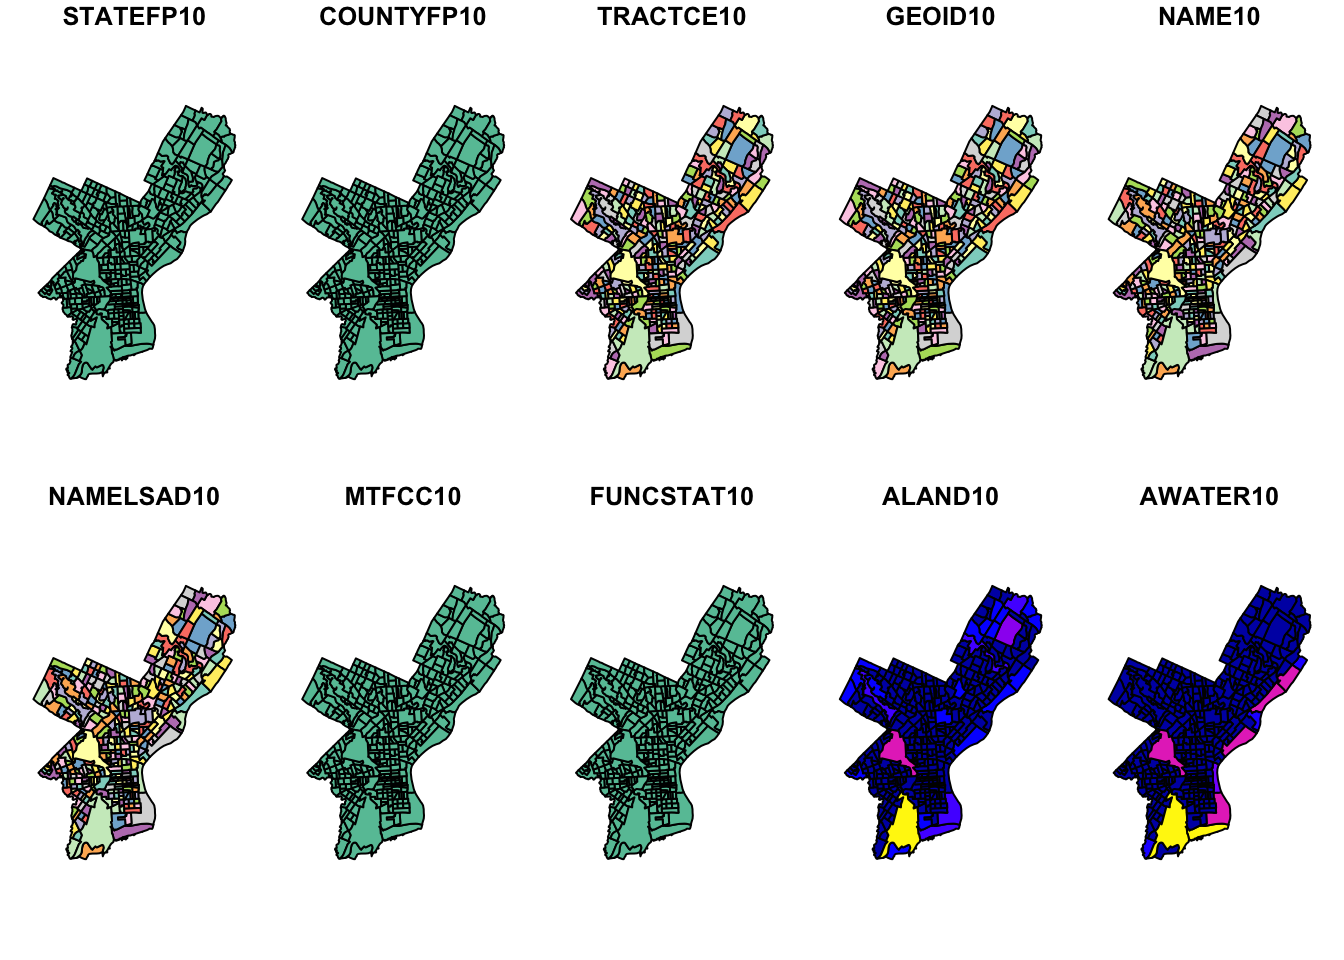
\includegraphics{R-spatial_files/figure-latex/read-shp-sf-1.pdf}

\begin{Shaded}
\begin{Highlighting}[]
\CommentTok{# to do the same as above we need to directly print the geometry column}
\KeywordTok{st_geometry}\NormalTok{(philly_sf)        }\CommentTok{# use this method to retreive geometry}
\end{Highlighting}
\end{Shaded}

\begin{verbatim}
#> Geometry set for 384 features 
#> geometry type:  MULTIPOLYGON
#> dimension:      XY
#> bbox:           xmin: 1739497 ymin: 457343.7 xmax: 1764030 ymax: 490544.9
#> epsg (SRID):    NA
#> proj4string:    +proj=aea +lat_1=29.5 +lat_2=45.5 +lat_0=37.5 +lon_0=-96 +x_0=0 +y_0=0 +ellps=GRS80 +units=m +no_defs
#> First 5 geometries:
\end{verbatim}

\begin{verbatim}
#> MULTIPOLYGON (((1763647 484837.3, 1763473 48519...
\end{verbatim}

\begin{verbatim}
#> MULTIPOLYGON (((1761348 489213.5, 1761372 48918...
\end{verbatim}

\begin{verbatim}
#> MULTIPOLYGON (((1752887 468814.9, 1752808 46863...
\end{verbatim}

\begin{verbatim}
#> MULTIPOLYGON (((1761207 482777.8, 1761634 48258...
\end{verbatim}

\begin{verbatim}
#> MULTIPOLYGON (((1759301 482266.6, 1759120 48186...
\end{verbatim}

\begin{Shaded}
\begin{Highlighting}[]
\KeywordTok{plot}\NormalTok{(}\KeywordTok{st_geometry}\NormalTok{(philly_sf))}

\CommentTok{# subset the familar way}
\NormalTok{philly_sf_rich <-}\StringTok{ }\KeywordTok{subset}\NormalTok{(philly_sf, medHHinc }\OperatorTok{>}\StringTok{ }\DecValTok{60000}\NormalTok{)}
\KeywordTok{plot}\NormalTok{(}\KeywordTok{st_geometry}\NormalTok{(philly_sf_rich), }\DataTypeTok{add=}\NormalTok{T, }\DataTypeTok{col=}\StringTok{"red"}\NormalTok{)}
\end{Highlighting}
\end{Shaded}

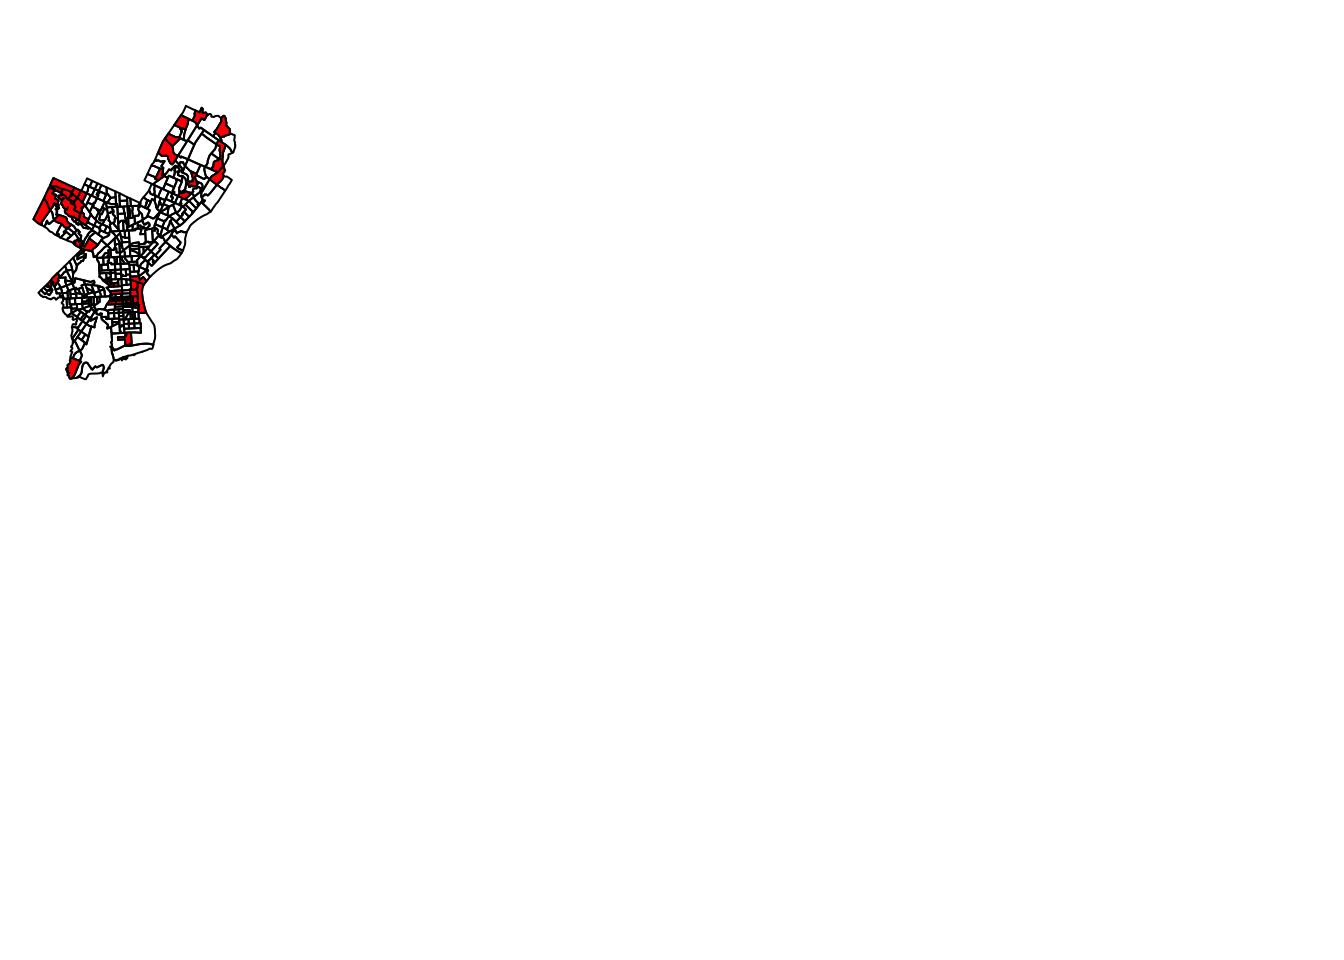
\includegraphics{R-spatial_files/figure-latex/read-shp-sf-2.pdf}

\section{Raster data in R}\label{raster-data-in-r}

Raster files, as you might know, have a much more compact data structure
than vectors. Because of their regular structure the coordinates do not
need to be recorded for each pixel or cell in the rectangular extent. A
raster is defined by:

\begin{itemize}
\tightlist
\item
  a CRS
\item
  coordinates of its origin
\item
  a distance or cell size in each direction
\item
  a dimension or numbers of cells in each direction
\item
  an array of cell values
\end{itemize}

Given this structure, coordinates for any cell can be computed and don't
need to be stored.

The \texttt{raster} package\footnote{The \texttt{geo\_join()} command
  from the
  \href{https://cran.r-project.org/web/packages/tigris/index.html}{\texttt{tigris}
  package} also provides a convenient way to merge a data frame to a
  spatial data frame.} is a major extension of spatial data classes to
access large rasters and in particular to process very large files. It
includes object classes for \texttt{RasterLayer}, \texttt{RasterStacks},
and \texttt{RasterBricks}, functions for converting among these classes,
and operators for computations on the raster data. Conversion from
\texttt{sp} type objects into \texttt{raster} type objects is possible.

If we wanted to do create a raster object from scratch we would do the
following:

\begin{Shaded}
\begin{Highlighting}[]
\CommentTok{# specify the RasterLayer with the following parameters:}
\CommentTok{# - minimum x coordinate (left border)}
\CommentTok{# - minimum y coordinate (bottom border)}
\CommentTok{# - maximum x coordinate (right border)}
\CommentTok{# - maximum y coordinate (top border)}
\CommentTok{# - resolution (cell size) in each dimension}
\NormalTok{r <-}\StringTok{ }\KeywordTok{raster}\NormalTok{(}\DataTypeTok{xmn=}\OperatorTok{-}\FloatTok{0.5}\NormalTok{, }\DataTypeTok{ymn=}\OperatorTok{-}\FloatTok{0.5}\NormalTok{, }\DataTypeTok{xmx=}\FloatTok{4.5}\NormalTok{, }\DataTypeTok{ymx=}\FloatTok{4.5}\NormalTok{, }\DataTypeTok{resolution=}\KeywordTok{c}\NormalTok{(}\DecValTok{1}\NormalTok{,}\DecValTok{1}\NormalTok{))}
\NormalTok{r}
\end{Highlighting}
\end{Shaded}

\begin{verbatim}
#> class       : RasterLayer 
#> dimensions  : 5, 5, 25  (nrow, ncol, ncell)
#> resolution  : 1, 1  (x, y)
#> extent      : -0.5, 4.5, -0.5, 4.5  (xmin, xmax, ymin, ymax)
#> coord. ref. : +proj=longlat +datum=WGS84 +ellps=WGS84 +towgs84=0,0,0
\end{verbatim}

Note that this raster object \textbf{has a CRS defined!} If the crs
argument is missing when creating the Raster object, the x coordinates
are within -360 and 360 and the y coordinates are within -90 and 90, the
WGS84 projection is used by default!

Good to know.

To add some values to the cells we could the following.

\begin{Shaded}
\begin{Highlighting}[]
\KeywordTok{class}\NormalTok{(r)}
\end{Highlighting}
\end{Shaded}

\begin{verbatim}
#> [1] "RasterLayer"
#> attr(,"package")
#> [1] "raster"
\end{verbatim}

\begin{Shaded}
\begin{Highlighting}[]
\NormalTok{r <-}\StringTok{ }\KeywordTok{setValues}\NormalTok{(r, }\KeywordTok{runif}\NormalTok{(}\DecValTok{25}\NormalTok{))}
\KeywordTok{class}\NormalTok{(r)}
\end{Highlighting}
\end{Shaded}

\begin{verbatim}
#> [1] "RasterLayer"
#> attr(,"package")
#> [1] "raster"
\end{verbatim}

\begin{Shaded}
\begin{Highlighting}[]
\KeywordTok{plot}\NormalTok{(r); }\KeywordTok{points}\NormalTok{(}\KeywordTok{coordinates}\NormalTok{(r), }\DataTypeTok{pch=}\DecValTok{3}\NormalTok{)}
\end{Highlighting}
\end{Shaded}

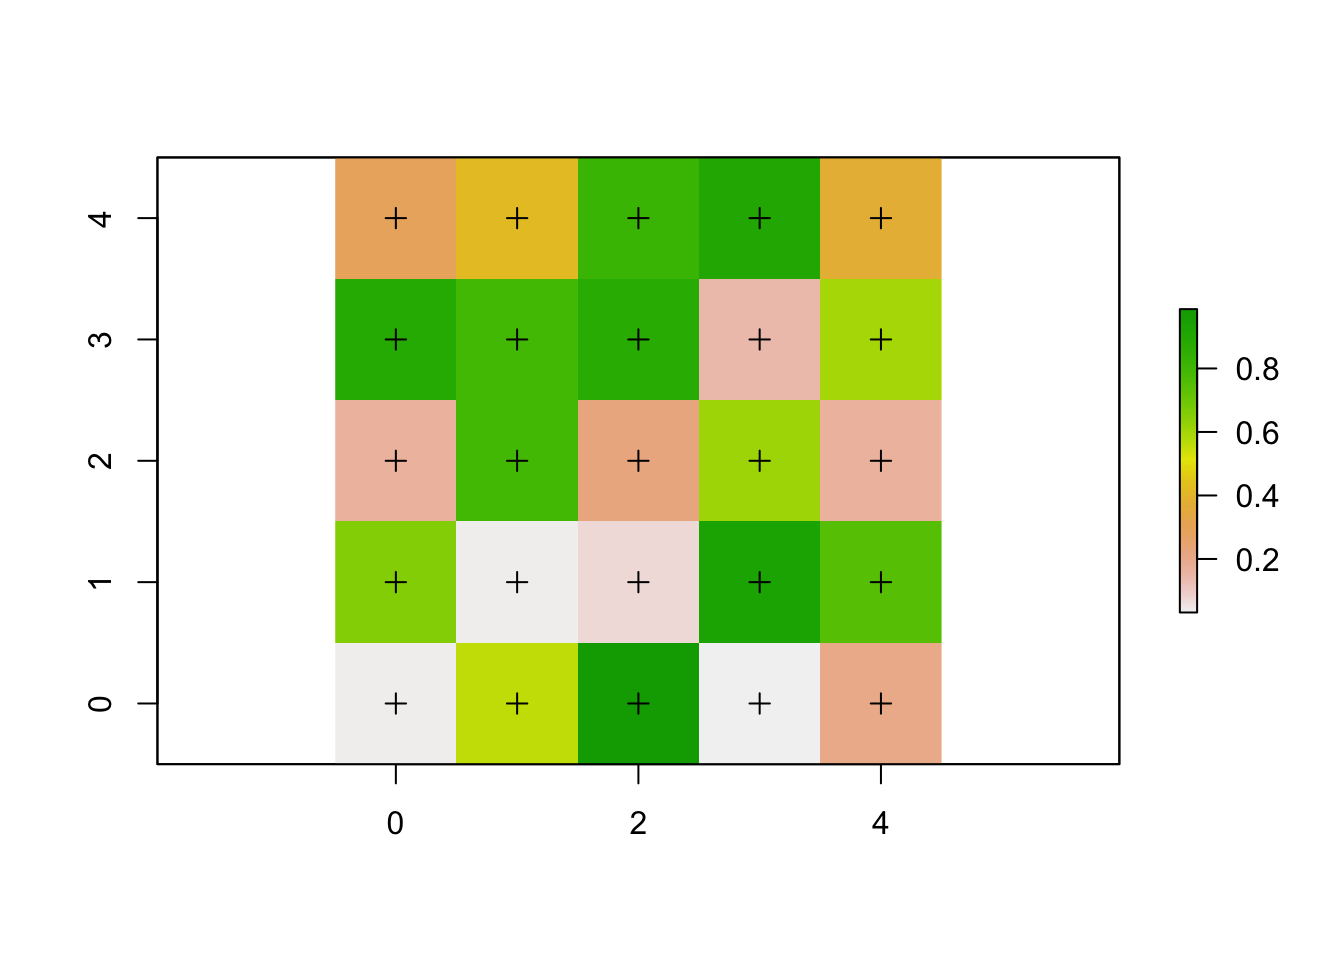
\includegraphics{R-spatial_files/figure-latex/unnamed-chunk-6-1.pdf}

(See the
\href{https://cran.r-project.org/web/packages/rasterVis/index.html}{\texttt{rasterVis}
package} for more advanced plotting of \texttt{Raster*} objects.)

RasterLayer objects can also be created from a matrix.

\begin{Shaded}
\begin{Highlighting}[]
\KeywordTok{class}\NormalTok{(volcano)}
\end{Highlighting}
\end{Shaded}

\begin{verbatim}
#> [1] "matrix"
\end{verbatim}

\begin{Shaded}
\begin{Highlighting}[]
\NormalTok{volcano.r <-}\StringTok{ }\KeywordTok{raster}\NormalTok{(volcano)}
\KeywordTok{class}\NormalTok{(volcano.r)}
\end{Highlighting}
\end{Shaded}

\begin{verbatim}
#> [1] "RasterLayer"
#> attr(,"package")
#> [1] "raster"
\end{verbatim}

And to read in a raster file we can use the \texttt{raster()} function.
This raster is generated as part of the
\href{https://www.neonscience.org/field-sites/field-sites-map/HARV}{NEON
Harvard Forest field site}.

\begin{Shaded}
\begin{Highlighting}[]
\KeywordTok{library}\NormalTok{(raster)}
\NormalTok{HARV <-}\StringTok{ }\KeywordTok{raster}\NormalTok{(}\StringTok{"data/HARV_RGB_Ortho.tif"}\NormalTok{)}
\end{Highlighting}
\end{Shaded}

Typing the name of the object will give us what's in there:

\begin{Shaded}
\begin{Highlighting}[]
\NormalTok{HARV}
\end{Highlighting}
\end{Shaded}

\begin{verbatim}
#> class       : RasterLayer 
#> band        : 1  (of  3  bands)
#> dimensions  : 2317, 3073, 7120141  (nrow, ncol, ncell)
#> resolution  : 0.25, 0.25  (x, y)
#> extent      : 731998.5, 732766.8, 4712956, 4713536  (xmin, xmax, ymin, ymax)
#> coord. ref. : +proj=utm +zone=18 +datum=WGS84 +units=m +no_defs +ellps=WGS84 +towgs84=0,0,0 
#> data source : /Users/cengel/Anthro/R_Class/R_Workshops/R-spatial/data/HARV_RGB_Ortho.tif 
#> names       : HARV_RGB_Ortho 
#> values      : 0, 255  (min, max)
\end{verbatim}

We can plot it like this:

\begin{Shaded}
\begin{Highlighting}[]
\KeywordTok{plot}\NormalTok{(HARV)}
\end{Highlighting}
\end{Shaded}

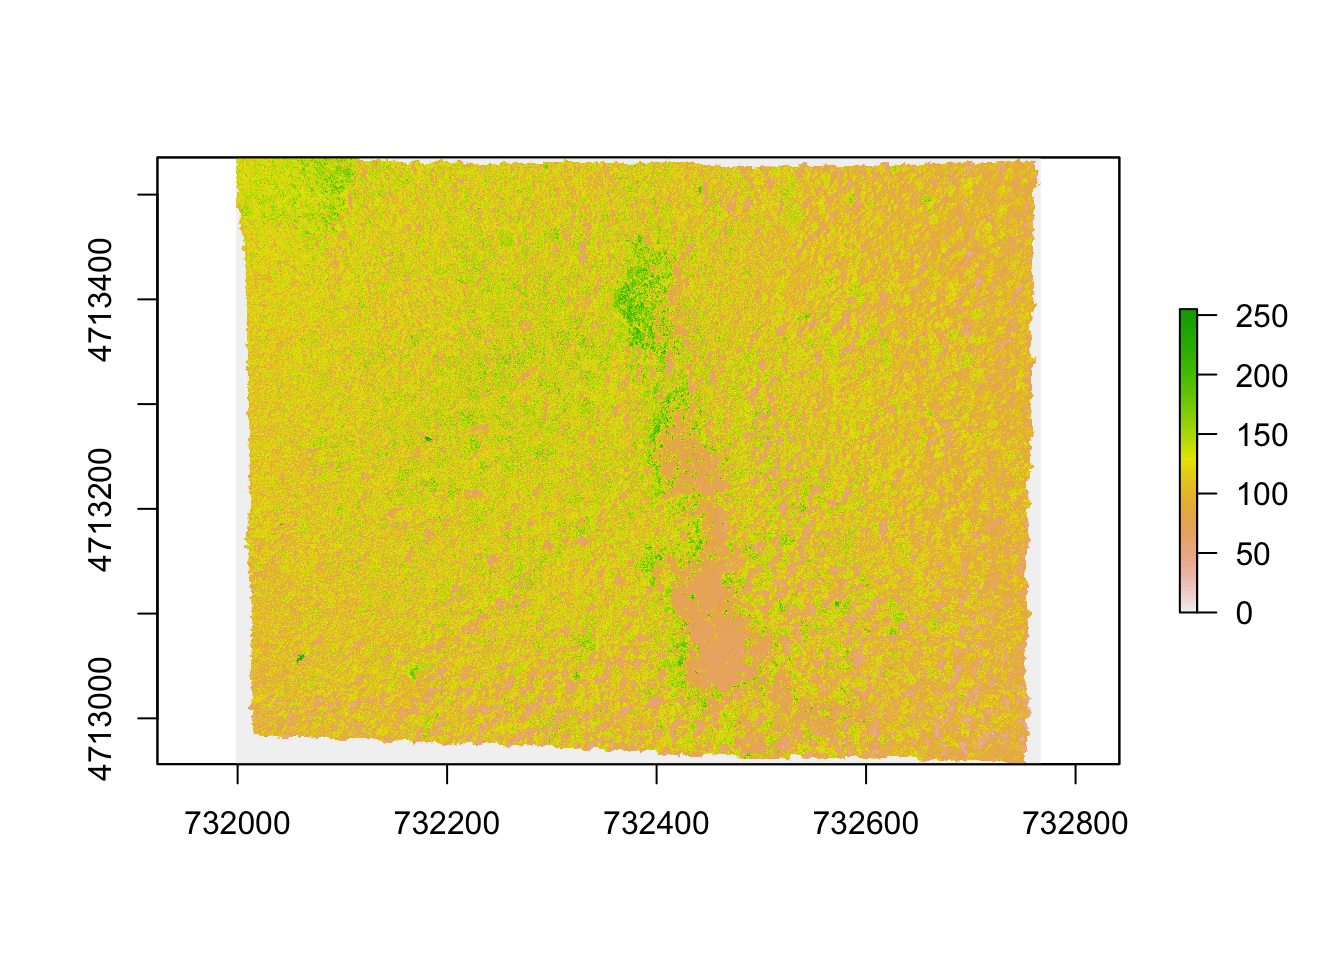
\includegraphics{R-spatial_files/figure-latex/plot-raster-1.pdf}

And we can apply functions, like this one:

\begin{Shaded}
\begin{Highlighting}[]
\KeywordTok{contour}\NormalTok{(HARV)}
\end{Highlighting}
\end{Shaded}

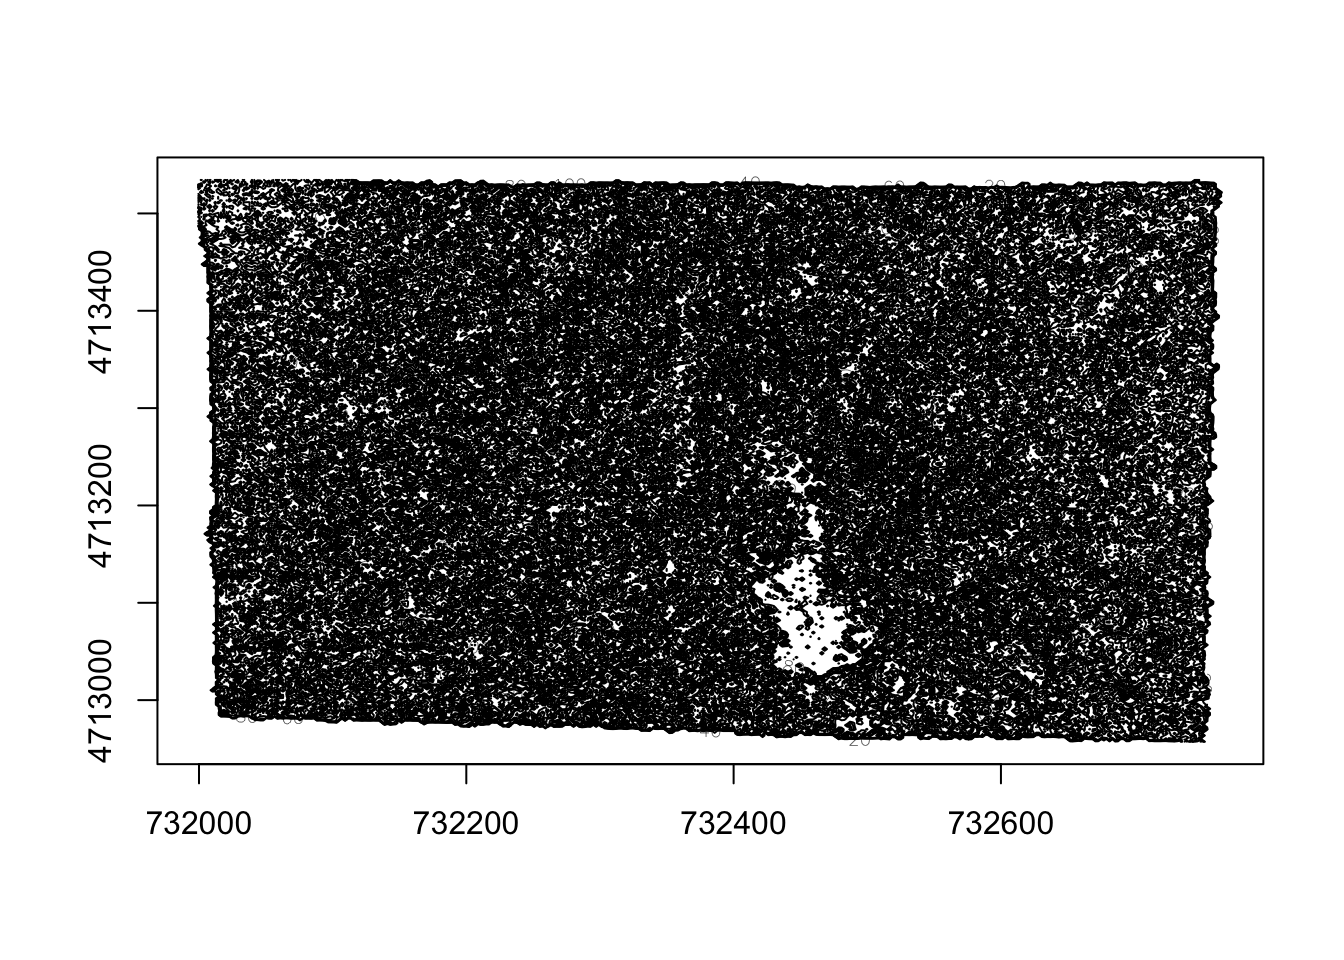
\includegraphics{R-spatial_files/figure-latex/contour-1.pdf}

We can find out about the Coordinate Reference System with this:

\begin{Shaded}
\begin{Highlighting}[]
\KeywordTok{crs}\NormalTok{(HARV)}
\end{Highlighting}
\end{Shaded}

\begin{verbatim}
#> CRS arguments:
#>  +proj=utm +zone=18 +datum=WGS84 +units=m +no_defs +ellps=WGS84
#> +towgs84=0,0,0
\end{verbatim}

See what you can do with such an object:

\begin{Shaded}
\begin{Highlighting}[]
\KeywordTok{methods}\NormalTok{(}\DataTypeTok{class=}\KeywordTok{class}\NormalTok{(HARV))}
\end{Highlighting}
\end{Shaded}

\begin{verbatim}
#>   [1] !                !=               [                [[              
#>   [5] [<-              %in%             ==               $               
#>   [9] $<-              addLayer         aggregate        all.equal       
#>  [13] area             Arith            as.array         as.data.frame   
#>  [17] as.factor        as.integer       as.list          as.logical      
#>  [21] as.matrix        as.raster        as.vector        asFactor        
#>  [25] atan2            bandnr           barplot          bbox            
#>  [29] boundaries       boxplot          brick            buffer          
#>  [33] calc             cellStats        clamp            click           
#>  [37] clump            coerce           colSums          Compare         
#>  [41] contour          coordinates      corLocal         cover           
#>  [45] crop             crosstab         cut              cv              
#>  [49] density          dim              dim<-            direction       
#>  [53] disaggregate     distance         extend           extent          
#>  [57] extract          flip             focal            freq            
#>  [61] getValues        getValuesBlock   getValuesFocal   gridDistance    
#>  [65] head             hist             image            interpolate     
#>  [69] intersect        is.factor        is.finite        is.infinite     
#>  [73] is.na            is.nan           isLonLat         KML             
#>  [77] labels           layerize         length           levels          
#>  [81] levels<-         lines            localFun         log             
#>  [85] Logic            mask             match            Math            
#>  [89] Math2            maxValue         mean             merge           
#>  [93] minValue         modal            mosaic           names           
#>  [97] names<-          ncell            ncol             nlayers         
#> [101] nrow             origin           origin<-         overlay         
#> [105] persp            plot             predict          print           
#> [109] proj4string      proj4string<-    quantile         raster          
#> [113] rasterize        readAll          readStart        readStop        
#> [117] reclassify       res              resample         RGB             
#> [121] rotate           rowSums          sampleRandom     sampleRegular   
#> [125] sampleStratified scale            select           setMinMax       
#> [129] setValues        shift            show             spplot          
#> [133] stack            stackSelect      subs             subset          
#> [137] Summary          summary          t                tail            
#> [141] text             trim             unique           update          
#> [145] values           values<-         Which            which.max       
#> [149] which.min        writeRaster      writeStart       writeStop       
#> [153] writeValues      xmax             xmin             xres            
#> [157] ymax             ymin             yres             zonal           
#> [161] zoom            
#> see '?methods' for accessing help and source code
\end{verbatim}

We can explore the distribution of values contained within our raster
using the hist() function which produces a histogram. Histograms are
often useful in identifying outliers and bad data values in our raster
data.

\begin{Shaded}
\begin{Highlighting}[]
\KeywordTok{hist}\NormalTok{(HARV)}
\end{Highlighting}
\end{Shaded}

\begin{verbatim}
#> Warning in .hist1(x, maxpixels = maxpixels, main = main, plot = plot, ...):
#> 1% of the raster cells were used. 100000 values used.
\end{verbatim}

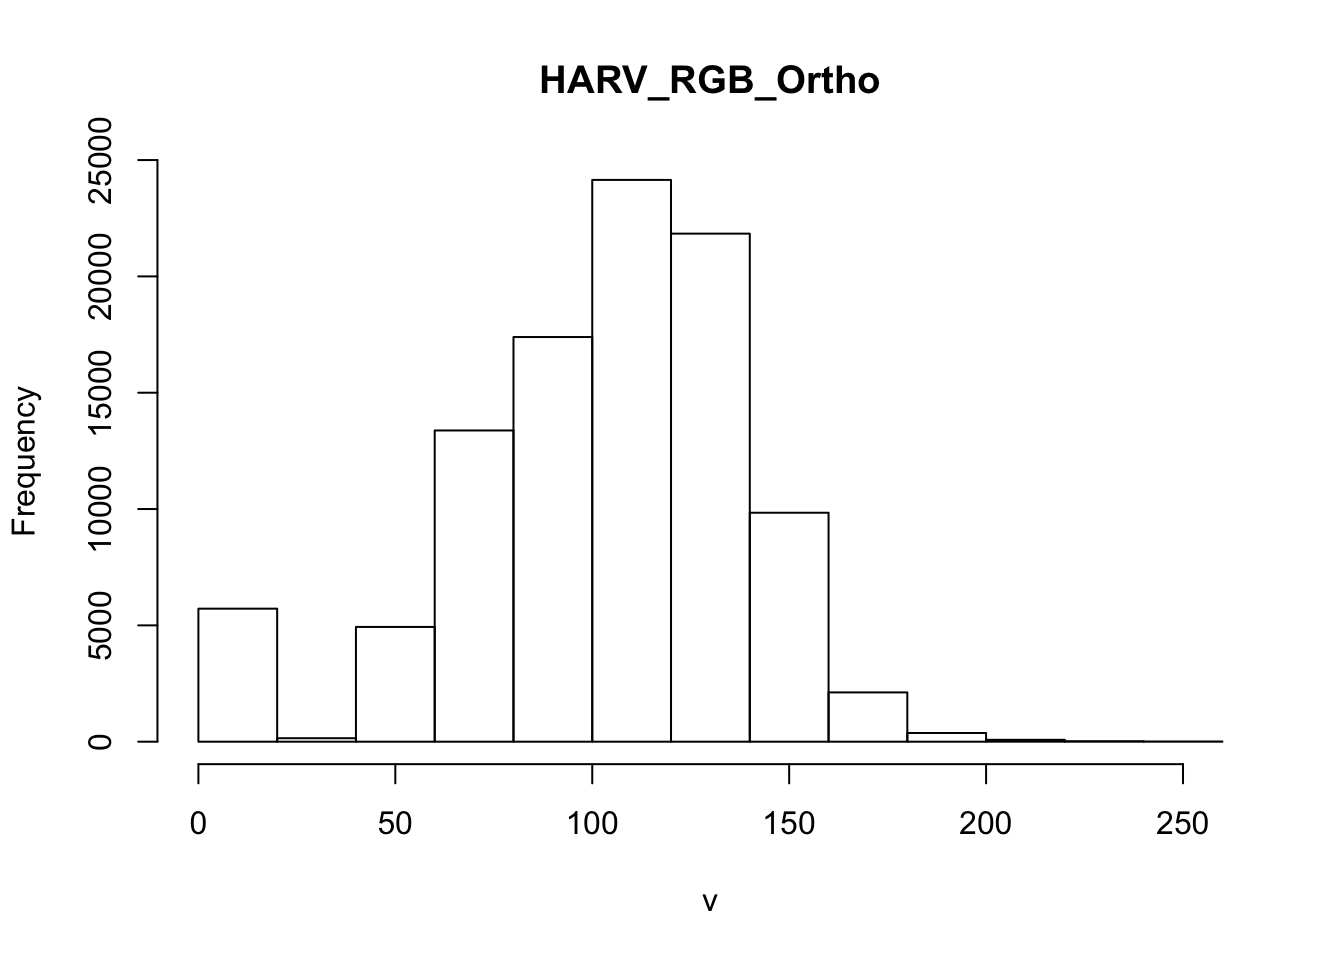
\includegraphics{R-spatial_files/figure-latex/n-hist-1.pdf}

Notice that an warning message is thrown when R creates the histogram.

This warning is caused by the default maximum pixels value of 100,000
associated with the hist function. This maximum value is to ensure
processing efficiency as our data become larger!

\begin{Shaded}
\begin{Highlighting}[]
\KeywordTok{ncell}\NormalTok{(HARV)}
\end{Highlighting}
\end{Shaded}

\begin{verbatim}
#> [1] 7120141
\end{verbatim}

\begin{Shaded}
\begin{Highlighting}[]
\KeywordTok{hist}\NormalTok{(HARV,}
     \DataTypeTok{maxpixels =} \KeywordTok{ncell}\NormalTok{(HARV))}
\end{Highlighting}
\end{Shaded}

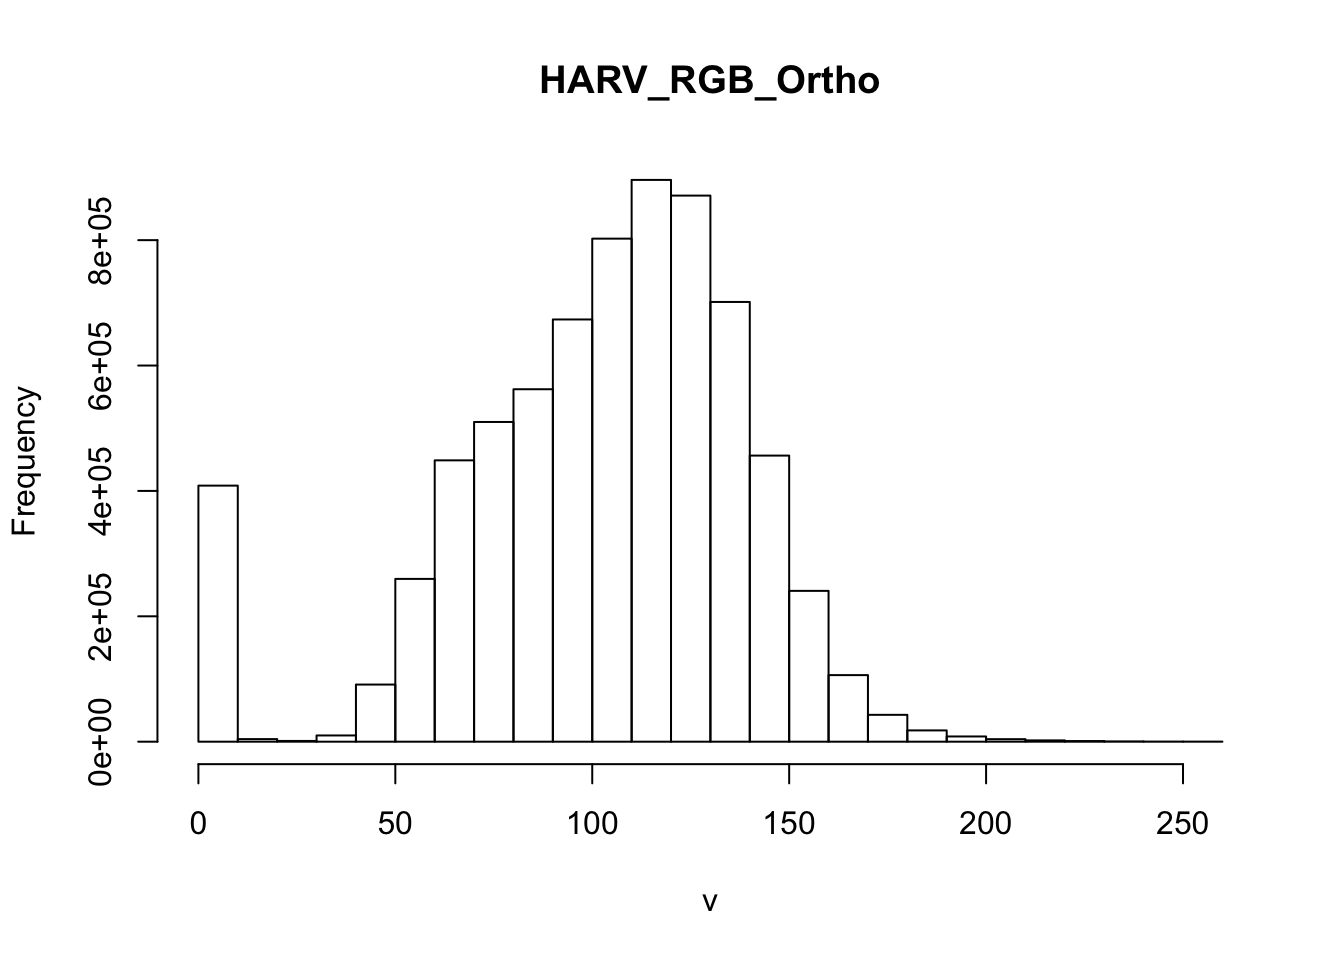
\includegraphics{R-spatial_files/figure-latex/n-hist-allvals-1.pdf}

At times it may be useful to explore raster metadata before loading them
into R. This can be done with:

\begin{verbatim}
GDALinfo("path-to-raster-here") 
\end{verbatim}

A raster dataset can contain one or more bands. We can view the number
of bands in a raster using the \texttt{nlayers()} function.

\begin{Shaded}
\begin{Highlighting}[]
\KeywordTok{nlayers}\NormalTok{(HARV)}
\end{Highlighting}
\end{Shaded}

\begin{verbatim}
#> [1] 1
\end{verbatim}

We can use the \texttt{raster()} function to import one single band from
a \emph{single} \textbf{OR} from a \emph{multi-band} raster. For
multi-band raster, we can specify which band we want to read in.

\begin{Shaded}
\begin{Highlighting}[]
\NormalTok{HARV_Band2 <-}
\StringTok{  }\KeywordTok{raster}\NormalTok{(}\StringTok{"data/HARV_RGB_Ortho.tif"}\NormalTok{, }\DataTypeTok{band =} \DecValTok{2}\NormalTok{)}

\KeywordTok{plot}\NormalTok{(HARV_Band2)}
\end{Highlighting}
\end{Shaded}

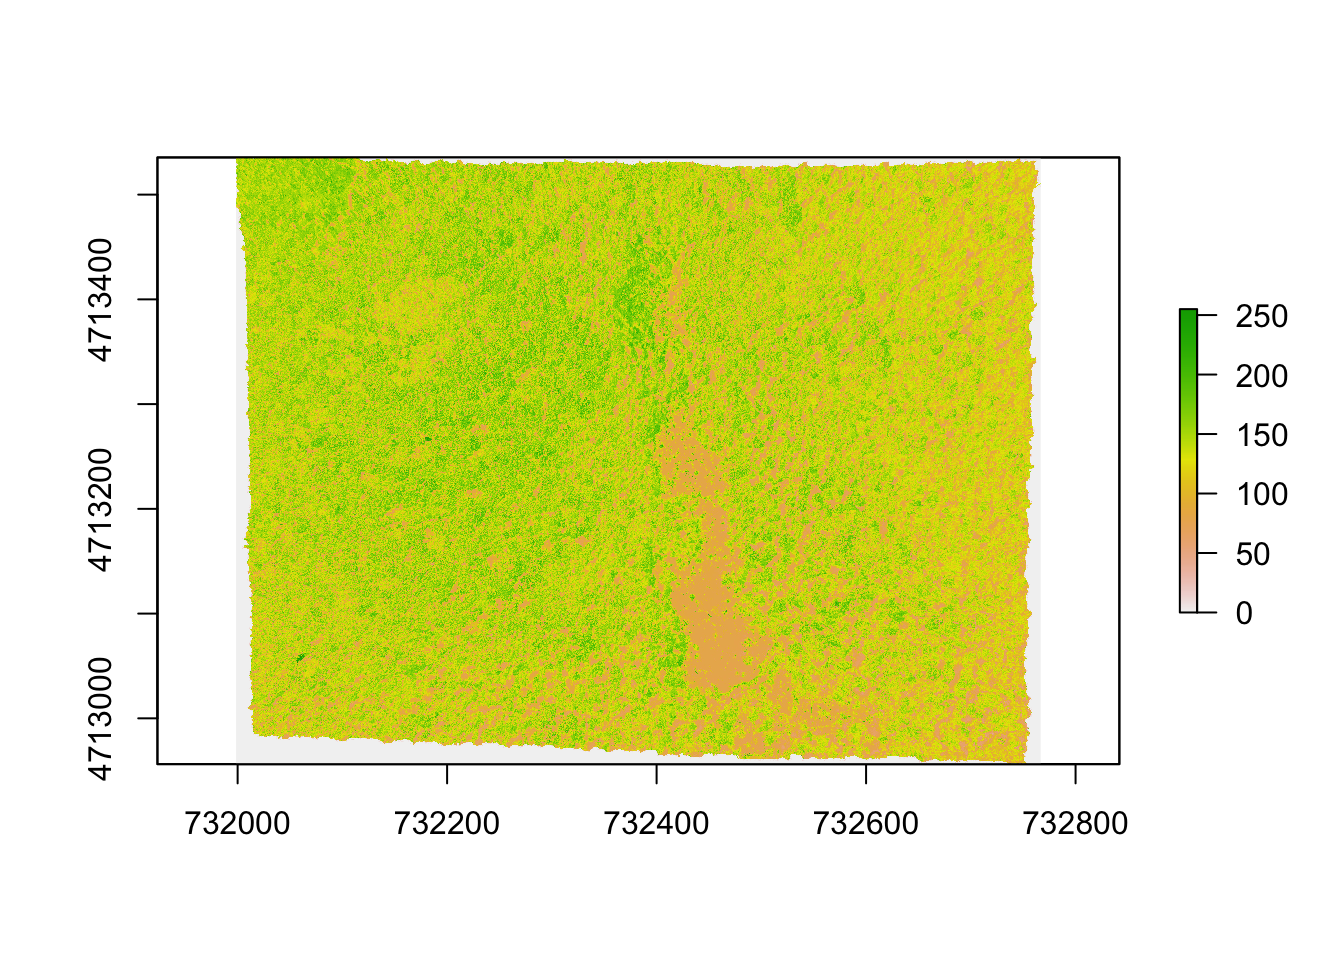
\includegraphics{R-spatial_files/figure-latex/one-multiband-1.pdf}

To bring in all bands of a multi-band raster, we use the
\texttt{stack()} function.

\begin{Shaded}
\begin{Highlighting}[]
\NormalTok{HARV_stack <-}
\StringTok{  }\KeywordTok{stack}\NormalTok{(}\StringTok{"data/HARV_RGB_Ortho.tif"}\NormalTok{)}

\CommentTok{# how many layers?}
\KeywordTok{nlayers}\NormalTok{(HARV)}
\end{Highlighting}
\end{Shaded}

\begin{verbatim}
#> [1] 1
\end{verbatim}

\begin{Shaded}
\begin{Highlighting}[]
\CommentTok{# view attributes of stack object}
\NormalTok{HARV_stack}
\end{Highlighting}
\end{Shaded}

\begin{verbatim}
#> class       : RasterStack 
#> dimensions  : 2317, 3073, 7120141, 3  (nrow, ncol, ncell, nlayers)
#> resolution  : 0.25, 0.25  (x, y)
#> extent      : 731998.5, 732766.8, 4712956, 4713536  (xmin, xmax, ymin, ymax)
#> coord. ref. : +proj=utm +zone=18 +datum=WGS84 +units=m +no_defs +ellps=WGS84 +towgs84=0,0,0 
#> names       : HARV_RGB_Ortho.1, HARV_RGB_Ortho.2, HARV_RGB_Ortho.3 
#> min values  :                0,                0,                0 
#> max values  :              255,              255,              255
\end{verbatim}

\begin{Shaded}
\begin{Highlighting}[]
\CommentTok{# what happens when we plot?}
\KeywordTok{plot}\NormalTok{(HARV_stack)}
\end{Highlighting}
\end{Shaded}

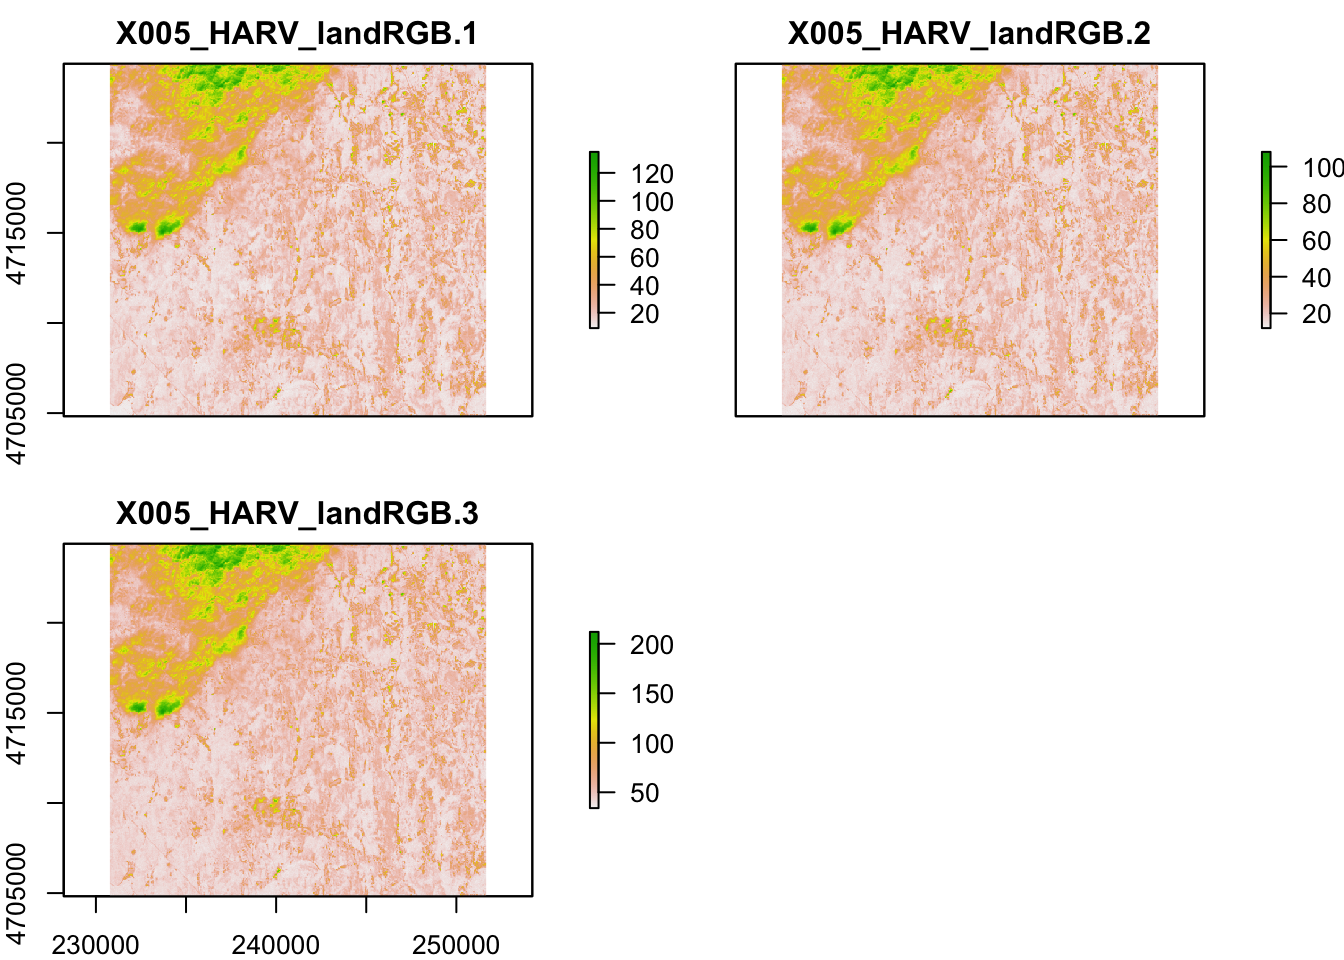
\includegraphics{R-spatial_files/figure-latex/stack-1.pdf}

\begin{Shaded}
\begin{Highlighting}[]
\CommentTok{# if we know that it is an RGB multiband raster we can plot them all in one}
\KeywordTok{plotRGB}\NormalTok{(HARV_stack)}
\end{Highlighting}
\end{Shaded}

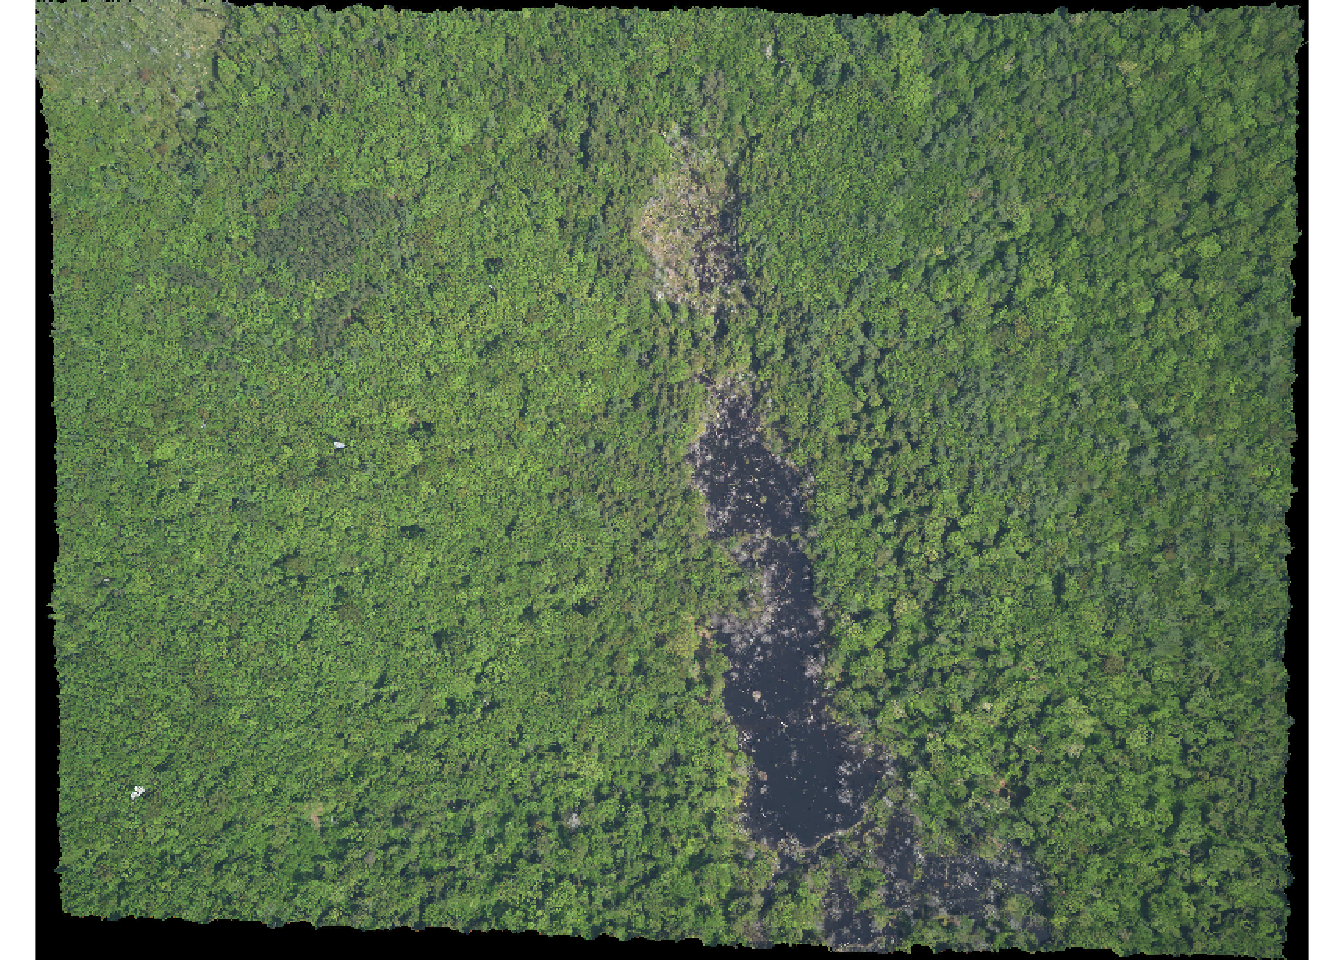
\includegraphics{R-spatial_files/figure-latex/stack-2.pdf}

\subsection{RasterStack vs RasterBrick in
R}\label{rasterstack-vs-rasterbrick-in-r}

The R \texttt{RasterStack} and \texttt{RasterBrick} object types can
both store multiple bands. However, how they store each band is
different. The bands in a \texttt{RasterStack} are stored as links to
raster data that is located somewhere on our computer. A
\texttt{RasterBrick} contains all of the objects stored within the
actual R object. Since in the \texttt{RasterBrick}, all of the bands are
stored within the actual object its object size is much larger than the
\texttt{RasterStack} object.

In most cases, we can work with a \texttt{RasterBrick} in the same way
we might work with a \texttt{RasterStack}. However, a
\texttt{RasterBrick} is often more efficient and faster to process -
which is important when working with larger files.

We can turn a \texttt{RasterStack} into a \texttt{RasterBrick} in R by
using \texttt{brick(StackName)}. Use the \texttt{object.size()} function
to compare stack and brick R objects.

\begin{Shaded}
\begin{Highlighting}[]
\KeywordTok{object.size}\NormalTok{(HARV_stack)}
\end{Highlighting}
\end{Shaded}

\begin{verbatim}
#> 41712 bytes
\end{verbatim}

\begin{Shaded}
\begin{Highlighting}[]
\NormalTok{HARV_brick <-}\StringTok{ }\KeywordTok{brick}\NormalTok{(HARV_stack)}
\KeywordTok{object.size}\NormalTok{(HARV_brick)}
\end{Highlighting}
\end{Shaded}

\begin{verbatim}
#> 170896376 bytes
\end{verbatim}

A simple grid can be built like this:

\begin{Shaded}
\begin{Highlighting}[]
\CommentTok{# specify the grid topology with the following parameters:}
\CommentTok{# - the smallest coordinates for each dimension, here: 0,0}
\CommentTok{# - cell size in each dimension, here: 1,1 }
\CommentTok{# - number of cells in each dimension, here: 5,5}
\NormalTok{gtopo <-}\StringTok{ }\KeywordTok{GridTopology}\NormalTok{(}\KeywordTok{c}\NormalTok{(}\DecValTok{0}\NormalTok{,}\DecValTok{0}\NormalTok{), }\KeywordTok{c}\NormalTok{(}\DecValTok{1}\NormalTok{,}\DecValTok{1}\NormalTok{), }\KeywordTok{c}\NormalTok{(}\DecValTok{5}\NormalTok{,}\DecValTok{5}\NormalTok{)) }\CommentTok{# create the grid}
\NormalTok{datafr <-}\StringTok{ }\KeywordTok{data.frame}\NormalTok{(}\KeywordTok{runif}\NormalTok{(}\DecValTok{25}\NormalTok{)) }\CommentTok{# make up some data}
\NormalTok{SpGdf <-}\StringTok{ }\KeywordTok{SpatialGridDataFrame}\NormalTok{(gtopo, datafr) }\CommentTok{# create the grid data frame}
\KeywordTok{summary}\NormalTok{(SpGdf)}
\end{Highlighting}
\end{Shaded}

\chapter{Spatial data manipulation in R}\label{spatialops}

\begin{quote}
Learning Objectives

\begin{itemize}
\tightlist
\item
  Join attribute data to a polygon vector file
\item
  Reproject a vector file
\item
  Select polygons of a vector by location
\end{itemize}
\end{quote}

\begin{center}\rule{0.5\linewidth}{\linethickness}\end{center}

In this section we will look at some libraries and commands that allow
us to process spatial data in R and perform a few examples of commonly
used operations.

\section{Attribute Join}\label{attribute-join}

An attribute join brings tabular data into a geographic context. It
refers to the process of joining data in tabular format to data in a
format that holds the geometries (polygon, line, or point).

If you have done attribute joins of shapefiles in GIS software like
\emph{ArcGIS} or \emph{QGis} you know that you need a \textbf{unique
identifier} in both the attribute table of the shapefile and the table
to be joined.

In order to combine a \texttt{Spatial*Dataframe} with another table
(which would be a dataframe in R) we do exactly the same. We have a
\texttt{Spatial*Dataframe}\footnote{Per the
  \href{http://www.esri.com/library/whitepapers/pdfs/shapefile.pdf}{ESRI
  specification} a shapefile always has an attribute table, so when we
  read it into R with the \texttt{readOGR} command from the \texttt{sp}
  package it automatically becomes a \texttt{Spatial*Dataframe} and the
  attribute table becomes the dataframe.} that contains the geometries
and an identifying index variable for each. We combine it with a
dataframe, that includes the same index variable with additional
variables.

\begin{figure}
\centering
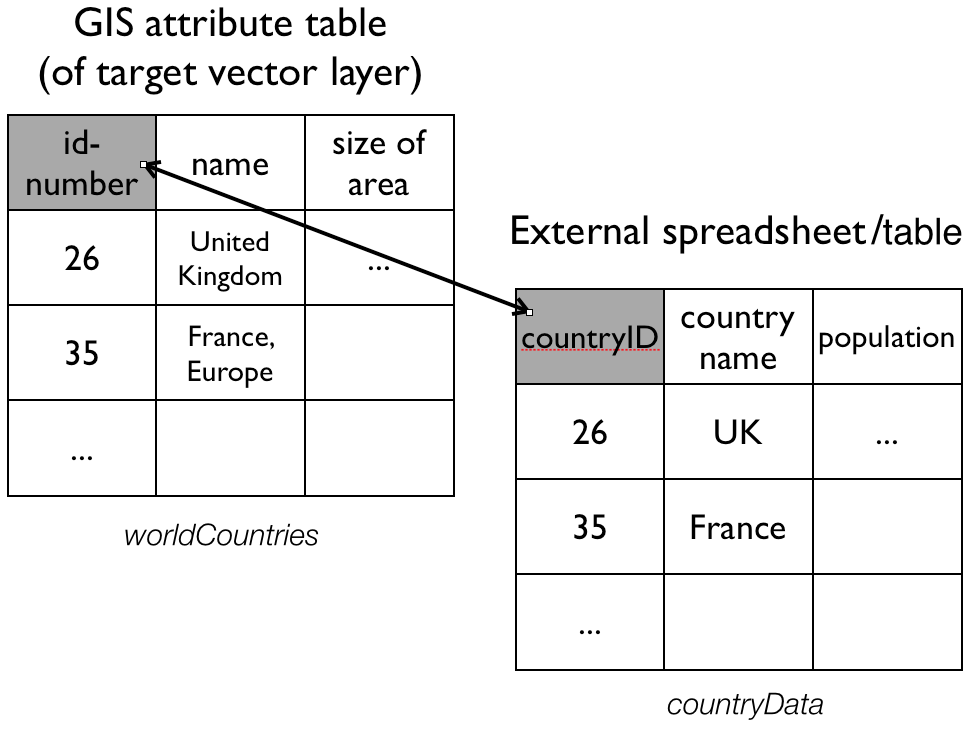
\includegraphics{img/attrJoin.png}
\caption{Attribute Join of countryData table to worldCountries using
unique ID variables}
\end{figure}

The \texttt{sp} package has a \texttt{merge} command which extends the
base \texttt{merge} command to works with \texttt{Spatial*} objects as
argument.

Assume we have:

\begin{itemize}
\tightlist
\item
  a \texttt{SpatialPolygonObject} named \emph{worldCountries}, and
\item
  a dataframe called \emph{countryData} with the attribute data to join
\end{itemize}

where:

\begin{itemize}
\tightlist
\item
  \emph{``id-number''} is the colum that contains the unique identifier
  in \emph{worldCountries}, and
\item
  \emph{``countryID''} is the column that contains the unique identifier
  in \emph{countryData}.
\end{itemize}

We would then say:

\begin{Shaded}
\begin{Highlighting}[]
\KeywordTok{library}\NormalTok{(sp) }\CommentTok{# make sure that is loaded}
\NormalTok{worldCountries <-}\StringTok{ }\KeywordTok{merge}\NormalTok{(worldCountries, countryData, }\DataTypeTok{by.x =} \StringTok{"id-number"}\NormalTok{, }\DataTypeTok{by.y =} \StringTok{"countryID"}\NormalTok{)}
\end{Highlighting}
\end{Shaded}

(You may come across alternative suggestions for joins that operate on
the data slot \texttt{@data} of the Spatial* object. While they may
work, we don't suggest them here, as good practice suggests not to use
the slot explicitly if at all possible.)

Load the CSV table \texttt{PhiladelphiaEduAttain.csv} into a dataframe
in R and name it \texttt{ph\_edu}.

\begin{Shaded}
\begin{Highlighting}[]
\NormalTok{ph_edu <-}\StringTok{ }\KeywordTok{read.csv}\NormalTok{(}\StringTok{"data/PhiladelphiaEduAttain.csv"}\NormalTok{)}
\KeywordTok{names}\NormalTok{(ph_edu)}
\end{Highlighting}
\end{Shaded}

Read the \texttt{PhillyTotalPopHHinc} shapefile into an object named
\texttt{philly\_sf}. Check out the column names of \texttt{philly\_sf}
and and of \texttt{ph\_edu} to determine which one might contain the
unique identifier for the join.

\begin{Shaded}
\begin{Highlighting}[]
\NormalTok{## sf ##}
\CommentTok{# if you need to read in again:}
\CommentTok{# philly_sf <- st_read("data/Philly/")}
\KeywordTok{names}\NormalTok{(philly_sf)}
\end{Highlighting}
\end{Shaded}

Join the \texttt{ph\_edu} data frame with \texttt{philly} using
\texttt{merge} as described above. Use the \texttt{names()} command to
see if the join was successful.

\begin{Shaded}
\begin{Highlighting}[]
\CommentTok{# this is base::merge()}
\NormalTok{philly_sf_merged <-}\StringTok{ }\KeywordTok{merge}\NormalTok{(philly_sf, ph_edu, }\DataTypeTok{by.x =} \StringTok{"GEOID10"}\NormalTok{, }\DataTypeTok{by.y =} \StringTok{"GEOID"}\NormalTok{)}
\KeywordTok{names}\NormalTok{(philly_sf_merged) }\CommentTok{# note the geometry column}
\end{Highlighting}
\end{Shaded}

\begin{verbatim}
#>  [1] "GEOID10"         "STATEFP10"       "COUNTYFP10"     
#>  [4] "TRACTCE10"       "NAME10"          "NAMELSAD10"     
#>  [7] "MTFCC10"         "FUNCSTAT10"      "ALAND10"        
#> [10] "AWATER10"        "INTPTLAT10"      "INTPTLON10"     
#> [13] "GISJOIN"         "Shape_area"      "Shape_len"      
#> [16] "medHHinc"        "totalPop"        "NAME"           
#> [19] "fem_bachelor"    "fem_doctorate"   "fem_highschool" 
#> [22] "fem_noschool"    "fem_ovr_25"      "male_bachelor"  
#> [25] "male_doctorate"  "male_highschool" "male_noschool"  
#> [28] "male_ovr_25"     "pop_ovr_25"      "geometry"
\end{verbatim}

The same with \texttt{sp}

\begin{Shaded}
\begin{Highlighting}[]
\NormalTok{## sp ##}
\CommentTok{# if you need to read in again:}
\CommentTok{# philly_sp <- readOGR("data/Philly/", "PhillyTotalPopHHinc") }

\CommentTok{# this is sp::merge()}
\NormalTok{philly_sp_merged <-}\StringTok{ }\KeywordTok{merge}\NormalTok{(philly_sp, ph_edu, }\DataTypeTok{by.x =} \StringTok{"GEOID10"}\NormalTok{, }\DataTypeTok{by.y =} \StringTok{"GEOID"}\NormalTok{)}

\KeywordTok{names}\NormalTok{(philly_sp_merged) }\CommentTok{# no geometry column here}
\end{Highlighting}
\end{Shaded}

\begin{verbatim}
#>  [1] "GEOID10"         "STATEFP10"       "COUNTYFP10"     
#>  [4] "TRACTCE10"       "NAME10"          "NAMELSAD10"     
#>  [7] "MTFCC10"         "FUNCSTAT10"      "ALAND10"        
#> [10] "AWATER10"        "INTPTLAT10"      "INTPTLON10"     
#> [13] "GISJOIN"         "Shape_area"      "Shape_len"      
#> [16] "medHHinc"        "totalPop"        "NAME"           
#> [19] "fem_bachelor"    "fem_doctorate"   "fem_highschool" 
#> [22] "fem_noschool"    "fem_ovr_25"      "male_bachelor"  
#> [25] "male_doctorate"  "male_highschool" "male_noschool"  
#> [28] "male_ovr_25"     "pop_ovr_25"
\end{verbatim}

\section{Reprojecting}\label{reprojecting}

Not unfrequently you may have to reproject spatial objects that you
perhaps have acquired from various sources and that you need to be in
the same Coordinate Reference System (CRS). The functions that do this
typically take the following two arguments:

\begin{itemize}
\tightlist
\item
  the spatial object to reproject
\item
  a CRS object with the new projection definition
\end{itemize}

You can reproject

\begin{itemize}
\tightlist
\item
  a \texttt{Spatial*} object with \texttt{spTransform()}
\item
  a \texttt{sf} object with \texttt{st\_transform()}
\item
  a \texttt{raster} object with \texttt{projectRaster()}
\end{itemize}

The perhaps trickiest part here is to determine the definition of the
projection, which needs to be a character string in
\href{http://trac.osgeo.org/proj/}{proj4} format. You can
\href{http://www.spatialreference.org}{look it up online}. For example
for \href{http://spatialreference.org/ref/epsg/wgs-84-utm-zone-33n/}{UTM
zone 33N (EPSG:32633)} the string would be:

\href{http://spatialreference.org/ref/epsg/wgs-84-utm-zone-33n/proj4js/}{\texttt{+proj=utm\ +zone=33\ +ellps=WGS84\ +datum=WGS84\ +units=m\ +no\_defs}}

You can retrieve the CRS:

\begin{itemize}
\tightlist
\item
  from an existing \texttt{Spatial*} object with \texttt{proj4string()}
\item
  from an \texttt{sf} object with \texttt{st\_crs()}
\item
  from a \texttt{raster} object with \texttt{crs()}
\end{itemize}

Let us now go back to the homicide shapefile we exported to
\texttt{"PhillyHomicides"}. Let's read it back in and transform it so it
matches the projection of the Philadelphia Census tracts. We will assign
it to a new object called \texttt{ph\_homic\_aea\_}.

First we read it in and check the CRS for both files. Then we use the
respective transformation functions to reproject.

\begin{Shaded}
\begin{Highlighting}[]
\NormalTok{## sf ##}
\NormalTok{ph_homic_sf <-}\StringTok{ }\KeywordTok{st_read}\NormalTok{(}\StringTok{"data/PhillyHomicides/"}\NormalTok{)}
\end{Highlighting}
\end{Shaded}

\begin{verbatim}
#> Reading layer `PhillyHomicides' from data source `/Users/cengel/Anthro/R_Class/R_Workshops/R-spatial/data/PhillyHomicides' using driver `ESRI Shapefile'
#> Simple feature collection with 3883 features and 8 fields
#> geometry type:  POINT
#> dimension:      XY
#> bbox:           xmin: -75.26809 ymin: 39.87503 xmax: -74.95874 ymax: 40.13086
#> epsg (SRID):    4326
#> proj4string:    +proj=longlat +datum=WGS84 +no_defs
\end{verbatim}

\begin{Shaded}
\begin{Highlighting}[]
\KeywordTok{st_crs}\NormalTok{(philly_sf)}
\end{Highlighting}
\end{Shaded}

\begin{verbatim}
#> Coordinate Reference System:
#>   No EPSG code
#>   proj4string: "+proj=aea +lat_1=29.5 +lat_2=45.5 +lat_0=37.5 +lon_0=-96 +x_0=0 +y_0=0 +ellps=GRS80 +units=m +no_defs"
\end{verbatim}

\begin{Shaded}
\begin{Highlighting}[]
\KeywordTok{st_crs}\NormalTok{(ph_homic_sf)}
\end{Highlighting}
\end{Shaded}

\begin{verbatim}
#> Coordinate Reference System:
#>   EPSG: 4326 
#>   proj4string: "+proj=longlat +datum=WGS84 +no_defs"
\end{verbatim}

\begin{Shaded}
\begin{Highlighting}[]
\NormalTok{ph_homic_aea_sf <-}\StringTok{ }\KeywordTok{st_transform}\NormalTok{(ph_homic_sf, }\KeywordTok{st_crs}\NormalTok{(philly_sf))}

\NormalTok{## sp ##}
\NormalTok{ph_homic_sp <-}\StringTok{ }\KeywordTok{readOGR}\NormalTok{(}\StringTok{"data/PhillyHomicides/"}\NormalTok{, }\StringTok{"PhillyHomicides"}\NormalTok{)}
\end{Highlighting}
\end{Shaded}

\begin{verbatim}
#> OGR data source with driver: ESRI Shapefile 
#> Source: "/Users/cengel/Anthro/R_Class/R_Workshops/R-spatial/data/PhillyHomicides", layer: "PhillyHomicides"
#> with 3883 features
#> It has 8 fields
\end{verbatim}

\begin{Shaded}
\begin{Highlighting}[]
\KeywordTok{proj4string}\NormalTok{(philly_sp)}
\end{Highlighting}
\end{Shaded}

\begin{verbatim}
#> [1] "+proj=aea +lat_1=29.5 +lat_2=45.5 +lat_0=37.5 +lon_0=-96 +x_0=0 +y_0=0 +ellps=GRS80 +units=m +no_defs"
\end{verbatim}

\begin{Shaded}
\begin{Highlighting}[]
\KeywordTok{proj4string}\NormalTok{(ph_homic_sp)}
\end{Highlighting}
\end{Shaded}

\begin{verbatim}
#> [1] "+proj=longlat +datum=WGS84 +no_defs +ellps=WGS84 +towgs84=0,0,0"
\end{verbatim}

\begin{Shaded}
\begin{Highlighting}[]
\NormalTok{ph_homic_aea_sp <-}\StringTok{ }\KeywordTok{spTransform}\NormalTok{(ph_homic_sp, }\KeywordTok{CRS}\NormalTok{(}\KeywordTok{proj4string}\NormalTok{(philly_sp)))}
\end{Highlighting}
\end{Shaded}

We can use the \texttt{range()} command from the R base package to
compare the coordinates before and after reprojection and confirm that
you actually have transformed them. \texttt{range()} simply returns the
\emph{min} and \emph{max} value of a vector of numbers that you give it.
So you can check with:

\begin{Shaded}
\begin{Highlighting}[]
\KeywordTok{range}\NormalTok{(}\KeywordTok{st_coordinates}\NormalTok{(ph_homic_aea_sf))}
\end{Highlighting}
\end{Shaded}

\begin{verbatim}
#> [1]  457489.7 1763671.8
\end{verbatim}

\begin{Shaded}
\begin{Highlighting}[]
\KeywordTok{range}\NormalTok{(}\KeywordTok{st_coordinates}\NormalTok{(ph_homic_sf))}
\end{Highlighting}
\end{Shaded}

\begin{verbatim}
#> [1] -75.26809  40.13086
\end{verbatim}

\begin{Shaded}
\begin{Highlighting}[]
\KeywordTok{range}\NormalTok{(}\KeywordTok{coordinates}\NormalTok{(ph_homic_aea_sp))}
\end{Highlighting}
\end{Shaded}

\begin{verbatim}
#> [1]  457489.7 1763671.8
\end{verbatim}

\begin{Shaded}
\begin{Highlighting}[]
\KeywordTok{range}\NormalTok{(}\KeywordTok{coordinates}\NormalTok{(ph_homic_sp))}
\end{Highlighting}
\end{Shaded}

\begin{verbatim}
#> [1] -75.26809  40.13086
\end{verbatim}

We can also compare them visually with:

\begin{Shaded}
\begin{Highlighting}[]
\KeywordTok{par}\NormalTok{(}\DataTypeTok{mfrow=}\KeywordTok{c}\NormalTok{(}\DecValTok{1}\NormalTok{,}\DecValTok{2}\NormalTok{)) }
\KeywordTok{plot}\NormalTok{(ph_homic_aea_sp, }\DataTypeTok{axes=}\OtherTok{TRUE}\NormalTok{)}
\KeywordTok{plot}\NormalTok{(ph_homic_sp, }\DataTypeTok{axes=}\OtherTok{TRUE}\NormalTok{)}
\end{Highlighting}
\end{Shaded}

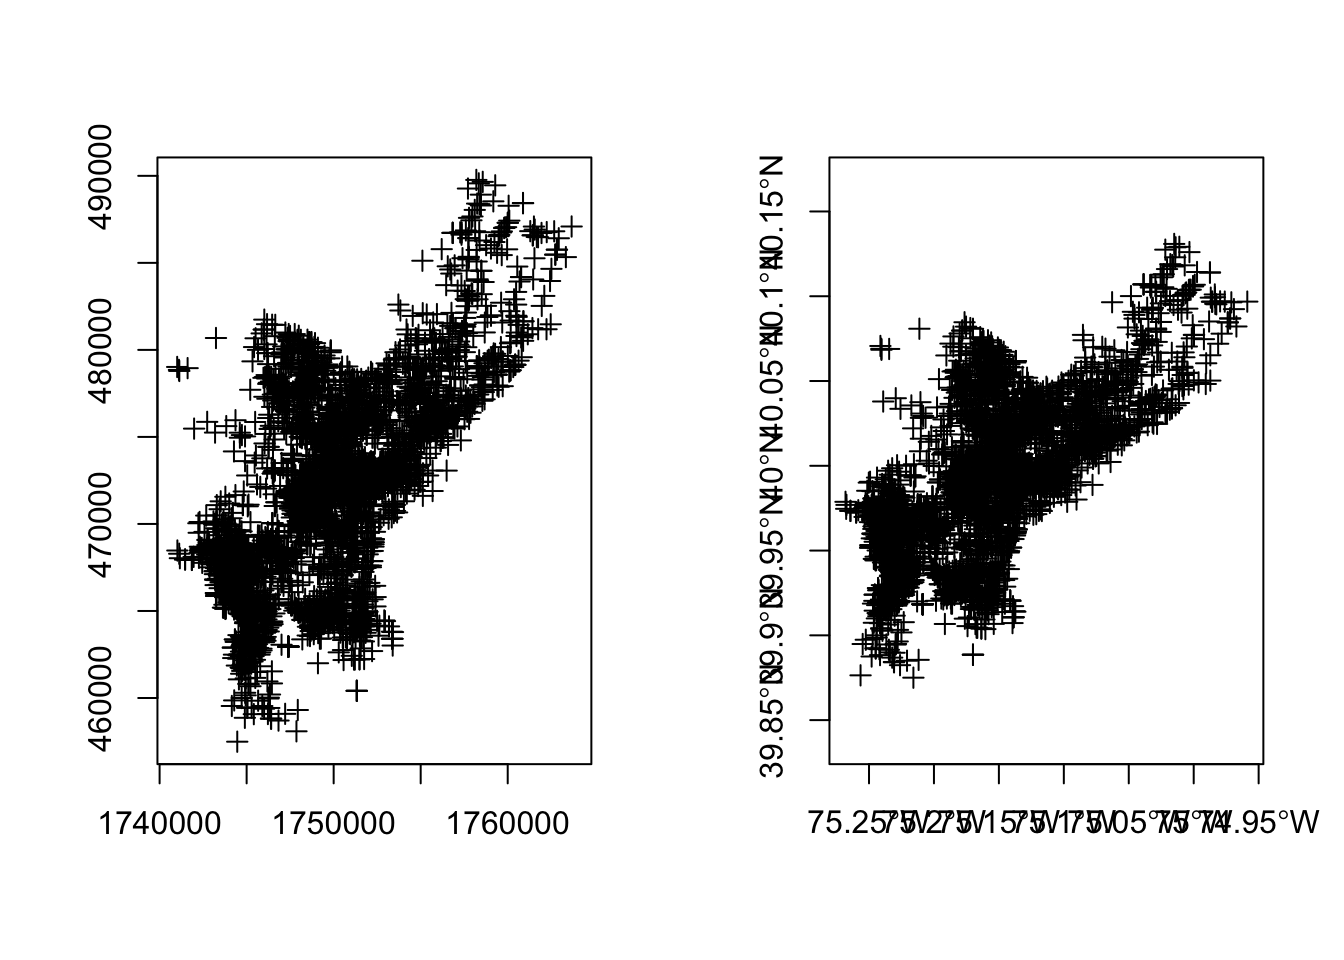
\includegraphics{R-spatial_files/figure-latex/compare-reproj-plots-1.pdf}

Here is what it would look like to reproject the HARV raster used
earlier to a WGS84 projection.

\begin{Shaded}
\begin{Highlighting}[]
\CommentTok{# if you need to load again:}
\CommentTok{#HARV <- raster("data/HARV_RGB_Ortho.tif")}
\KeywordTok{crs}\NormalTok{(HARV)}
\end{Highlighting}
\end{Shaded}

\begin{verbatim}
#> CRS arguments:
#>  +proj=utm +zone=18 +datum=WGS84 +units=m +no_defs +ellps=WGS84
#> +towgs84=0,0,0
\end{verbatim}

\begin{Shaded}
\begin{Highlighting}[]
\NormalTok{HARV.WGS84 <-}\StringTok{ }\KeywordTok{projectRaster}\NormalTok{(HARV, }\DataTypeTok{crs=}\StringTok{"+proj=longlat +ellps=WGS84 +datum=WGS84 +no_defs"}\NormalTok{)}
\KeywordTok{plot}\NormalTok{(HARV); }\KeywordTok{plot}\NormalTok{(HARV.WGS84)}
\end{Highlighting}
\end{Shaded}

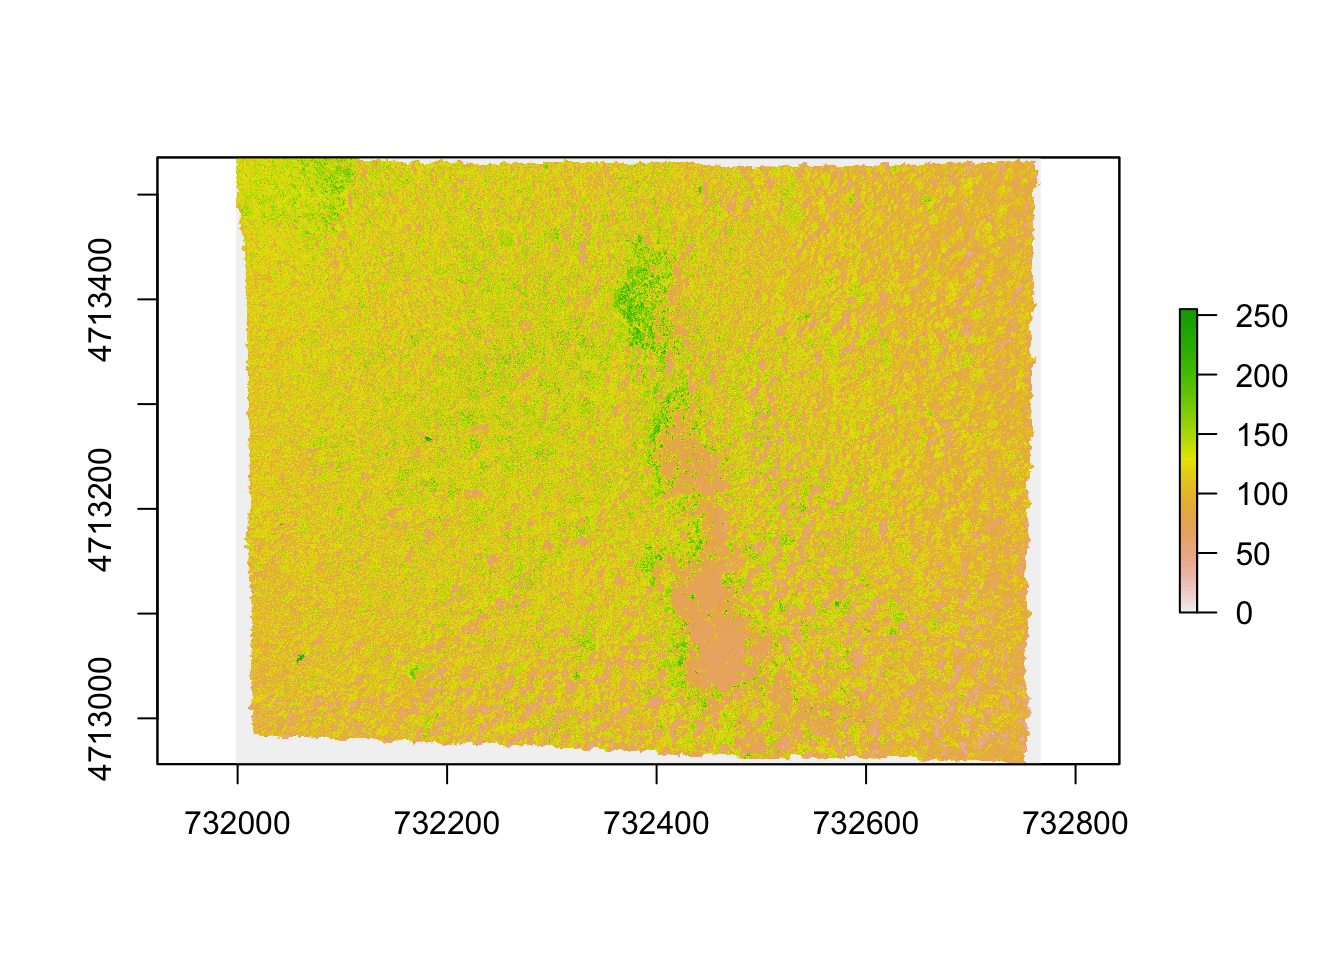
\includegraphics{R-spatial_files/figure-latex/raster-reproject-1.pdf}
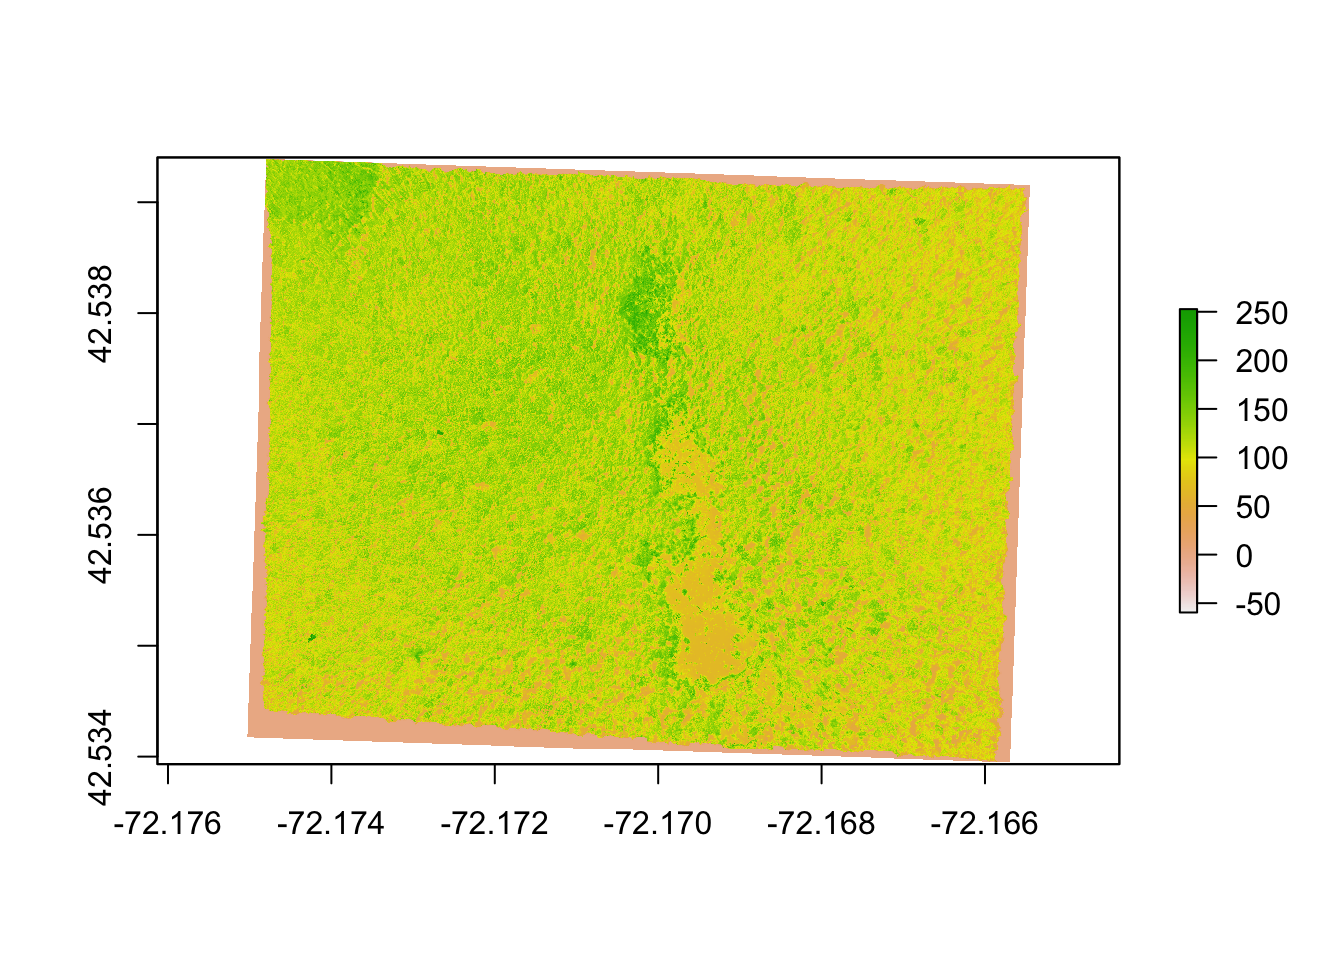
\includegraphics{R-spatial_files/figure-latex/raster-reproject-2.pdf}

\section{Points in Polygons}\label{points-in-polygons}

For the next exercise we want to calculate the density of homicides for
each census tract in Philadelphia as

\begin{verbatim}
number of homicides per census tract / area per census tract
\end{verbatim}

To achieve this this we join the points of homicide incidence to the
census tract polygon. You might be familiar with this operation from
other GIS packages.

For \texttt{sp} objects we can use the \texttt{aggregate()}
function\footnote{There is also an \texttt{aggregate()} function in the
  \texttt{stats} package that comes with the R standard install. Note
  that \texttt{sp} extends this function so it can take
  \texttt{Spatial*} objects and aggregate over the geometric features.}.
Here are the arguments that it needs:

\begin{itemize}
\tightlist
\item
  the \texttt{SpatialPointDataframe}with the homicide incidents as point
  locations,
\item
  the \texttt{SpatialPolygonDataframe} with the census tract polygons to
  aggregate on, and
\item
  an aggregate function. Since we are interested in counting the points
  (i.e.~the rows of all the points that belong to a certain polygon), we
  can use length (of the respective vectors of the aggregated data).
\end{itemize}

Let's do this.

To count homicides per census tract we use the \texttt{OBJ\_ID} field
from \texttt{ph\_homic\_aea} for homicide incidents and \texttt{philly}
polygons to aggregate on and save the result as \texttt{ph\_hom\_count}.
Use \texttt{length} as aggregate function.

\begin{Shaded}
\begin{Highlighting}[]
\NormalTok{ph_hom_count_sp <-}\StringTok{ }\KeywordTok{aggregate}\NormalTok{(}\DataTypeTok{x =}\NormalTok{ ph_homic_aea_sp[}\StringTok{"OBJ_ID"}\NormalTok{], }\DataTypeTok{by =}\NormalTok{ philly_sp, }\DataTypeTok{FUN =}\NormalTok{ length)}
\CommentTok{# make sure we understand this error message:}
\CommentTok{# aggregate(x = ph_homic_sp, by = philly_sp, FUN = length) }
\end{Highlighting}
\end{Shaded}

Now let us investigate the object we created.

\begin{Shaded}
\begin{Highlighting}[]
\KeywordTok{class}\NormalTok{(ph_hom_count_sp)}
\end{Highlighting}
\end{Shaded}

\begin{verbatim}
#> [1] "SpatialPolygonsDataFrame"
#> attr(,"package")
#> [1] "sp"
\end{verbatim}

\begin{Shaded}
\begin{Highlighting}[]
\KeywordTok{names}\NormalTok{(ph_hom_count_sp)}
\end{Highlighting}
\end{Shaded}

\begin{verbatim}
#> [1] "OBJ_ID"
\end{verbatim}

\begin{Shaded}
\begin{Highlighting}[]
\KeywordTok{head}\NormalTok{(ph_hom_count_sp)}
\end{Highlighting}
\end{Shaded}

\begin{verbatim}
#>   OBJ_ID
#> 0      2
#> 1      3
#> 2     11
#> 3      3
#> 4      4
#> 5      5
\end{verbatim}

Now we can calculate the density of homicides in Philadelphia,
normalized over the area for each census tract.

We use \texttt{gArea()} from the \texttt{rgeos} library. \texttt{gArea},
when given a \texttt{SpatialPolygon}, calculates the size of the area
covered. If we need that calculation for each polygon, we set
\texttt{byid\ =\ TRUE}. Units are in map units.

\begin{Shaded}
\begin{Highlighting}[]
\KeywordTok{library}\NormalTok{(rgeos)}
\CommentTok{# we multiply by by 1000000 to get sq km.}
\NormalTok{ph_hom_count_sp}\OperatorTok{$}\NormalTok{homic_dens <-}\StringTok{ }\FloatTok{1e6} \OperatorTok{*}\StringTok{ }\NormalTok{(ph_hom_count_sp}\OperatorTok{$}\NormalTok{OBJ_ID}\OperatorTok{/}\KeywordTok{gArea}\NormalTok{(ph_hom_count_sp, }\DataTypeTok{byid =} \OtherTok{FALSE}\NormalTok{))}

\KeywordTok{hist}\NormalTok{(ph_hom_count_sp}\OperatorTok{$}\NormalTok{homic_dens)}
\end{Highlighting}
\end{Shaded}

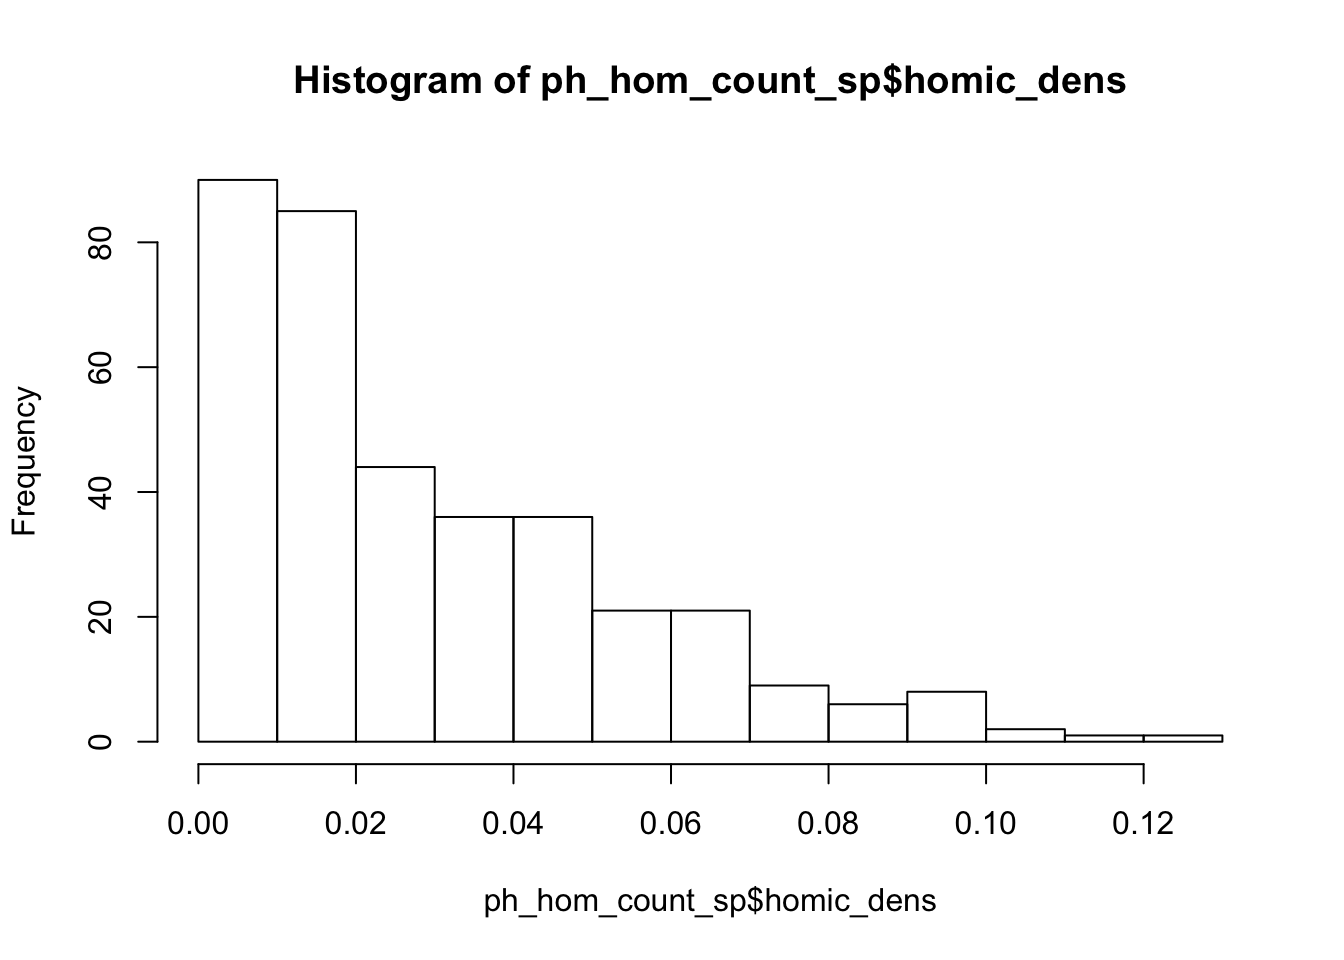
\includegraphics{R-spatial_files/figure-latex/sp-crime-rate-1.pdf}

We will write it out for later. (Note that this will produce an error if
the file already exists. You can force it to write out with the option
\texttt{overwrite\_layer\ =\ TRUE})

\begin{Shaded}
\begin{Highlighting}[]
\KeywordTok{writeOGR}\NormalTok{(ph_hom_count_sp, }\StringTok{"data/PhillyCrimerate"}\NormalTok{, }\StringTok{"PhillyCrimerate"}\NormalTok{, }\DataTypeTok{driver =} \StringTok{"ESRI Shapefile"}\NormalTok{)}
\end{Highlighting}
\end{Shaded}

There might be other instances where we don't want to aggregate, but
might only want to know which polygon a point falls into. In that case
we can use \texttt{over()}. In fact, the \texttt{aggregate()} function
used above makes use of \texttt{over()}. See
\url{https://cran.r-project.org/web/packages/sp/vignettes/over.pdf} for
more details on the over-methods. \texttt{point.in.poly()} from the
\href{https://cran.r-project.org/package=spatialEco}{\texttt{spatialEco}}
package intersects point and polygons and adds polygon attributes to
points. There is also \texttt{point.in.polygon()} from the \texttt{sp}
package which tests if a point or set of points fall in a given polygon.

For \texttt{sf} objects we need to add one more step. We first use
\texttt{st\_within()} to determine which polygon a points falls into. We
can then use the result to aggregate.

\begin{quote}
\begin{quote}
\begin{quote}
Need to add this
\end{quote}
\end{quote}
\end{quote}

\section{Select Polygons by Location}\label{select-polygons-by-location}

For the next example our goal is to select all Philadelphia census
tracts within a range of 2 kilometers from the city center.

\begin{quote}
Think about this for a moment -- what might be the steps you'd follow?
\end{quote}

\begin{Shaded}
\begin{Highlighting}[]
\NormalTok{## How about:}

\CommentTok{# 1. Get the census tract polygons.}
\CommentTok{# 2. Find the Philadelphia city center coordinates.}
\CommentTok{# 3. Create a buffer around the city center point.}
\CommentTok{# 4. Select all census tract polygons that intersect with the center buffer}
\end{Highlighting}
\end{Shaded}

\subsection{\texorpdfstring{Using the \texttt{sp}
package}{Using the sp package}}\label{using-the-sp-package}

In order to perform those operations on an \texttt{sp} object we will
need to make use of an additional package, called \texttt{rgeos}. Make
sure you have it loaded.

\begin{Shaded}
\begin{Highlighting}[]
\KeywordTok{library}\NormalTok{(rgeos)}
\CommentTok{# if you need to read it in again}
\CommentTok{# philly_sp <- readOGR("data/Philly/", "PhillyTotalPopHHinc", verbose = F)}
\end{Highlighting}
\end{Shaded}

We will use \texttt{philly\_sp} for the census tract polygons.

In addition, we need to create a \texttt{SpatialPoints} object with the
Philadelphia city center coordinates.

Lat is 39.95258 and Lon is -75.16522. This is in WGS84.

With this information, we create a \texttt{SpatialPoints} object named
\texttt{philly\_ctr}.

\begin{Shaded}
\begin{Highlighting}[]
\NormalTok{coords <-}\StringTok{ }\KeywordTok{data.frame}\NormalTok{(}\DataTypeTok{x =} \OperatorTok{-}\FloatTok{75.16522}\NormalTok{, }\DataTypeTok{y =} \FloatTok{39.95258}\NormalTok{) }\CommentTok{# set the coordinates}
\NormalTok{prj <-}\StringTok{ }\KeywordTok{CRS}\NormalTok{(}\StringTok{"+proj=longlat +ellps=WGS84 +datum=WGS84 +no_defs"}\NormalTok{) }\CommentTok{# the projection string for WGS84}
\NormalTok{philly_ctr <-}\StringTok{ }\KeywordTok{SpatialPoints}\NormalTok{(coords, }\DataTypeTok{proj4string =}\NormalTok{ prj) }\CommentTok{# create the spatialPoints}
\end{Highlighting}
\end{Shaded}

Next, we create a buffer around the city center point.\\
Here is where we will use the \texttt{gBuffer()} function from the
\texttt{rgeos} package. For this purpose we will need to provide two
arguments: the \textbf{sp object} and the \textbf{width} of the buffer,
which is assumed to be in map units. The function returns a
\texttt{SpatialPolygons} object to you with the buffer - name it
\texttt{philly\_buf}.\\
So our command would look something like

\begin{verbatim}
philly_buf <- gBuffer(the_spatial_point_object, width = a_number_here)
\end{verbatim}

\textbf{Now -- before we create this buffer, think about what you need
to do to \texttt{philly\_ctr} before you proceed.}

\begin{Shaded}
\begin{Highlighting}[]
\NormalTok{philly_ctr_aea <-}\StringTok{ }\KeywordTok{spTransform}\NormalTok{(philly_ctr, }\KeywordTok{CRS}\NormalTok{(}\KeywordTok{proj4string}\NormalTok{(philly_sp))) }\CommentTok{# reproject!!}
\NormalTok{philly_buf <-}\StringTok{ }\KeywordTok{gBuffer}\NormalTok{(philly_ctr_aea, }\DataTypeTok{width=}\DecValTok{2000}\NormalTok{)  }\CommentTok{# create buffer around center}
\end{Highlighting}
\end{Shaded}

Ok. Now we can use that buffer to select all census tract polygons that
intersect with the center buffer.

We will use the \texttt{gIntersects()} function from the \texttt{rgeos}
package for this. The function tests if two geometries (let's name them
\emph{spgeom1} and \emph{spgeom2}) have points in common or not.
\texttt{gIntersects} returns TRUE if \emph{spgeom1} and \emph{spgeom2}
have at least one point in common.

Here is where we determine if the census tracts fall within the buffer.
In addition to our two \texttt{sp} objects (\texttt{philly\_buf} and
\texttt{philly\_sp}) we need to provide one more argument,
\texttt{byid}. It determines if the function should be applied across
ids (TRUE) or the entire object (FALSE) for \emph{spgeom1} and
\emph{spgeom2}. The default setting is FALSE. Since we want to compare
\emph{every single} census tract polygon in our \texttt{philly\_sp}
object we need to set it to TRUE.

\begin{Shaded}
\begin{Highlighting}[]
\NormalTok{philly_buf_intersects <-}\StringTok{  }\KeywordTok{gIntersects}\NormalTok{ (philly_buf, philly_sp, }\DataTypeTok{byid=}\OtherTok{TRUE}\NormalTok{) }\CommentTok{# determine which census tracts intersect with the buffer}

\CommentTok{# what kind of object is this?}
\KeywordTok{class}\NormalTok{(philly_buf_intersects)}
\end{Highlighting}
\end{Shaded}

\begin{verbatim}
#> [1] "matrix"
\end{verbatim}

\begin{Shaded}
\begin{Highlighting}[]
\CommentTok{# subset}
\NormalTok{philly_sel <-}\StringTok{ }\NormalTok{philly_sp[}\KeywordTok{as.vector}\NormalTok{(philly_buf_intersects),]}
\end{Highlighting}
\end{Shaded}

Finally, we plot it all.

\begin{Shaded}
\begin{Highlighting}[]
\KeywordTok{plot}\NormalTok{ (philly_sp, }\DataTypeTok{border=}\StringTok{"#aaaaaa"}\NormalTok{)}
\KeywordTok{plot}\NormalTok{ (philly_sel, }\DataTypeTok{add=}\NormalTok{T, }\DataTypeTok{col=}\StringTok{"red"}\NormalTok{) }
\KeywordTok{plot}\NormalTok{ (philly_buf, }\DataTypeTok{add=}\NormalTok{T, }\DataTypeTok{lwd =} \DecValTok{2}\NormalTok{)}
\end{Highlighting}
\end{Shaded}

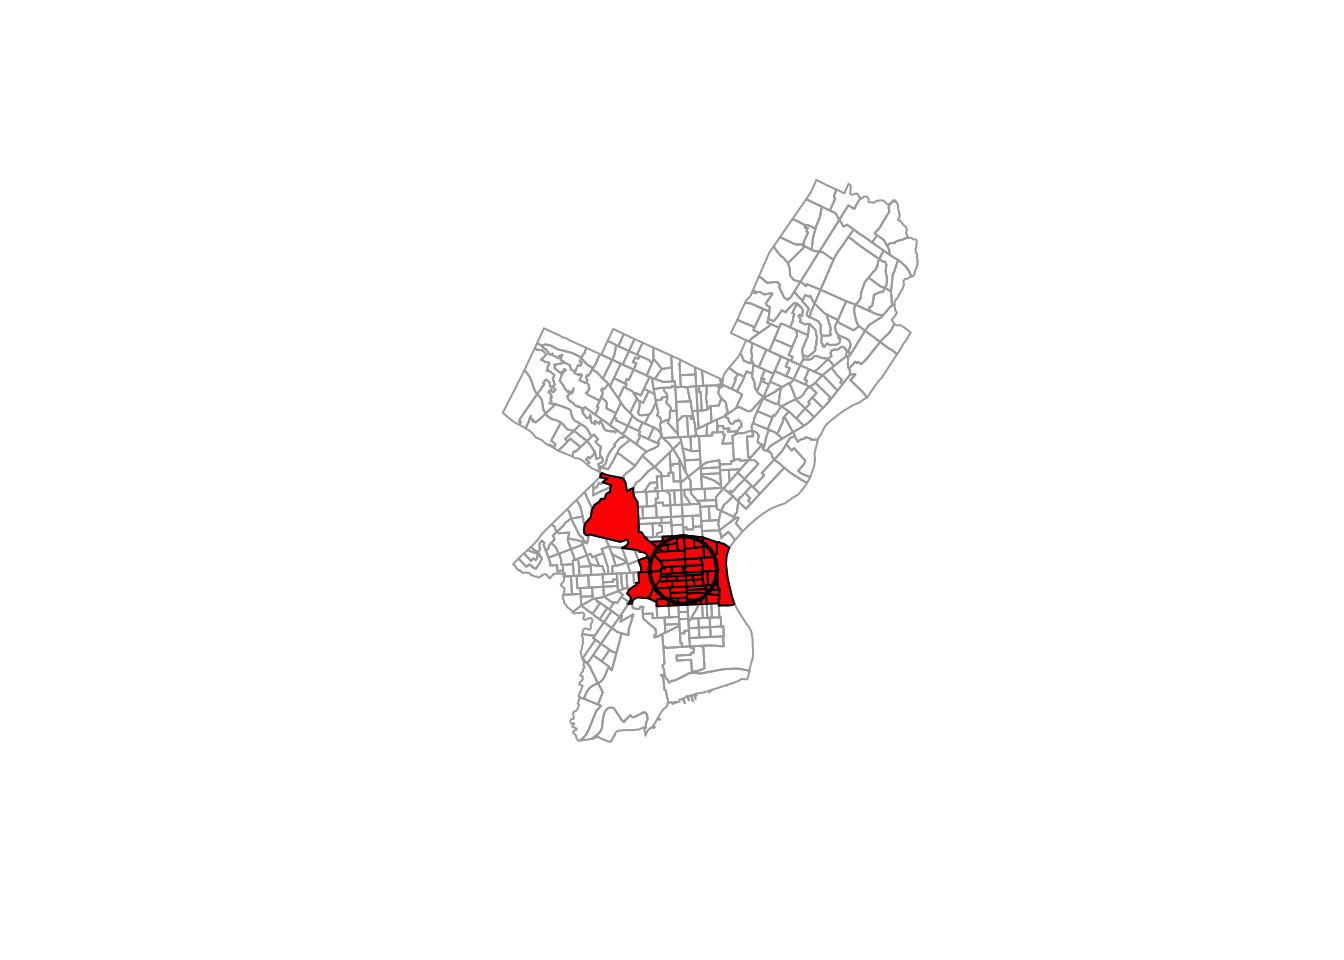
\includegraphics{R-spatial_files/figure-latex/sp-plot-selection-1.pdf}

\subsection{\texorpdfstring{Using the \texttt{sf}
package}{Using the sf package}}\label{using-the-sf-package}

To give you a sense of how this might be done using the \texttt{sf}
package we will reproduce here the same example as above.

For the spatial operations we can recur to the suite of geometric
operations that come with the \texttt{sf} package , in particular we
will use \texttt{st\_buffer()} and \texttt{st\_intersects()}

\begin{Shaded}
\begin{Highlighting}[]
\KeywordTok{library}\NormalTok{(sf)}
\NormalTok{philly_sf <-}\StringTok{ }\KeywordTok{st_read}\NormalTok{(}\StringTok{"data/Philly/"}\NormalTok{, }\DataTypeTok{quiet =}\NormalTok{ T)}

\CommentTok{# make a simple feature point with CRS}
\NormalTok{philly_ctr_sfc <-}\StringTok{ }\KeywordTok{st_sfc}\NormalTok{(}\KeywordTok{st_point}\NormalTok{(}\KeywordTok{c}\NormalTok{(}\OperatorTok{-}\FloatTok{75.16522}\NormalTok{, }\FloatTok{39.95258}\NormalTok{)), }\DataTypeTok{crs =} \DecValTok{4326}\NormalTok{)}

\CommentTok{# reproject}
\NormalTok{philly_ctr_aea_sf <-}\StringTok{ }\KeywordTok{st_transform}\NormalTok{(philly_ctr_sfc, }\KeywordTok{st_crs}\NormalTok{(philly_sf))}

\CommentTok{# create buffer}
\NormalTok{philly_buf_sf <-}\StringTok{ }\KeywordTok{st_buffer}\NormalTok{(philly_ctr_aea_sf, }\DecValTok{2000}\NormalTok{)}

\CommentTok{# find intersection between buffer and census polygons}
\NormalTok{philly_buf_intersects <-}\StringTok{ }\KeywordTok{st_intersects}\NormalTok{(philly_buf_sf, philly_sf)}
\KeywordTok{class}\NormalTok{(philly_buf_intersects)}
\end{Highlighting}
\end{Shaded}

\begin{verbatim}
#> [1] "sgbp"
\end{verbatim}

\begin{Shaded}
\begin{Highlighting}[]
\CommentTok{# subset}
\NormalTok{philly_sel_sf <-}\StringTok{ }\NormalTok{philly_sf[}\KeywordTok{unlist}\NormalTok{(philly_buf_intersects),]}

\CommentTok{# plot}
\KeywordTok{plot}\NormalTok{(}\KeywordTok{st_geometry}\NormalTok{(philly_sf), }\DataTypeTok{border=}\StringTok{"#aaaaaa"}\NormalTok{)}
\KeywordTok{plot}\NormalTok{(}\KeywordTok{st_geometry}\NormalTok{(philly_sel_sf), }\DataTypeTok{add=}\NormalTok{T, }\DataTypeTok{col=}\StringTok{"red"}\NormalTok{)}
\KeywordTok{plot}\NormalTok{(}\KeywordTok{st_geometry}\NormalTok{(philly_buf_sf), }\DataTypeTok{add=}\NormalTok{T, }\DataTypeTok{lwd =} \DecValTok{2}\NormalTok{)}
\end{Highlighting}
\end{Shaded}

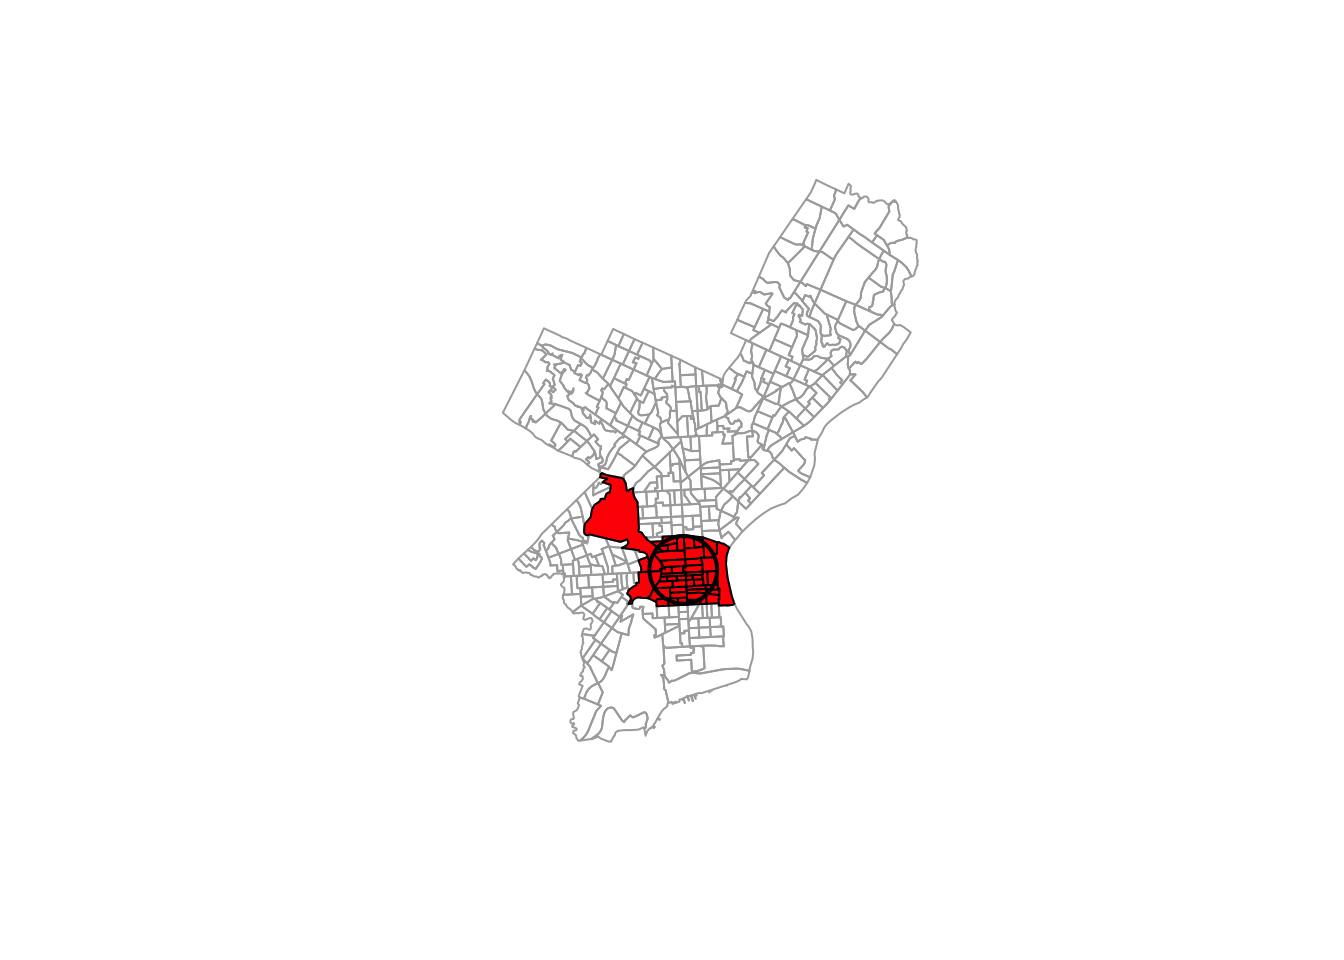
\includegraphics{R-spatial_files/figure-latex/sf-intersect-1.pdf}

\subsection{\texorpdfstring{\texttt{sp} - \texttt{sf}
comparison}{sp - sf comparison}}\label{sp---sf-comparison}

\begin{longtable}[]{@{}lll@{}}
\toprule
how to.. & for \texttt{sp} objects & for \texttt{sf}
objects\tabularnewline
\midrule
\endhead
join attributes & \texttt{sp::merge()} &
\texttt{base::merge()}\tabularnewline
reproject & \texttt{spTransform()} &
\texttt{st\_transform()}\tabularnewline
retrieve (or assign) CRS & \texttt{proj4string()} &
\texttt{st\_crs()}\tabularnewline
count points in polygons & \texttt{over()} & \texttt{st\_within} and
\texttt{aggregate()}\tabularnewline
buffer & \texttt{rgeos::gBuffer()} (separate package) &
\texttt{st\_buffer()}\tabularnewline
select by location &
\href{https://www.rdocumentation.org/packages/rgeos/}{\texttt{g*}
functions} from \texttt{rgeos} &
\href{https://www.rdocumentation.org/packages/sf/topics/geos}{geos
functions} in \texttt{sf}\tabularnewline
\bottomrule
\end{longtable}

\subsection{\texorpdfstring{\texttt{raster}
operations}{raster operations}}\label{raster-operations}

\begin{quote}
\begin{quote}
\begin{quote}
to come
\end{quote}
\end{quote}
\end{quote}

\chapter{Making Maps in R}\label{mapping}

\begin{quote}
Learning Objectives

\begin{itemize}
\tightlist
\item
  create a choropleth map with \texttt{spplot}
\item
  cprepare an \texttt{sp} object to be plotted with \texttt{ggplot}
\item
  create a choropleth map with \texttt{ggplot}
\item
  add a basemap with \texttt{ggmap}
\item
  use \texttt{RColorBrewer} to improve legend colors
\item
  use \texttt{classInt}to improve legend breaks
\item
  create a choropleth map with \texttt{tmap}
\item
  create an interactive map with \texttt{leaflet}
\item
  customize a \texttt{leaflet} map with popups and layer controls
\end{itemize}
\end{quote}

\begin{center}\rule{0.5\linewidth}{\linethickness}\end{center}

In the preceding examples we have used the base \texttt{plot} command to
take a quick look at our spatial objects.

In this section we will explore several alternatives to map spatial data
with R. For more packages see the ``Visualisation'' section of the
\href{https://cran.r-project.org/web/views/Spatial.html}{CRAN Task
View}.

Mapping packages are in the process of keeping up with the development
of the new \texttt{sf} package, so they typicall accept both \texttt{sp}
and \texttt{sf} objects. However, there are a few exceptions.

Of the packages shown here \texttt{spplot()}, which is part of the good
old \texttt{sp} package, only takes \texttt{sp} objects. The
\href{https://github.com/tidyverse/ggplot2/releases}{development version
of \texttt{ggplot2}} can take \texttt{sf} objects, though \texttt{ggmap}
\href{https://github.com/tidyverse/ggplot2/issues/2130}{seems to still
have issues} with \texttt{sf}. Both \texttt{tmap} and \texttt{leaflet}
can also handle both \texttt{sp} and \texttt{sf} objects.

\section{\texorpdfstring{Choropleth mapping with
\texttt{spplot}}{Choropleth mapping with spplot}}\label{choropleth-mapping-with-spplot}

\texttt{sp} comes with a plot command \texttt{spplot()}, which takes
\texttt{Spatial*} objects to plot. \texttt{spplot()} is one of the
earlier functions around to plot geographic objects.

We will use \texttt{readOGR()} from the \texttt{rgdal} libryary to read
back in the \texttt{PhillyCrimerate} shapefile we created earlyer back
into an object named \texttt{philly\_crimer\_sp}.

\begin{Shaded}
\begin{Highlighting}[]
\NormalTok{philly_crimer_sp <-}\StringTok{ }\KeywordTok{readOGR}\NormalTok{(}\StringTok{"data/PhillyCrimerate/"}\NormalTok{, }\StringTok{"PhillyCrimerate"}\NormalTok{, }\DataTypeTok{verbose =} \OtherTok{FALSE}\NormalTok{) }\CommentTok{# verbose = FALSE omits the output with the file info}
\KeywordTok{names}\NormalTok{(philly_crimer_sp)}
\end{Highlighting}
\end{Shaded}

\begin{verbatim}
#> [1] "OBJ_ID"     "homic_dens"
\end{verbatim}

By default \texttt{spplot} tries to map everything it can find in the
attribute table. Sometimes this does not work, depending on the data
types in the attribute table. The variables being compared must have a
range of values (or levels if they are factors). The following works,
but probably does not make too much sense:

\begin{Shaded}
\begin{Highlighting}[]
\KeywordTok{spplot}\NormalTok{(philly_crimer_sp)}
\end{Highlighting}
\end{Shaded}

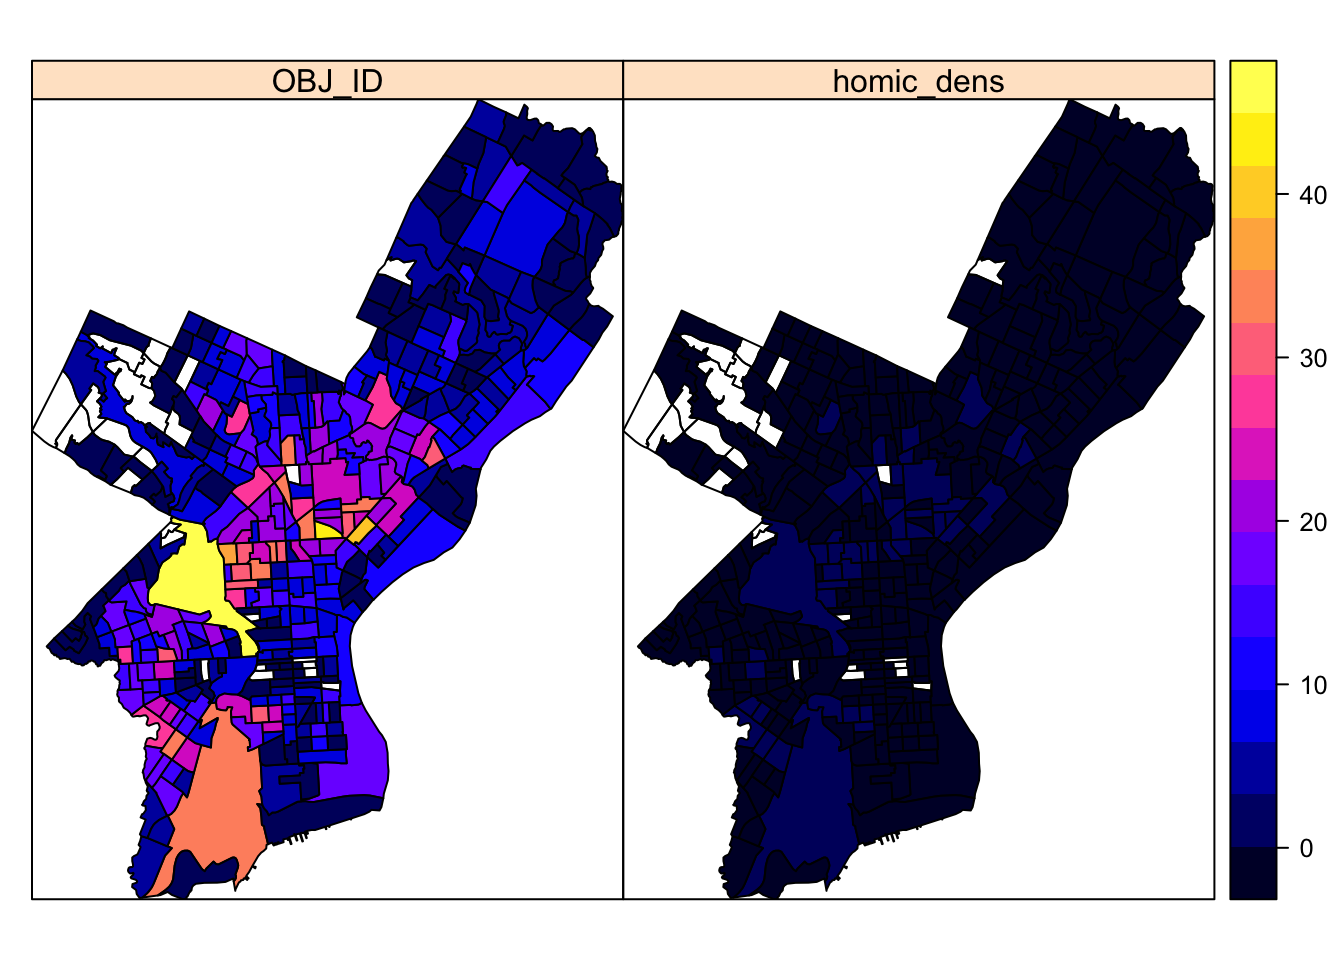
\includegraphics{R-spatial_files/figure-latex/spplot-default-1.pdf}

In order to select specific values to map we can provide the
\texttt{spplot} function with the name (or names) of the attribute
variable(s) we want to plot. It is the name of the column of the
\texttt{Spatial*Dataframe} as character string (or a vector if several).

\begin{Shaded}
\begin{Highlighting}[]
\KeywordTok{spplot}\NormalTok{(philly_crimer_sp, }\StringTok{"homic_dens"}\NormalTok{)}
\end{Highlighting}
\end{Shaded}

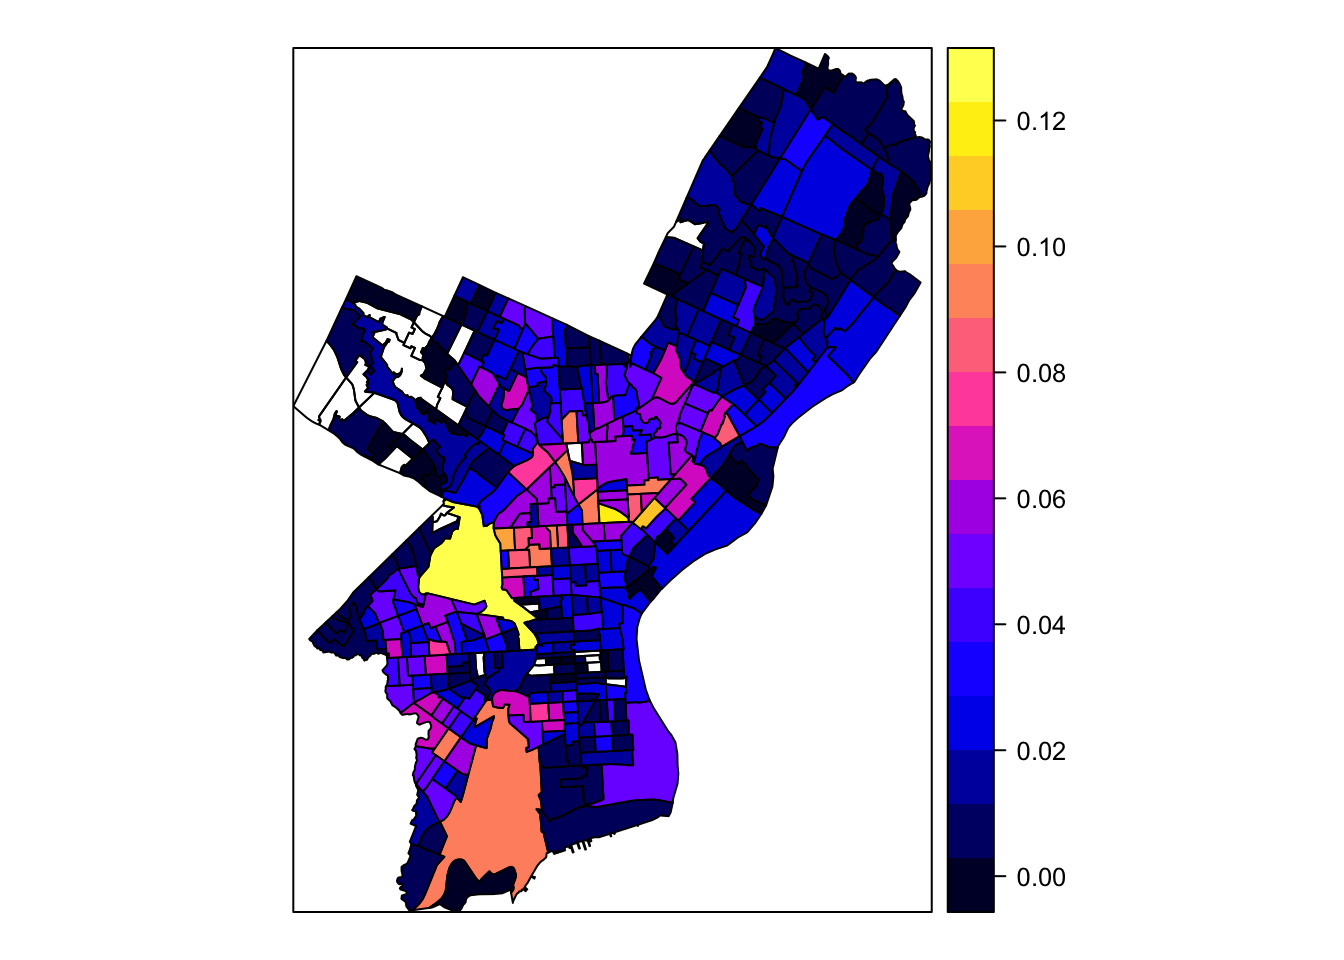
\includegraphics{R-spatial_files/figure-latex/spplot-single-1.pdf}

Let us try to improve this a little.

First off, we want to change the color palette. For this we use a
library called \texttt{RColorBrewer}\footnote{This is not the only way
  to provide color palettes. You can create your customized palette in
  many different ways or simply as a vector of hexbin color codes, like
  \texttt{c(\ "\#FDBB84"\ "\#FC8D59"\ "\#EF6548")}.}. For more about
ColorBrewer palettes read \href{http://colorbrewer2.org}{this}. Load the
\texttt{RColorBrewer} library and explore all sequential color schemes.

\begin{Shaded}
\begin{Highlighting}[]
\KeywordTok{library}\NormalTok{(RColorBrewer)}
\KeywordTok{display.brewer.all}\NormalTok{(}\DataTypeTok{type=}\StringTok{"seq"}\NormalTok{)}
\end{Highlighting}
\end{Shaded}

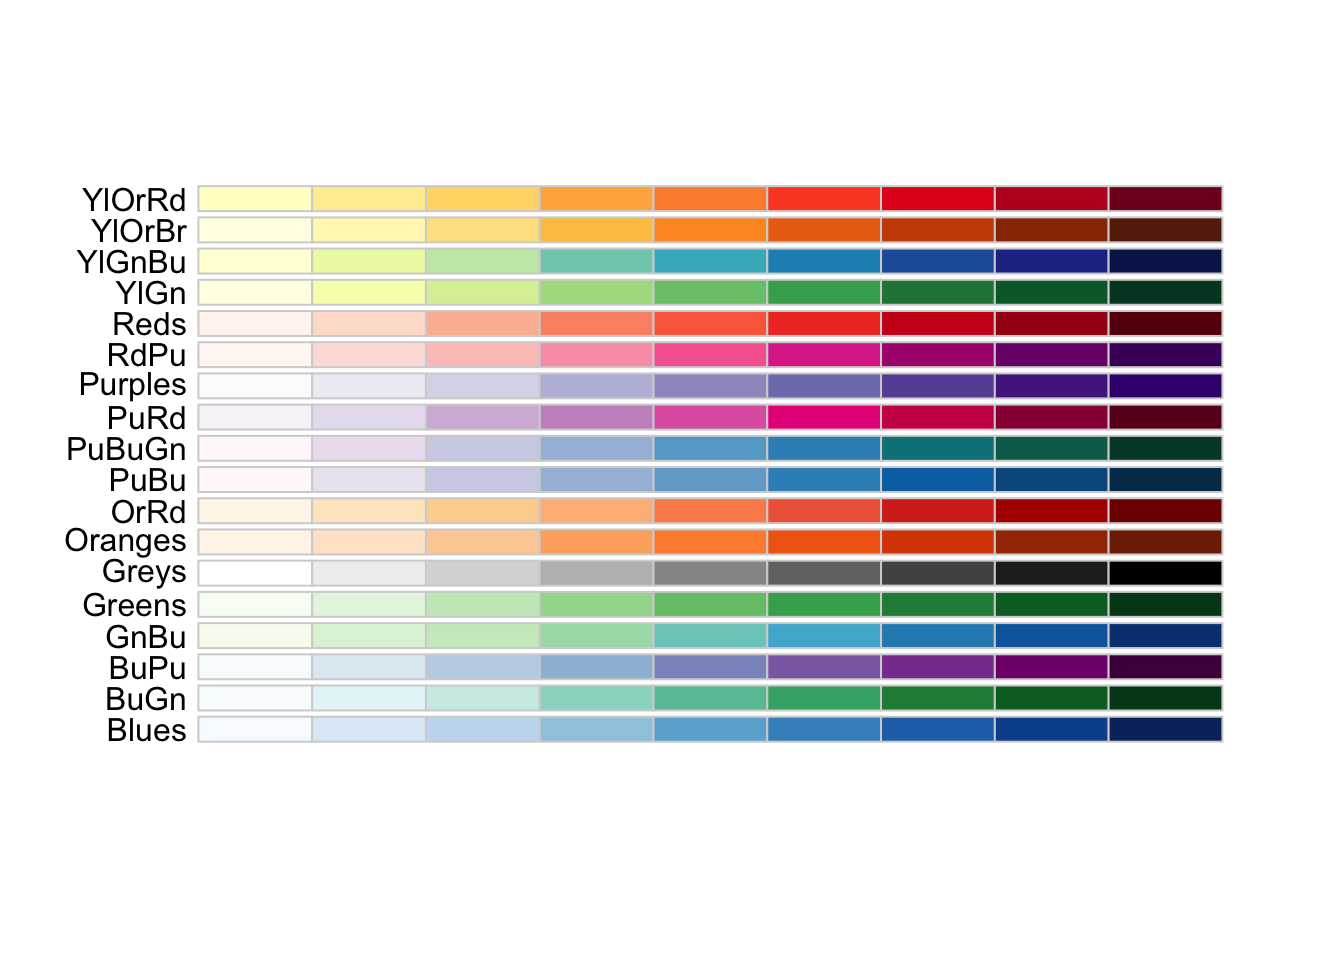
\includegraphics{R-spatial_files/figure-latex/colorbrewer-1.pdf}

To make the color palettes from ColorBrewer available as R palettes we
use the \texttt{brewer.pal()} funcdtion. It takes two arguments: - the
number of different colors desired and - the name of the palette as
character string.

We select 5 colors from the `Orange-Red' plaette and assign it to an
object \texttt{pal}.

\begin{Shaded}
\begin{Highlighting}[]
\NormalTok{pal <-}\StringTok{ }\KeywordTok{brewer.pal}\NormalTok{(}\DecValTok{5}\NormalTok{, }\StringTok{"OrRd"}\NormalTok{) }\CommentTok{# we select 5 colors from the palette}
\KeywordTok{class}\NormalTok{(pal)}
\end{Highlighting}
\end{Shaded}

\begin{verbatim}
#> [1] "character"
\end{verbatim}

Now we pass this information on to \texttt{spplot}. We need to provide
two more arguments:

\begin{itemize}
\tightlist
\item
  \texttt{col.regions} which we set to the palette we just created and
\item
  \texttt{cuts} which in our case is 4. It bins our continous variable
  into 5 brackets and will make our colors match up with those class
  brackets.
\end{itemize}

\begin{Shaded}
\begin{Highlighting}[]
\KeywordTok{spplot}\NormalTok{(philly_crimer_sp, }\StringTok{"homic_dens"}\NormalTok{, }\DataTypeTok{col.regions =}\NormalTok{ pal, }\DataTypeTok{cuts =} \DecValTok{4}\NormalTok{) }
\end{Highlighting}
\end{Shaded}

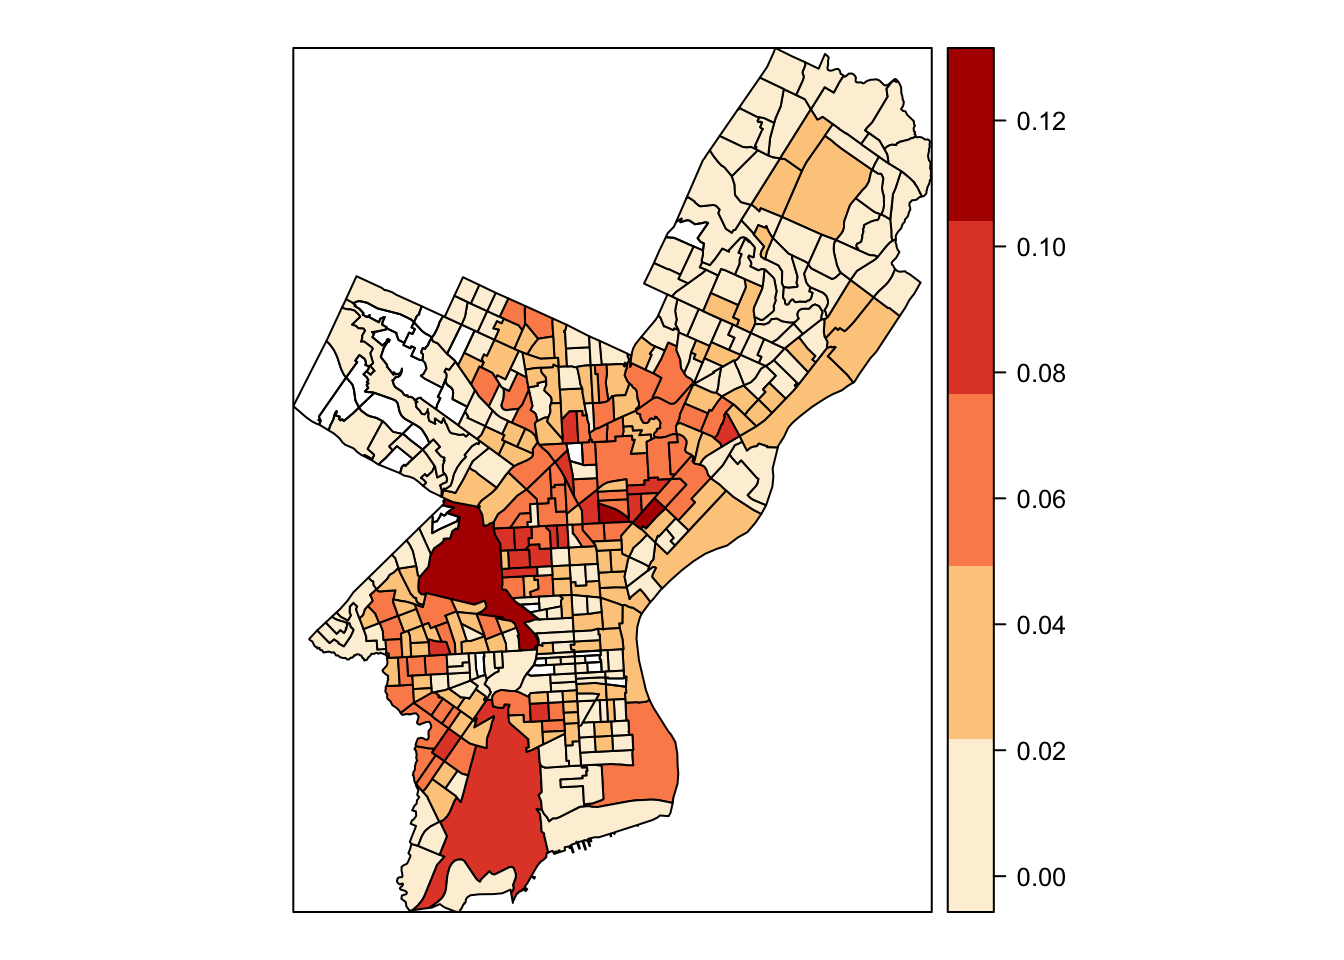
\includegraphics{R-spatial_files/figure-latex/spplot-palette-1.pdf}

Looks better already. However, since are unevenly distributed (see
below), in order to better distinguish the census tracts with low
values, we might want to set the breaks to quantiles.

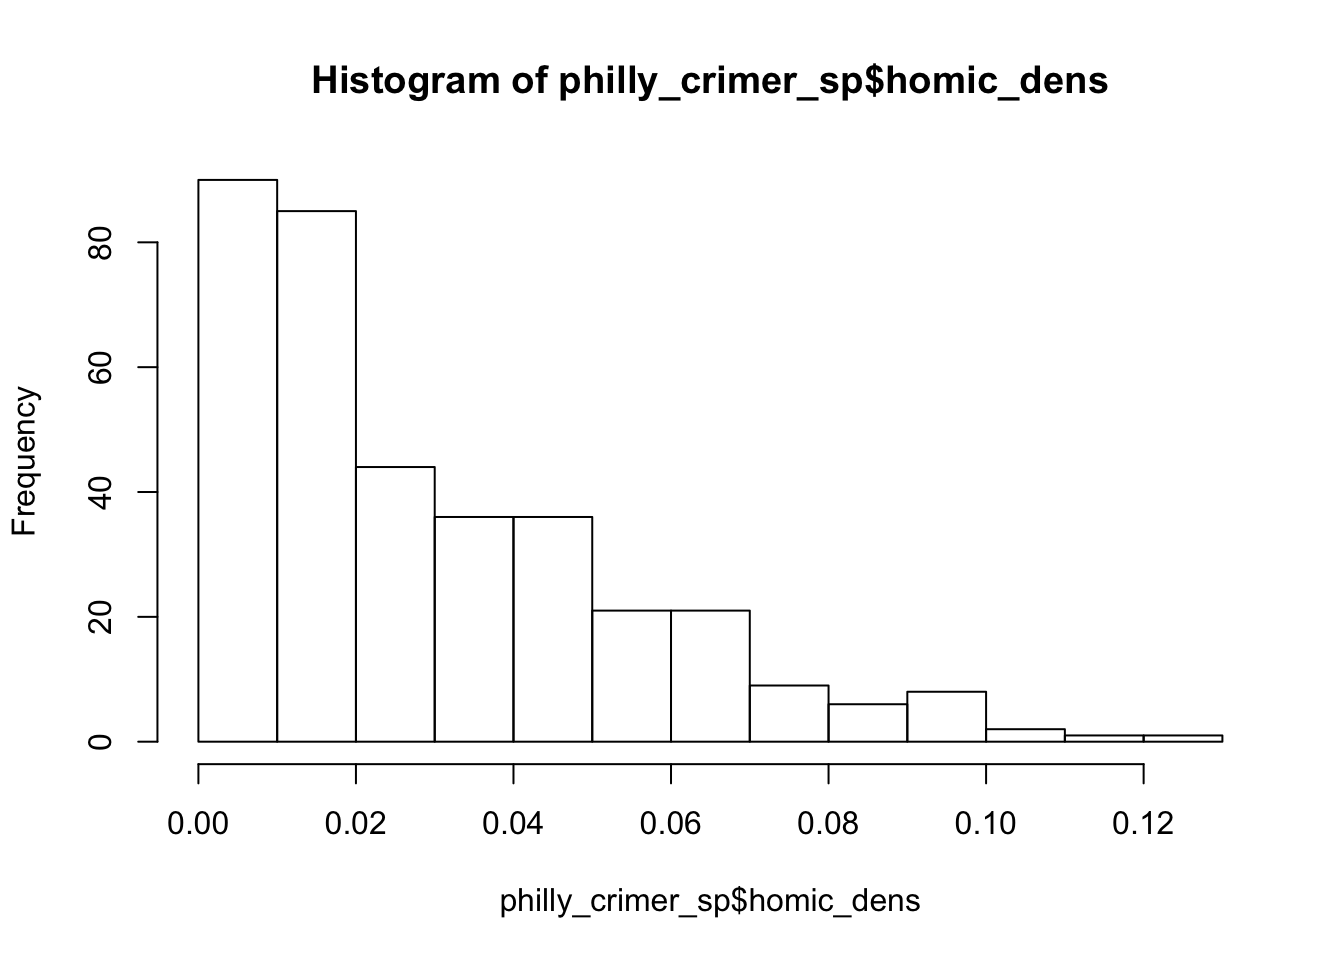
\includegraphics{R-spatial_files/figure-latex/unnamed-chunk-13-1.pdf}

We will use \texttt{classIntervals} from the \texttt{classInt} library.
This returns an object of type \texttt{classIntervals}, where we can
extract the values for the breaks. (Because of a the way spplot handles
break values\footnote{For the correction of breaks after using
  classIntervals with spplot/levelplot see here
  \url{http://r.789695.n4.nabble.com/SpatialPolygon-with-the-max-value-gets-no-color-assigned-in-spplot-function-when-using-quot-at-quot-r-td4654672.html}}
we need to shift them slightly.)

\begin{Shaded}
\begin{Highlighting}[]
\KeywordTok{library}\NormalTok{(classInt)}
\NormalTok{breaks_qt <-}\StringTok{ }\KeywordTok{classIntervals}\NormalTok{(philly_crimer_sp}\OperatorTok{$}\NormalTok{homic_dens, }\DataTypeTok{n =} \DecValTok{5}\NormalTok{, }\DataTypeTok{style =} \StringTok{"quantile"}\NormalTok{) }\CommentTok{# quantile is the default}
\end{Highlighting}
\end{Shaded}

\begin{verbatim}
#> Warning in classIntervals(philly_crimer_sp$homic_dens, n = 5, style =
#> "quantile"): var has missing values, omitted in finding classes
\end{verbatim}

\begin{Shaded}
\begin{Highlighting}[]
\KeywordTok{str}\NormalTok{(breaks_qt)  }\CommentTok{# structure of object}
\end{Highlighting}
\end{Shaded}

\begin{verbatim}
#> List of 2
#>  $ var : num [1:384] 0.00547 0.00821 0.03009 0.00821 0.01094 ...
#>  $ brks: num [1:6] 0.00274 0.00821 0.01641 0.02735 0.04923 ...
#>  - attr(*, "style")= chr "quantile"
#>  - attr(*, "nobs")= int 37
#>  - attr(*, "call")= language classIntervals(var = philly_crimer_sp$homic_dens, n = 5, style = "quantile")
#>  - attr(*, "intervalClosure")= chr "left"
#>  - attr(*, "class")= chr "classIntervals"
\end{verbatim}

\begin{Shaded}
\begin{Highlighting}[]
\NormalTok{breaks_qt}\OperatorTok{$}\NormalTok{brks  }\CommentTok{# break values}
\end{Highlighting}
\end{Shaded}

\begin{verbatim}
#> [1] 0.002735248 0.008205745 0.016411491 0.027352484 0.049234472 0.123086179
\end{verbatim}

\begin{Shaded}
\begin{Highlighting}[]
\CommentTok{# add a very small value to the top breakpoint, and subtract from the bottom for symmetry }
\NormalTok{br <-}\StringTok{ }\NormalTok{breaks_qt}\OperatorTok{$}\NormalTok{brks }
\NormalTok{offs <-}\StringTok{ }\FloatTok{0.0000001} 
\NormalTok{br[}\DecValTok{1}\NormalTok{] <-}\StringTok{ }\NormalTok{br[}\DecValTok{1}\NormalTok{] }\OperatorTok{-}\StringTok{ }\NormalTok{offs }
\NormalTok{br[}\KeywordTok{length}\NormalTok{(br)] <-}\StringTok{ }\NormalTok{br[}\KeywordTok{length}\NormalTok{(br)] }\OperatorTok{+}\StringTok{ }\NormalTok{offs }
\end{Highlighting}
\end{Shaded}

We use the breaks to set the \texttt{at=} argument in \texttt{spplot()}
and also set \texttt{main=} to add a title.

\begin{Shaded}
\begin{Highlighting}[]
\KeywordTok{spplot}\NormalTok{(philly_crimer_sp, }\StringTok{"homic_dens"}\NormalTok{, }\DataTypeTok{col.regions=}\NormalTok{pal, }\DataTypeTok{at=}\NormalTok{br,  }\DataTypeTok{main =} \StringTok{"Philadelphia homicide density per square km"}\NormalTok{)}
\end{Highlighting}
\end{Shaded}

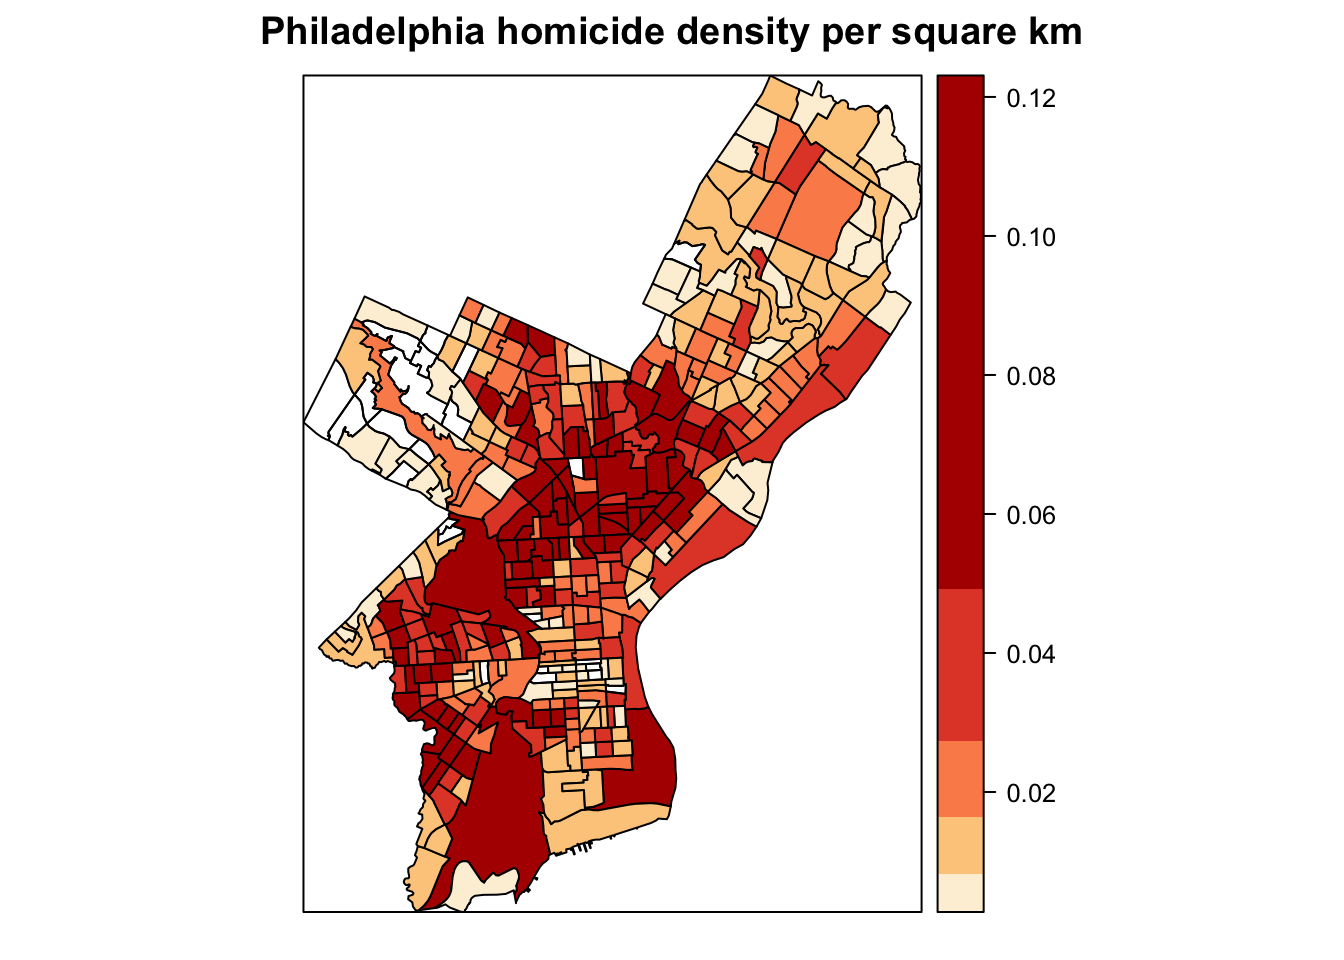
\includegraphics{R-spatial_files/figure-latex/spplot-breakds-corrected-1.pdf}

The final issue we will address is the legend, which shows as a
graduated color, since we provided a vector of continuous values to map.
Here is how we can change this:

\begin{itemize}
\tightlist
\item
  Use the \texttt{cut()} function from the base package with the values
  from \texttt{philly\_crimer\_sp\$homic\_dens} and the corrected breaks
  \texttt{br} to return a vector with the respective boundaries of the
  brackets. Use \texttt{?cut} if you need help.\\
\item
  Assign the output vector you get as a new column
  \texttt{homic\_dens\_bracket} to the \texttt{philly\_crimer\_sp}
  attributes table. It will help to map the color based on the breaks.
  Take a look at the values. What object class is that vector?\\
\item
  Remove the \texttt{at=} parameter in \texttt{spplot()} (which is only
  needed for continuous variables) and tell it to plot
  \texttt{homic\_dens\_bracket}.
\end{itemize}

\begin{Shaded}
\begin{Highlighting}[]
\NormalTok{philly_crimer_sp}\OperatorTok{$}\NormalTok{homic_dens_bracket <-}\StringTok{ }\KeywordTok{cut}\NormalTok{(philly_crimer_sp}\OperatorTok{$}\NormalTok{homic_dens, br)}
\KeywordTok{head}\NormalTok{(philly_crimer_sp}\OperatorTok{$}\NormalTok{homic_dens_bracket)}
\KeywordTok{class}\NormalTok{(philly_crimer_sp}\OperatorTok{$}\NormalTok{homic_dens_bracket)}
\KeywordTok{spplot}\NormalTok{(philly_crimer_sp, }\StringTok{"homic_dens_bracket"}\NormalTok{, }\DataTypeTok{col.regions=}\NormalTok{pal, }\DataTypeTok{main =} \StringTok{"Philadelphia homicide density per square km"}\NormalTok{)}
\end{Highlighting}
\end{Shaded}

Now, this is what you should see:

\begin{verbatim}
#> Warning in classIntervals(philly_crimer_sp$homic_dens, n = 5, style =
#> "quantile"): var has missing values, omitted in finding classes
\end{verbatim}

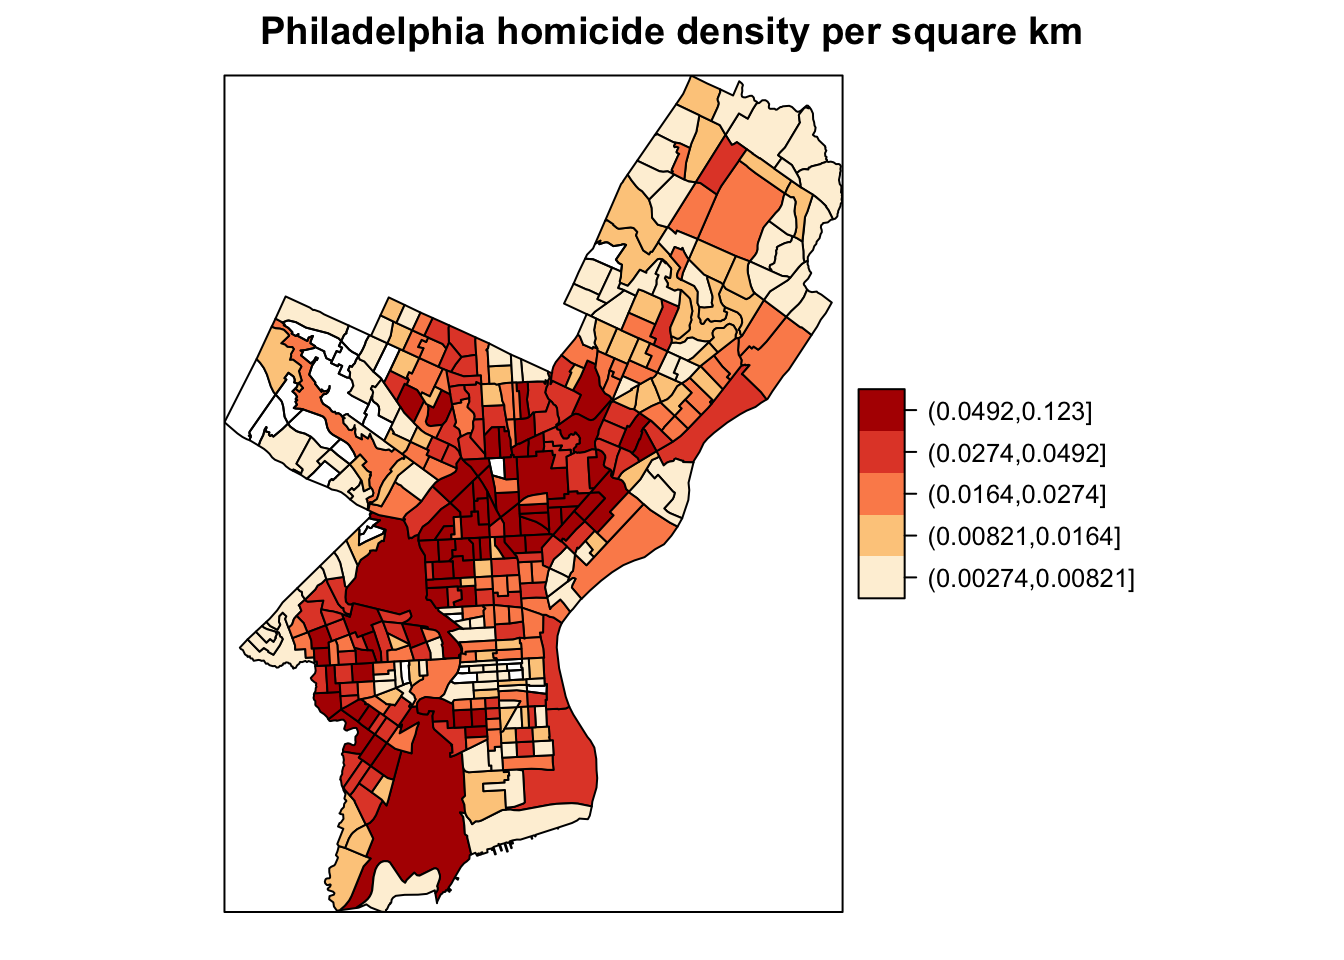
\includegraphics{R-spatial_files/figure-latex/spplot-final-map-1.pdf}

There are many more arguments for this function to provide additional
plot parameters, like the legend position, labels, scales, etc. but
we'll leave this for now.

\section{\texorpdfstring{Plotting simple features (\texttt{sf}) with
\texttt{plot}}{Plotting simple features (sf) with plot}}\label{plotting-simple-features-sf-with-plot}

The \texttt{sf} package extends the base \texttt{plot} command, so it
can be used on \texttt{sf} objects. If used without any arguments it
will plot all the attributes, like \texttt{spplot} does.

\begin{Shaded}
\begin{Highlighting}[]
\NormalTok{philly_crimer_sf <-}\StringTok{  }\KeywordTok{st_read}\NormalTok{(}\StringTok{"data/PhillyCrimerate/"}\NormalTok{)}
\end{Highlighting}
\end{Shaded}

\begin{verbatim}
#> Reading layer `PhillyCrimerate' from data source `/Users/cengel/Anthro/R_Class/R_Workshops/R-spatial/data/PhillyCrimerate' using driver `ESRI Shapefile'
#> Simple feature collection with 384 features and 2 fields
#> geometry type:  MULTIPOLYGON
#> dimension:      XY
#> bbox:           xmin: 1739497 ymin: 457343.7 xmax: 1764030 ymax: 490544.9
#> epsg (SRID):    NA
#> proj4string:    +proj=aea +lat_1=29.5 +lat_2=45.5 +lat_0=37.5 +lon_0=-96 +x_0=0 +y_0=0 +ellps=GRS80 +units=m +no_defs
\end{verbatim}

\begin{Shaded}
\begin{Highlighting}[]
\KeywordTok{plot}\NormalTok{(philly_crimer_sf)}
\end{Highlighting}
\end{Shaded}

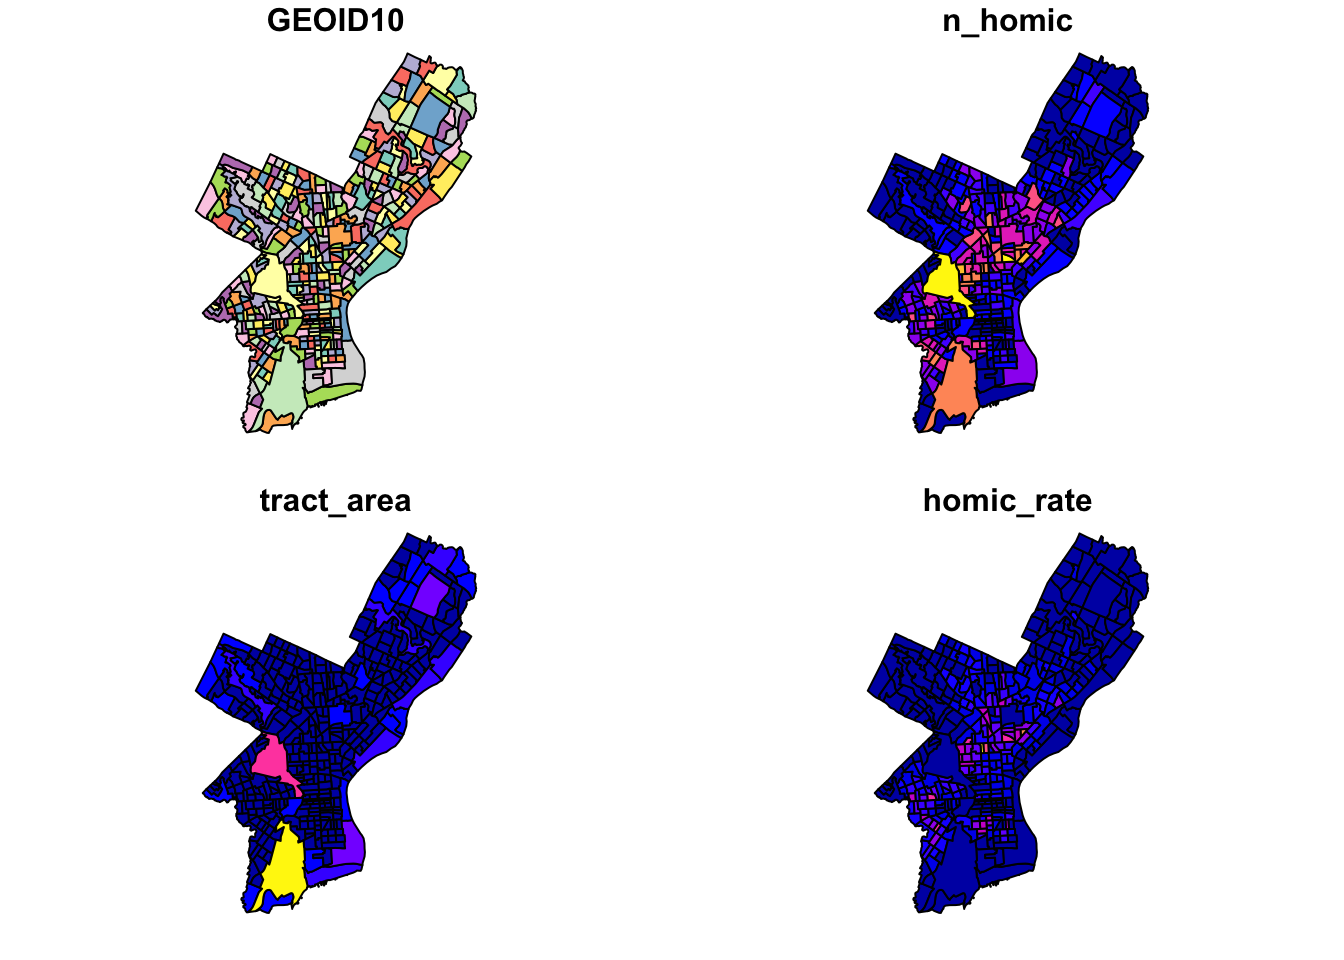
\includegraphics{R-spatial_files/figure-latex/sf-plot-default-1.pdf}

To plot a single attribute we need to provide an object of class
\texttt{sf}, like so:

\begin{Shaded}
\begin{Highlighting}[]
\KeywordTok{plot}\NormalTok{(philly_crimer_sf}\OperatorTok{$}\NormalTok{homic_dens) }\CommentTok{# this is a numeric vector!}
\end{Highlighting}
\end{Shaded}

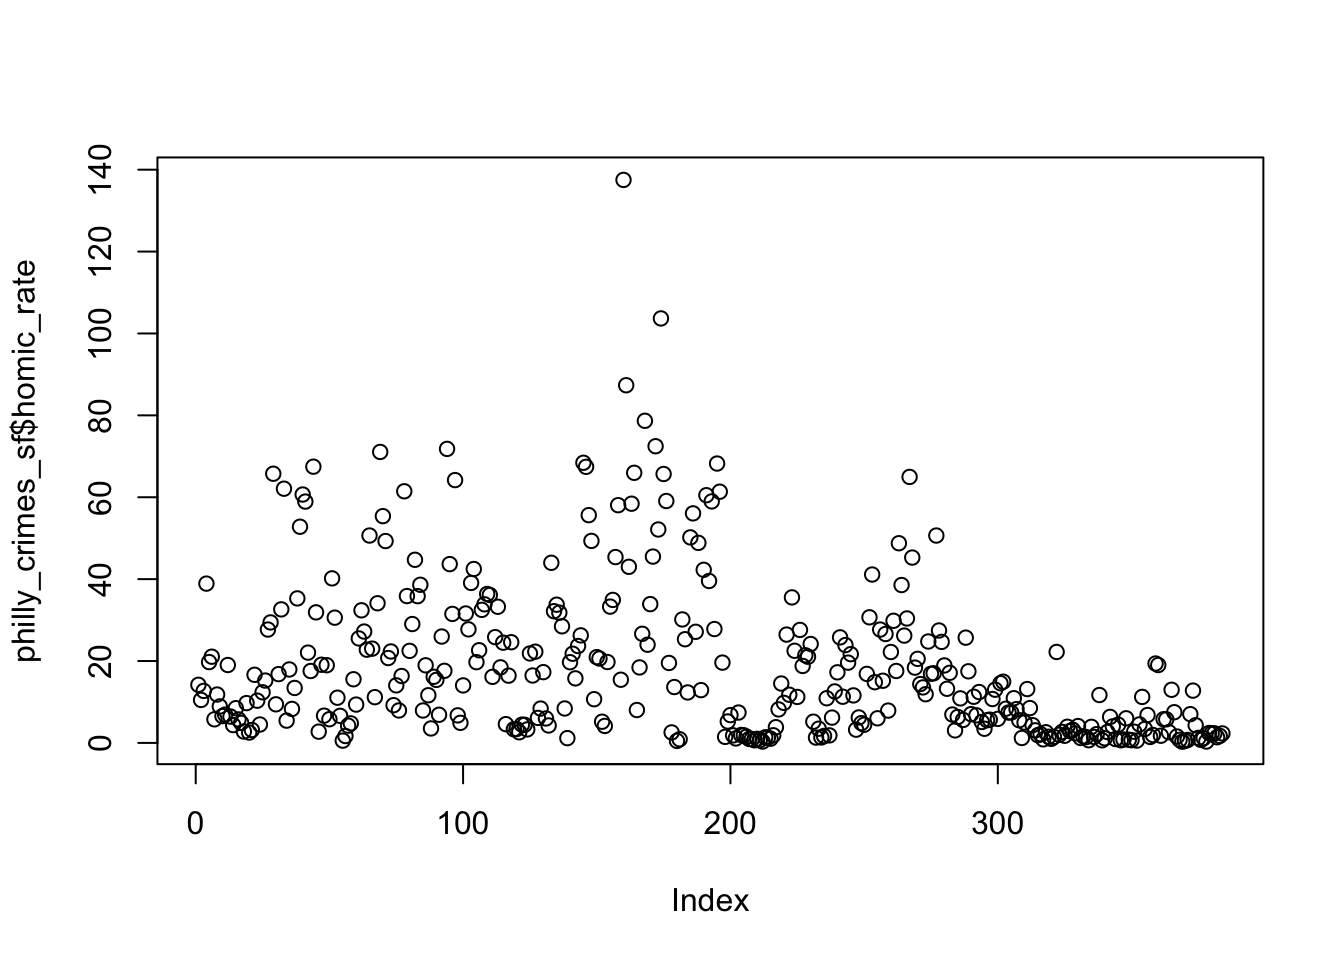
\includegraphics{R-spatial_files/figure-latex/sf-plot-single-1.pdf}

\begin{Shaded}
\begin{Highlighting}[]
\KeywordTok{plot}\NormalTok{(philly_crimer_sf[}\StringTok{"homic_dens"}\NormalTok{])}
\end{Highlighting}
\end{Shaded}

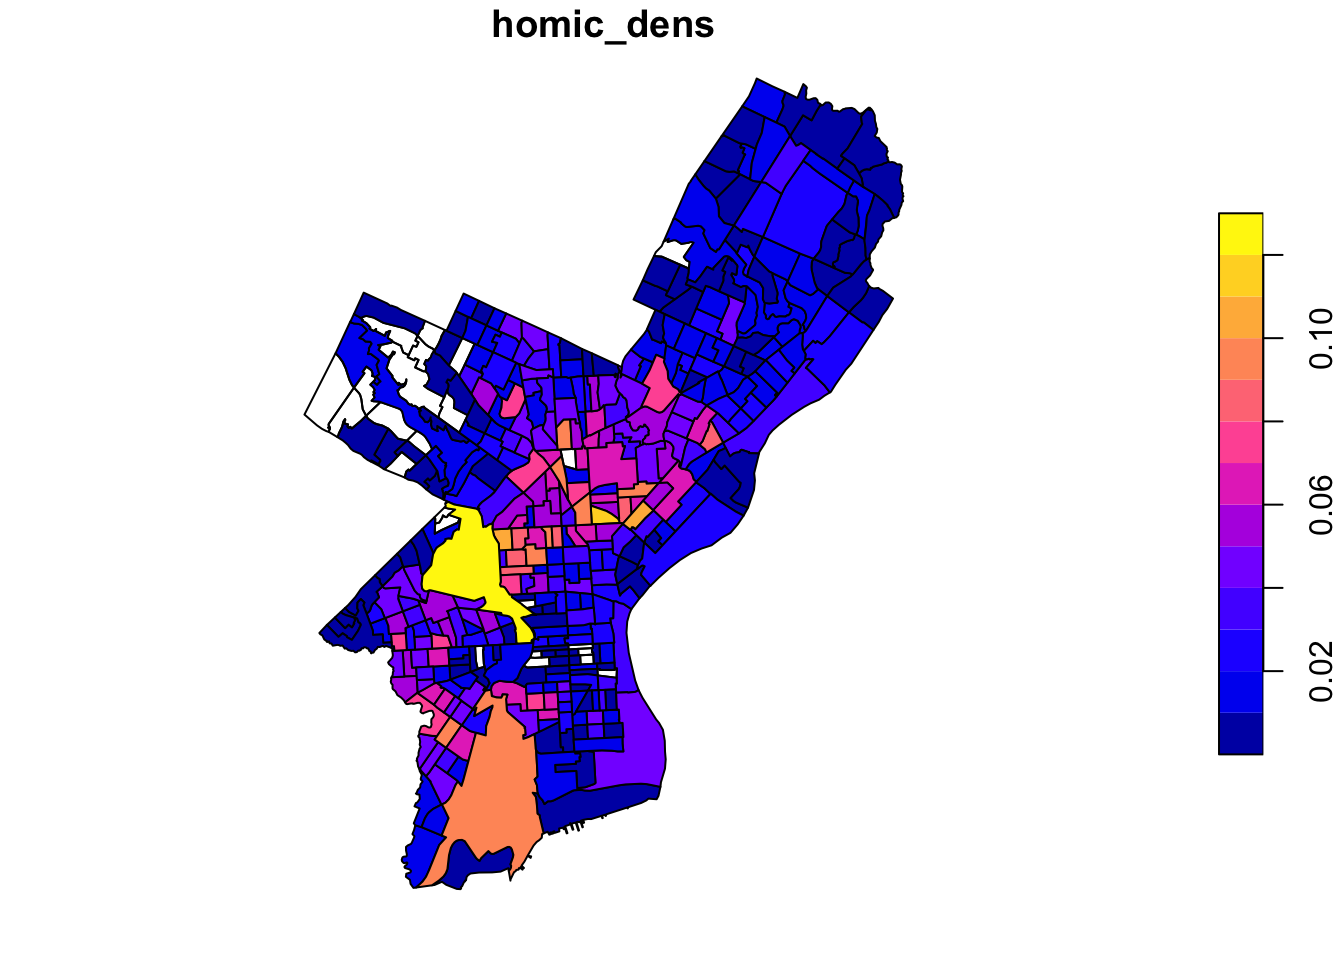
\includegraphics{R-spatial_files/figure-latex/sf-plot-single-2.pdf}

If we wanted to add our own colors, legend and title we would recur to
basic plot parameters to do this.

\begin{Shaded}
\begin{Highlighting}[]
\NormalTok{hr_cuts <-}\StringTok{ }\KeywordTok{cut}\NormalTok{(philly_crimer_sf}\OperatorTok{$}\NormalTok{homic_dens, br)}
\KeywordTok{plot}\NormalTok{(philly_crimer_sf[}\StringTok{"homic_dens"}\NormalTok{], }\DataTypeTok{main =} \StringTok{"Philadelphia homicide density per square km"}\NormalTok{, }\DataTypeTok{col =}\NormalTok{ pal[}\KeywordTok{as.numeric}\NormalTok{(hr_cuts)])}
\KeywordTok{legend}\NormalTok{(}\DecValTok{1760000}\NormalTok{, }\DecValTok{471000}\NormalTok{, }\DataTypeTok{legend =} \KeywordTok{paste}\NormalTok{(}\StringTok{"<"}\NormalTok{, }\KeywordTok{round}\NormalTok{(br[}\OperatorTok{-}\DecValTok{1}\NormalTok{])), }\DataTypeTok{fill =}\NormalTok{ pal)        }
\end{Highlighting}
\end{Shaded}

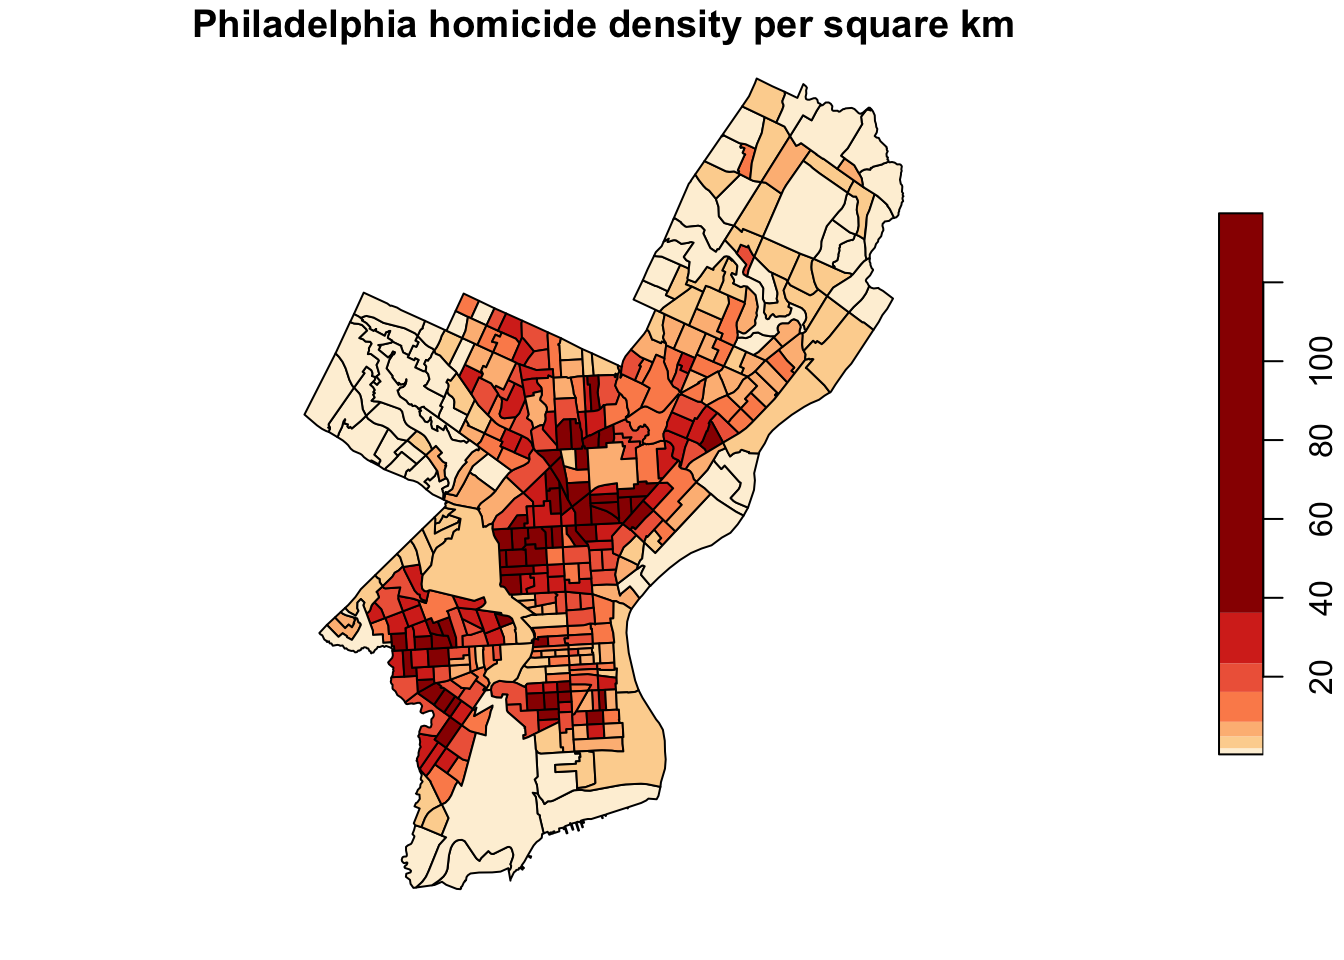
\includegraphics{R-spatial_files/figure-latex/sf-plot-legend-1.pdf}

\section{\texorpdfstring{Choropleth mapping with
\texttt{ggplot2}}{Choropleth mapping with ggplot2}}\label{choropleth-mapping-with-ggplot2}

\href{http://ggplot2.org/}{\texttt{ggplot2}} is a widely used and
powerful plotting library for R. It is not specifically geared towards
mapping, but one can generate great maps.

The \texttt{ggplot()} syntax is different from the previous as a plot is
built up by adding components with a \texttt{+}. You can start with a
layer showing the raw data then add layers of annotations and
statistical summaries. This allows to easily superimpose either
different visualizations of one dataset (e.g.~a scatterplot and a fitted
line) or different datasets (like different layers of the same
geographical area)\footnote{See Wilkinson L (2005): ``The grammar of
  graphics''. Statistics and computing, 2nd ed. Springer, New York.}.

For an introduction to \texttt{ggplot} check out
\href{http://link.springer.com/book/10.1007\%2F978-3-319-24277-4}{this
book by the package creator} or
\href{http://ggplot2.tidyverse.org/}{this} for more pointers.

In order to build a plot you start with initializing a ggplot object. In
order to do that \texttt{ggplot()} takes:

\begin{itemize}
\tightlist
\item
  a data argument usually a \textbf{dataframe} and
\item
  a mapping argument where x and y values to be plotted are supplied.
\end{itemize}

In addition, minimally a geometry to be used to determine how the values
should be displayed. This is to be added after an \texttt{+}.

\begin{verbatim}
ggplot(data = my_data_frame, mapping = aes(x = name_of_column_with_x_value, y = name_of_column_with_y_value)) +
  geom_point()
\end{verbatim}

Or shorter:

\begin{verbatim}
ggplot(my_data_frame, aes(name_of_column_with_x_value, name_of_column_with_y_value)) +
  geom_point()
\end{verbatim}

So if we wanted to map polygons, like census tract boundaries, we would
use longitude and latitude of their vertices as our \texttt{x} and
\texttt{y} values and \texttt{geom\_polygon()} as our geometry.

To plot the equivalent to the map we created with \texttt{spplot} above
we need to convert \texttt{philly\_crimer\_sp}, which is a
\texttt{SpatialPolygonsDataframe}, to a regular dataframe.
\texttt{broom} is a general purpose package which provides functions to
turn the messy output of built-in functions in R, such as lm, nls, or
t.test, into \href{https://www.jstatsoft.org/article/view/v059i10}{tidy
data} frames. We use the \texttt{tidy()} command for the
conversion\footnote{You may still see examples that use
  \texttt{ggplot2::fortify}. This will likely be deprecated in the
  future.}.

We use use the \texttt{tidy}function from the \texttt{broom} package for
the conversion and create a new object, \texttt{philly\_crimer\_df} for
the output.

\begin{Shaded}
\begin{Highlighting}[]
\KeywordTok{library}\NormalTok{(broom)}
\NormalTok{philly_crimer_df <-}\StringTok{ }\KeywordTok{tidy}\NormalTok{(philly_crimer_sp)}
\end{Highlighting}
\end{Shaded}

\begin{verbatim}
#> Regions defined for each Polygons
\end{verbatim}

\begin{Shaded}
\begin{Highlighting}[]
\KeywordTok{head}\NormalTok{(philly_crimer_df)}
\end{Highlighting}
\end{Shaded}

\begin{verbatim}
#>      long      lat order  hole piece group id
#> 1 1763647 484837.3     1 FALSE     1   0.1  0
#> 2 1763473 485194.5     2 FALSE     1   0.1  0
#> 3 1763366 485341.0     3 FALSE     1   0.1  0
#> 4 1763378 485353.9     4 FALSE     1   0.1  0
#> 5 1763321 485414.1     5 FALSE     1   0.1  0
#> 6 1762968 485731.8     6 FALSE     1   0.1  0
\end{verbatim}

Here are the important components of the output.

\begin{itemize}
\tightlist
\item
  \emph{long} and \emph{lat} of the vertices.
\item
  \emph{order.} This just shows in which order ggplot should ``connect
  the dots''
\item
  \emph{hole} Is this polygon a hole or not?
\item
  \emph{group.} This is very important! \texttt{geom\_} functions can
  take a group argument which controls (amongst other things) whether
  adjacent points should be connected by lines. If they are in the same
  group, then they get connected, but if they are in different groups
  then they don't. Essentially, having to points in different groups
  means that ggplot ``lifts the pen'' when going between them.
\end{itemize}

But wait. \texttt{tidy()} made us loose the attributes that we want to
map, so we have to take care of that. We extract the polygon IDs from
\texttt{philly\_crimer\_sp} and add them to its dataframe as a column,
named, for example, \texttt{polyID}. This requires a bit of
understanding of the internal structure of \texttt{philly\_crimer\_sp}.
You can take a peek with
\texttt{str(philly\_crimer\_sp,\ max.level\ =\ 2)}.

I use \texttt{slot(philly\_crimer\_sp,\ "polygons")} as argument to
\texttt{sapply()} to iterate over the polygons slots and then extract
the ID slot for each polygon, also with \texttt{slot()}.

Then we can use the polygon IDs with \texttt{merge()} to combine the
attribute table from \texttt{philly\_crimer\_sp} with
\texttt{philly\_crimer\_df}.

\begin{Shaded}
\begin{Highlighting}[]
\NormalTok{philly_crimer_sp}\OperatorTok{$}\NormalTok{polyID <-}\StringTok{ }
\StringTok{  }\KeywordTok{sapply}\NormalTok{(}\KeywordTok{slot}\NormalTok{(philly_crimer_sp, }\StringTok{"polygons"}\NormalTok{), }\ControlFlowTok{function}\NormalTok{(x) }\KeywordTok{slot}\NormalTok{(x, }\StringTok{"ID"}\NormalTok{))}
\NormalTok{philly_crimer_df <-}\StringTok{ }
\StringTok{  }\KeywordTok{merge}\NormalTok{(philly_crimer_df, philly_crimer_sp, }\DataTypeTok{by.x =} \StringTok{"id"}\NormalTok{, }\DataTypeTok{by.y=}\StringTok{"polyID"}\NormalTok{)}
\KeywordTok{head}\NormalTok{(philly_crimer_df)}
\end{Highlighting}
\end{Shaded}

\begin{verbatim}
#>   id    long      lat order  hole piece group OBJ_ID  homic_dens
#> 1  0 1763647 484837.3     1 FALSE     1   0.1      2 0.005470497
#> 2  0 1763473 485194.5     2 FALSE     1   0.1      2 0.005470497
#> 3  0 1763366 485341.0     3 FALSE     1   0.1      2 0.005470497
#> 4  0 1763378 485353.9     4 FALSE     1   0.1      2 0.005470497
#> 5  0 1763321 485414.1     5 FALSE     1   0.1      2 0.005470497
#> 6  0 1762968 485731.8     6 FALSE     1   0.1      2 0.005470497
#>   homic_dens_bracket
#> 1  (0.00274,0.00821]
#> 2  (0.00274,0.00821]
#> 3  (0.00274,0.00821]
#> 4  (0.00274,0.00821]
#> 5  (0.00274,0.00821]
#> 6  (0.00274,0.00821]
\end{verbatim}

OK. All set to plot.

There is a lot going on in this command, so I have provided comments in
the code.

\begin{Shaded}
\begin{Highlighting}[]
\KeywordTok{library}\NormalTok{(ggplot2)}

\KeywordTok{ggplot}\NormalTok{() }\OperatorTok{+}\StringTok{                                               }\CommentTok{# initialize ggplot object}
\StringTok{  }\KeywordTok{geom_polygon}\NormalTok{(                                          }\CommentTok{# make a polygon}
    \DataTypeTok{data =}\NormalTok{ philly_crimer_df,                             }\CommentTok{# data frame}
    \KeywordTok{aes}\NormalTok{(}\DataTypeTok{x =}\NormalTok{ long, }\DataTypeTok{y =}\NormalTok{ lat, }\DataTypeTok{group =}\NormalTok{ group,                }\CommentTok{# coordinates, and group them by polygons}
        \DataTypeTok{fill =} \KeywordTok{cut_number}\NormalTok{(homic_dens, }\DecValTok{5}\NormalTok{))) }\OperatorTok{+}\StringTok{                }\CommentTok{# variable to use for filling}
\StringTok{  }\KeywordTok{scale_fill_brewer}\NormalTok{(}\StringTok{"Density / sq km"}\NormalTok{, }\DataTypeTok{palette =} \StringTok{"OrRd"}\NormalTok{) }\OperatorTok{+}\StringTok{ }\CommentTok{# fill with brewer colors }
\StringTok{  }\KeywordTok{ggtitle}\NormalTok{(}\StringTok{"Philadelphia homicides"}\NormalTok{) }\OperatorTok{+}\StringTok{    }\CommentTok{# add title}
\StringTok{  }\KeywordTok{theme}\NormalTok{(}\DataTypeTok{line =} \KeywordTok{element_blank}\NormalTok{(),                          }\CommentTok{# remove axis lines .. }
        \DataTypeTok{axis.text=}\KeywordTok{element_blank}\NormalTok{(),                       }\CommentTok{# .. tickmarks..}
        \DataTypeTok{axis.title=}\KeywordTok{element_blank}\NormalTok{(),                      }\CommentTok{# .. axis labels..}
        \DataTypeTok{panel.background =} \KeywordTok{element_blank}\NormalTok{()) }\OperatorTok{+}\StringTok{            }\CommentTok{# .. background gridlines}
\StringTok{  }\KeywordTok{coord_equal}\NormalTok{()                                          }\CommentTok{# both axes the same scale}
\end{Highlighting}
\end{Shaded}

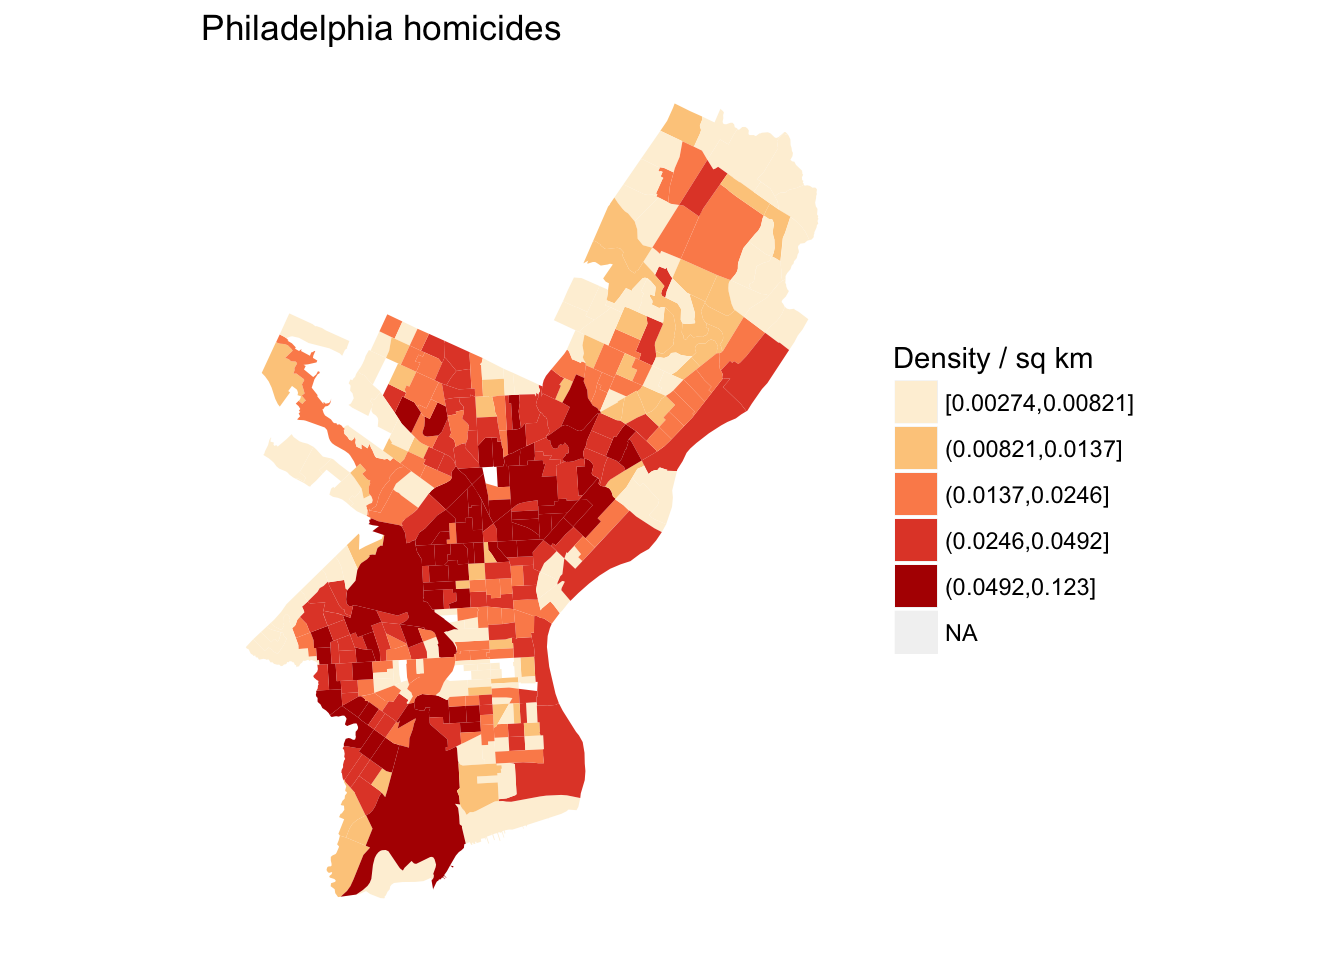
\includegraphics{R-spatial_files/figure-latex/ggplot-map-1.pdf}

\textbf{\texttt{ggplot} will soon be able to plot \texttt{sf} objects
directly.} This will look like:

\begin{verbatim}
ggplot(philly_sf) + geom_sf(aes(fill=homic_dens))
\end{verbatim}

\section{\texorpdfstring{Adding basemaps with
\texttt{ggmap}}{Adding basemaps with ggmap}}\label{adding-basemaps-with-ggmap}

\texttt{ggmap} builds on \texttt{ggplot} and allows to pull in tiled
basemaps from different services, like Google Maps and
OpenStreetMaps\footnote{Note that the use of Stamen Maps currently only
  works with a patch and that Cloudmade maps retired its API so it is no
  longer possible to be used as basemap.
  \href{https://CRAN.R-project.org/package=RgoogleMaps}{\texttt{RgoogleMaps}}
  is another library that provides an interface to query the Google
  server for static maps.}.

So let's overlay the map from above on a google satellite basemap.

First we use the \texttt{get\_map()} command from \texttt{ggmap} to pull
down the basemap. We need to tell it the location or the boundaries of
the map, the zoom level, and what kind of map service we like (default
is Google terrain). It will actually download the tile.
\texttt{get\_map()} returns a ggmap object, name it
\texttt{ph\_basemap}.

In order to view the map we then use \texttt{ggmap(ph\_basemap)}.

\begin{Shaded}
\begin{Highlighting}[]
\KeywordTok{library}\NormalTok{(ggmap)}

\CommentTok{# Philadelphia Lat 39.95258 and Lon is -75.16522}
\NormalTok{ph_basemap <-}\StringTok{ }\KeywordTok{get_map}\NormalTok{(}\DataTypeTok{location=}\KeywordTok{c}\NormalTok{(}\DataTypeTok{lon =} \OperatorTok{-}\FloatTok{75.16522}\NormalTok{, }\DataTypeTok{lat =} \FloatTok{39.95258}\NormalTok{), }\DataTypeTok{zoom=}\DecValTok{11}\NormalTok{, }\DataTypeTok{maptype =} \StringTok{'satellite'}\NormalTok{)}

\KeywordTok{ggmap}\NormalTok{(ph_basemap)}
\end{Highlighting}
\end{Shaded}

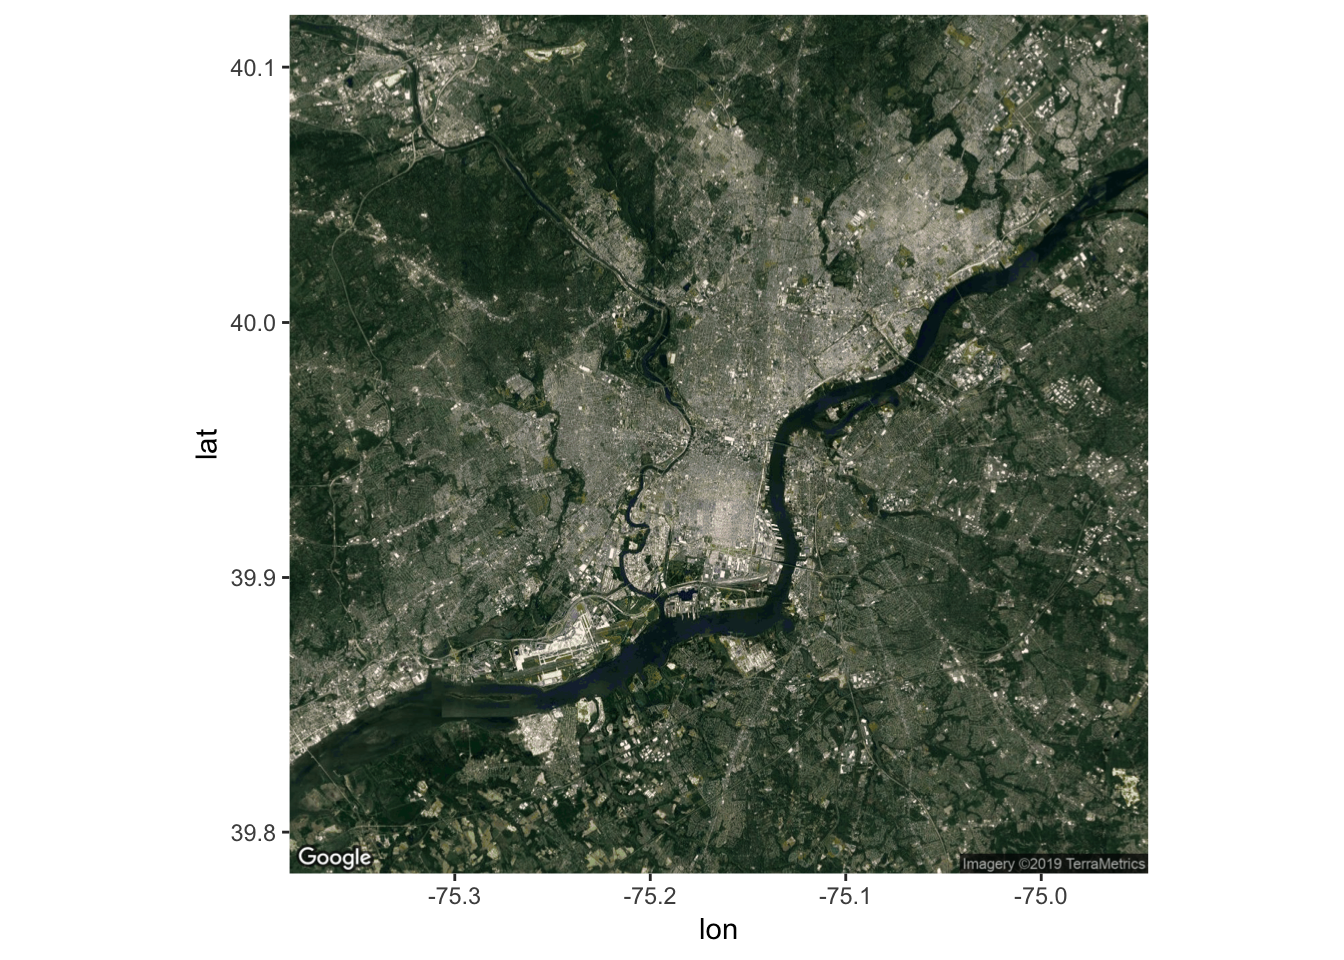
\includegraphics{R-spatial_files/figure-latex/ggmap-getmap-1.pdf}

Then we can reuse the code from the ggplot example above, just replacing
the first line, where we initialized a ggplot object above

\begin{verbatim}
    ggplot() + 
\end{verbatim}

with the line to call our basemap:

\begin{verbatim}
    ggmap(ph_basemap) +
\end{verbatim}

We also can get rid of the \texttt{theme()} and \texttt{coord\_equal()}
parts, as \texttt{ggmap} takes care of most of it.

\begin{Shaded}
\begin{Highlighting}[]
\KeywordTok{ggmap}\NormalTok{(ph_basemap) }\OperatorTok{+}
\StringTok{  }\KeywordTok{geom_polygon}\NormalTok{(}\DataTypeTok{data =}\NormalTok{ philly_crimer_df, }\KeywordTok{aes}\NormalTok{(}\DataTypeTok{x=}\NormalTok{long, lat, }\DataTypeTok{group =}\NormalTok{ group, }\DataTypeTok{fill =} \KeywordTok{cut_number}\NormalTok{(homic_dens, }\DecValTok{5}\NormalTok{))) }\OperatorTok{+}\StringTok{ }
\StringTok{  }\KeywordTok{scale_fill_brewer}\NormalTok{(}\StringTok{"Density / sq km"}\NormalTok{, }\DataTypeTok{palette =} \StringTok{"OrRd"}\NormalTok{) }\OperatorTok{+}\StringTok{ }
\StringTok{  }\KeywordTok{ggtitle}\NormalTok{(}\StringTok{"Philadelphia Homicides"}\NormalTok{) }
\end{Highlighting}
\end{Shaded}

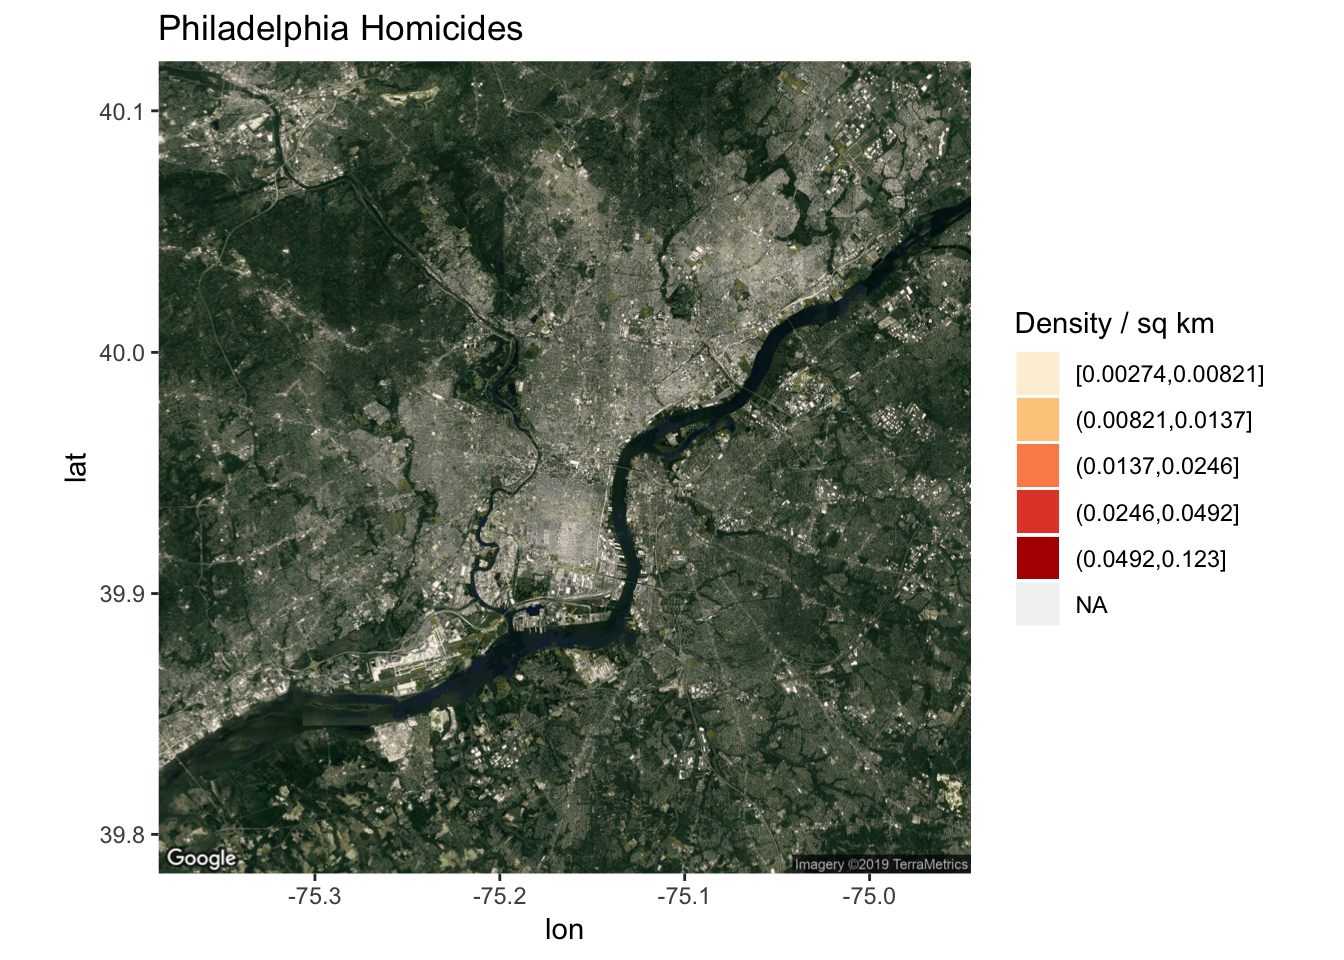
\includegraphics{R-spatial_files/figure-latex/ggmap-plot-misaligned-1.pdf}

Oops. Any idea what might be going on?

Unfortunately we have to go back to our original
\texttt{philly\_crimer\_sp} object and reproject it to the CRS (WGS84)
that works with Google maps. We then have to recreate our dataframe for
\texttt{ggplot}.

\begin{Shaded}
\begin{Highlighting}[]
\CommentTok{# reproject}
\NormalTok{philly_WGS84 <-}\StringTok{ }\KeywordTok{spTransform}\NormalTok{(philly_crimer_sp, }\KeywordTok{CRS}\NormalTok{(}\StringTok{"+init=epsg:4326"}\NormalTok{))}
\CommentTok{# create data frame}
\NormalTok{philly_df_WGS84 <-}\StringTok{ }\KeywordTok{tidy}\NormalTok{(philly_WGS84)}
\CommentTok{# add attribute data back in}
\NormalTok{philly_WGS84}\OperatorTok{$}\NormalTok{polyID <-}\StringTok{ }\KeywordTok{sapply}\NormalTok{(}\KeywordTok{slot}\NormalTok{(philly_WGS84, }\StringTok{"polygons"}\NormalTok{), }\ControlFlowTok{function}\NormalTok{(x) }\KeywordTok{slot}\NormalTok{(x, }\StringTok{"ID"}\NormalTok{))}
\NormalTok{philly_df_WGS84 <-}\StringTok{ }\KeywordTok{merge}\NormalTok{(philly_df_WGS84, philly_WGS84, }\DataTypeTok{by.x =} \StringTok{"id"}\NormalTok{, }\DataTypeTok{by.y=}\StringTok{"polyID"}\NormalTok{)}

\CommentTok{# plot}
\KeywordTok{ggmap}\NormalTok{(ph_basemap) }\OperatorTok{+}
\StringTok{  }\KeywordTok{geom_polygon}\NormalTok{(}\DataTypeTok{data =}\NormalTok{ philly_df_WGS84, }\KeywordTok{aes}\NormalTok{(}\DataTypeTok{x=}\NormalTok{long, lat, }\DataTypeTok{group =}\NormalTok{ group, }\DataTypeTok{fill =} \KeywordTok{cut_number}\NormalTok{(homic_dens, }\DecValTok{5}\NormalTok{)), }\DataTypeTok{alpha =} \FloatTok{0.8}\NormalTok{) }\OperatorTok{+}\StringTok{ }
\StringTok{  }\KeywordTok{scale_fill_brewer}\NormalTok{(}\StringTok{"Density / sq km"}\NormalTok{, }\DataTypeTok{palette =} \StringTok{"OrRd"}\NormalTok{) }\OperatorTok{+}\StringTok{ }
\StringTok{  }\KeywordTok{ggtitle}\NormalTok{(}\StringTok{"Philadelphia Homicides"}\NormalTok{)}
\end{Highlighting}
\end{Shaded}

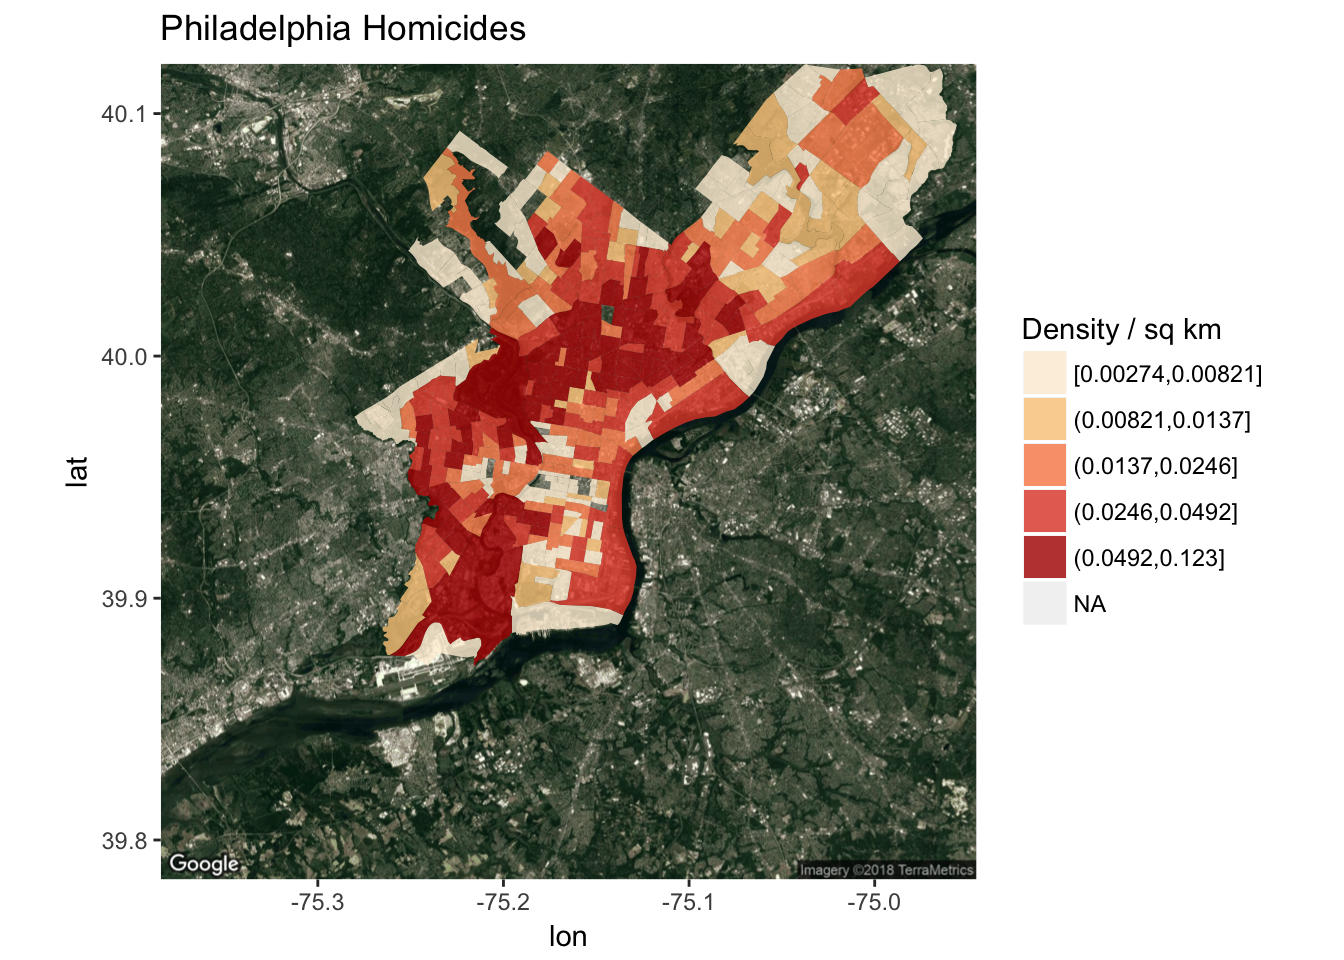
\includegraphics{R-spatial_files/figure-latex/ggmap-plot-aligned-1.pdf}

The \texttt{ggmap} package also includes functions for distance
calculations, geocoding, and calculating routes.

\section{\texorpdfstring{Choropleth with
\texttt{tmap}}{Choropleth with tmap}}\label{choropleth-with-tmap}

\texttt{tmap} is specifically designed to make creation of thematic maps
more convenient. It borrows from teh ggplot syntax and takes care of a
lot of the styling and aesthetics. This reduces our amount of code
significantly. We only need:

\begin{itemize}
\tightlist
\item
  \texttt{tm\_shape()} where we provide

  \begin{itemize}
  \tightlist
  \item
    the \texttt{SpatialPolygonsDataframe} (we could also provide an
    \texttt{sf} object)
  \end{itemize}
\item
  \texttt{tm\_polygons()} where we set

  \begin{itemize}
  \tightlist
  \item
    the attribute variable to map,
  \item
    the break style, and
  \item
    a title.
  \end{itemize}
\end{itemize}

\begin{Shaded}
\begin{Highlighting}[]
\KeywordTok{library}\NormalTok{(tmap)}
\KeywordTok{tm_shape}\NormalTok{(philly_crimer_sp) }\OperatorTok{+}
\StringTok{  }\KeywordTok{tm_polygons}\NormalTok{(}\StringTok{"homic_dens"}\NormalTok{, }
              \DataTypeTok{style=}\StringTok{"quantile"}\NormalTok{, }
              \DataTypeTok{title=}\StringTok{"Philadelphia }\CharTok{\textbackslash{}n}\StringTok{homicide density }\CharTok{\textbackslash{}n}\StringTok{per sqKm"}\NormalTok{)}
\end{Highlighting}
\end{Shaded}

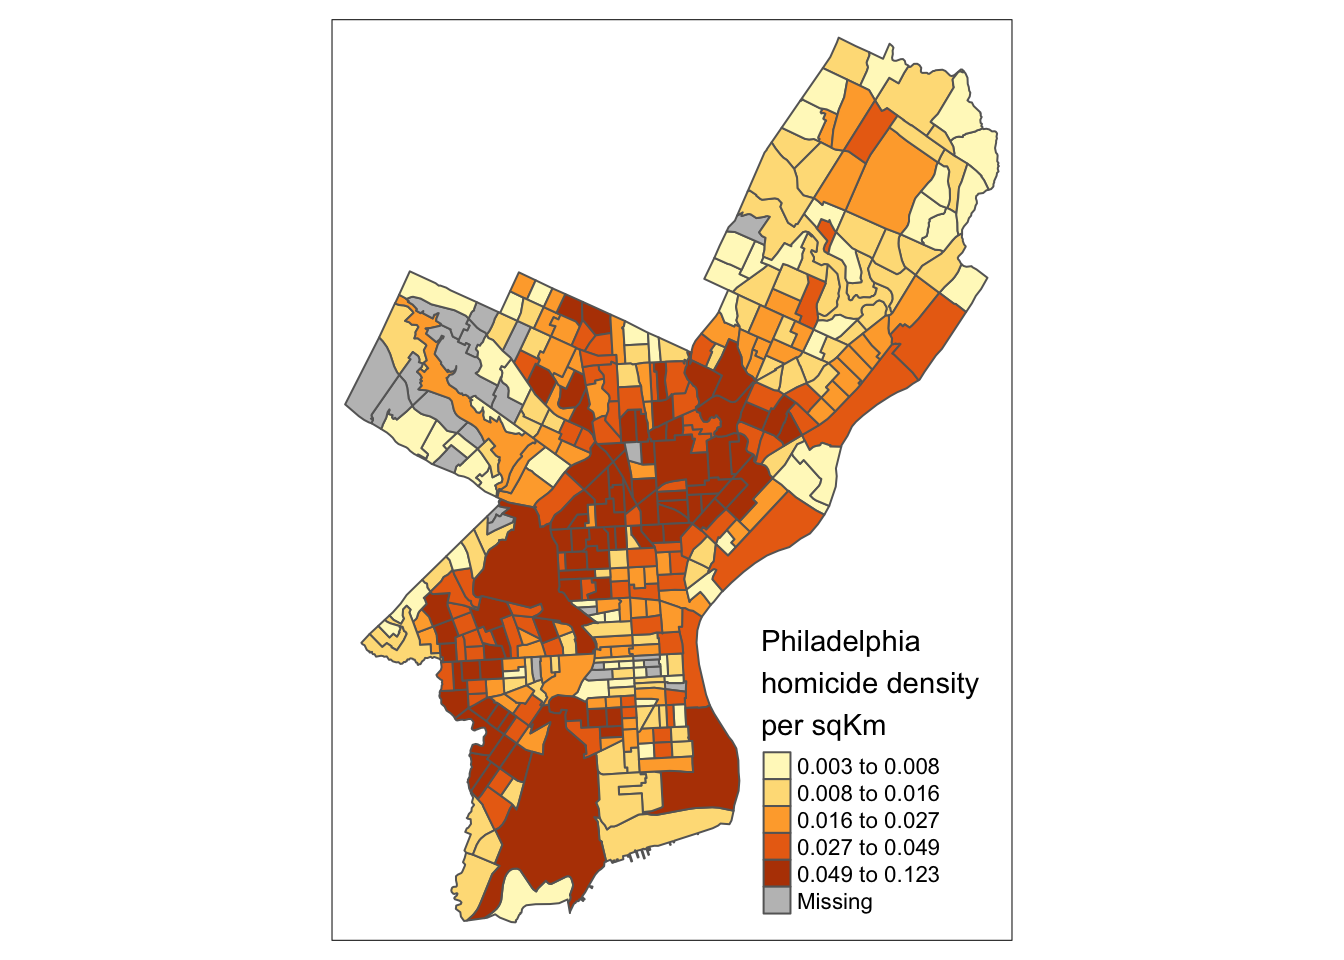
\includegraphics{R-spatial_files/figure-latex/tmap-plot-1.pdf}

\texttt{tmap} has a very nice feature that allows us to give basic
interactivity to the map. We can switch from ``plot'' mode into ``view''
mode and call the last plot, like so:

\begin{Shaded}
\begin{Highlighting}[]
\KeywordTok{tmap_mode}\NormalTok{(}\StringTok{"view"}\NormalTok{)}
\KeywordTok{last_map}\NormalTok{()}
\end{Highlighting}
\end{Shaded}

\includegraphics{R-spatial_files/figure-latex/tmap-plot-viewmode-1.pdf}

Cool huh?

The \texttt{tmap} library also includes functions for simple spatial
operations, geocoding and reverse geocoding using OSM. For more check
\texttt{vignette("tmap-nutshell")}.

\section{\texorpdfstring{Web mapping with
\texttt{leaflet}}{Web mapping with leaflet}}\label{web-mapping-with-leaflet}

\texttt{leaflet} provides bindings to the
\href{http://leafletjs.com}{`Leaflet' JavaScript library}, ``the leading
open-source JavaScript library for mobile-friendly interactive maps''.
We have already seen a simple use of leaflet in the \texttt{tmap}
example.

The good news is that the \texttt{leaflet} library gives us loads of
options to customize the web look and feel of the map.

The bad news is that the \texttt{leaflet} library gives us loads of
options to customize the web look and feel of the map.

Let's build up the map step by step.

First we load the \texttt{leaflet} library. Use the \texttt{leaflet()}
function with a \texttt{Spatial*} or \texttt{sp} object and pipe it to
\texttt{addPolygons()} function. It is not required, but improves
readability if you use \href{https://github.com/tidyverse/magrittr}{the
pipe operator \texttt{\%\textgreater{}\%}} to chain the elements
together when building up a map with \texttt{leaflet}.

\begin{Shaded}
\begin{Highlighting}[]
\KeywordTok{library}\NormalTok{(leaflet) }

\KeywordTok{leaflet}\NormalTok{(philly_WGS84) }\OperatorTok
\StringTok{  }\KeywordTok{addPolygons}\NormalTok{()}
\end{Highlighting}
\end{Shaded}

\includegraphics{R-spatial_files/figure-latex/leaflet-polys-1.pdf}

To map the homicide density we use \texttt{addPolygons()} and:

\begin{itemize}
\tightlist
\item
  remove stroke (polygon borders)\\
\item
  set a fillColor for each polygon based on \texttt{homic\_dens} and
  make it look nice by adjusting fillOpacity and smoothFactor (how much
  to simplify the polyline on each zoom level). The fill color is
  generated using \texttt{leaflet}'s \texttt{colorQuantile()} function,
  which takes the color scheme and the desired number of classes. To
  constuct the color scheme \texttt{colorQuantile()} returns a function
  that we supply to \texttt{addPolygons()} together with the name of the
  attribute variable to map.\\
\item
  add a popup with the \texttt{homic\_dens} values. We will create as a
  vector of strings, that we then supply to \texttt{addPolygons()}.
\end{itemize}

\begin{Shaded}
\begin{Highlighting}[]
\NormalTok{pal_fun <-}\StringTok{ }\KeywordTok{colorQuantile}\NormalTok{(}\StringTok{"YlOrRd"}\NormalTok{, }\OtherTok{NULL}\NormalTok{, }\DataTypeTok{n =} \DecValTok{5}\NormalTok{)}

\NormalTok{p_popup <-}\StringTok{ }\KeywordTok{paste0}\NormalTok{(}\StringTok{"<strong>Homicide Density: </strong>"}\NormalTok{, philly_WGS84}\OperatorTok{$}\NormalTok{homic_dens)}

\KeywordTok{leaflet}\NormalTok{(philly_WGS84) }\OperatorTok
\StringTok{  }\KeywordTok{addPolygons}\NormalTok{(}
    \DataTypeTok{stroke =} \OtherTok{FALSE}\NormalTok{, }\CommentTok{# remove polygon borders}
    \DataTypeTok{fillColor =} \OperatorTok{~}\KeywordTok{pal_fun}\NormalTok{(homic_dens), }\CommentTok{# set fill color with function from above and value}
    \DataTypeTok{fillOpacity =} \FloatTok{0.8}\NormalTok{, }\DataTypeTok{smoothFactor =} \FloatTok{0.5}\NormalTok{, }\CommentTok{# make it nicer}
    \DataTypeTok{popup =}\NormalTok{ p_popup)  }\CommentTok{# add popup}
\end{Highlighting}
\end{Shaded}

\includegraphics{R-spatial_files/figure-latex/leaflet-popups-1.pdf}

Here we add a basemap, which defaults to OSM, with \texttt{addTiles()}

\begin{Shaded}
\begin{Highlighting}[]
\KeywordTok{leaflet}\NormalTok{(philly_WGS84) }\OperatorTok
\StringTok{  }\KeywordTok{addPolygons}\NormalTok{(}
    \DataTypeTok{stroke =} \OtherTok{FALSE}\NormalTok{, }
    \DataTypeTok{fillColor =} \OperatorTok{~}\KeywordTok{pal_fun}\NormalTok{(homic_dens),}
    \DataTypeTok{fillOpacity =} \FloatTok{0.8}\NormalTok{, }\DataTypeTok{smoothFactor =} \FloatTok{0.5}\NormalTok{,}
    \DataTypeTok{popup =}\NormalTok{ p_popup) }\OperatorTok
\StringTok{  }\KeywordTok{addTiles}\NormalTok{()}
\end{Highlighting}
\end{Shaded}

\includegraphics{R-spatial_files/figure-latex/leaflet-basemap-1.pdf}

Lastly, we add a legend. We will provide the \texttt{addLegend()}
function with:

\begin{itemize}
\tightlist
\item
  the location of the legend on the map\\
\item
  the function that creates the color palette\\
\item
  the value we want the palette function to use\\
\item
  a title
\end{itemize}

\begin{Shaded}
\begin{Highlighting}[]
\KeywordTok{leaflet}\NormalTok{(philly_WGS84) }\OperatorTok
\StringTok{  }\KeywordTok{addPolygons}\NormalTok{(}
    \DataTypeTok{stroke =} \OtherTok{FALSE}\NormalTok{, }
    \DataTypeTok{fillColor =} \OperatorTok{~}\KeywordTok{pal_fun}\NormalTok{(homic_dens),}
    \DataTypeTok{fillOpacity =} \FloatTok{0.8}\NormalTok{, }\DataTypeTok{smoothFactor =} \FloatTok{0.5}\NormalTok{,}
    \DataTypeTok{popup =}\NormalTok{ p_popup) }\OperatorTok
\StringTok{  }\KeywordTok{addTiles}\NormalTok{() }\OperatorTok
\StringTok{  }\KeywordTok{addLegend}\NormalTok{(}\StringTok{"bottomright"}\NormalTok{,  }\CommentTok{# location}
            \DataTypeTok{pal=}\NormalTok{pal_fun,    }\CommentTok{# palette function}
            \DataTypeTok{values=}\OperatorTok{~}\NormalTok{homic_dens,  }\CommentTok{# value to be passed to palette function}
            \DataTypeTok{title =} \StringTok{'Philadelphia homicide density per sqkm'}\NormalTok{) }\CommentTok{# legend title}
\end{Highlighting}
\end{Shaded}

\includegraphics{R-spatial_files/figure-latex/leaflet-legend-1.pdf}

The labels of the legend show percentages instead of the actual value
breaks\footnote{The formatting is set with \texttt{labFormat()} and in
  the
  \href{https://cran.r-project.org/web/packages/leaflet/leaflet.pdf}{documentation}
  we discover that: ``By default, \texttt{labFormat} is basically
  \texttt{format(scientific\ =\ FALSE,big.mark\ =\ \textquotesingle{},\textquotesingle{})}
  for the numeric palette, \texttt{as.character()} for the factor
  palette, and a function to return labels of the form
  \texttt{x{[}i{]}\ -\ x{[}i\ +\ 1{]}} for bin and quantile palettes
  (\textbf{in the case of quantile palettes, x is the probabilities
  instead of the values of breaks}).''}.

To set the labels for our breaks manually we replace the \texttt{pal}
and \texttt{values} with the \texttt{colors} and \texttt{labels}
arguments and set those directly using \texttt{brewer.pal()} and
\texttt{breaks\_qt} from an earlier section above.

\begin{Shaded}
\begin{Highlighting}[]
\KeywordTok{leaflet}\NormalTok{(philly_WGS84) }\OperatorTok
\StringTok{  }\KeywordTok{addPolygons}\NormalTok{(}
    \DataTypeTok{stroke =} \OtherTok{FALSE}\NormalTok{, }
    \DataTypeTok{fillColor =} \OperatorTok{~}\KeywordTok{pal_fun}\NormalTok{(homic_dens),}
    \DataTypeTok{fillOpacity =} \FloatTok{0.8}\NormalTok{, }\DataTypeTok{smoothFactor =} \FloatTok{0.5}\NormalTok{,}
    \DataTypeTok{popup =}\NormalTok{ p_popup) }\OperatorTok
\StringTok{  }\KeywordTok{addTiles}\NormalTok{() }\OperatorTok
\StringTok{  }\KeywordTok{addLegend}\NormalTok{(}\StringTok{"bottomright"}\NormalTok{, }
            \DataTypeTok{colors =} \KeywordTok{brewer.pal}\NormalTok{(}\DecValTok{5}\NormalTok{, }\StringTok{"YlOrRd"}\NormalTok{), }
            \DataTypeTok{labels =} \KeywordTok{paste0}\NormalTok{(}\StringTok{"up to "}\NormalTok{, }\KeywordTok{format}\NormalTok{(breaks_qt}\OperatorTok{$}\NormalTok{brks[}\OperatorTok{-}\DecValTok{1}\NormalTok{], }\DataTypeTok{digits =} \DecValTok{2}\NormalTok{)),}
            \DataTypeTok{title =}  \StringTok{'Philadelphia homicide density per sqkm'}\NormalTok{)}
\end{Highlighting}
\end{Shaded}

\includegraphics{R-spatial_files/figure-latex/leaflet-labels-1.pdf}

That's more like it. Finally, I have added for you a control to switch
to another basemap and turn the philly polygon off and on. Take a look
at the changes in the code below.

\begin{Shaded}
\begin{Highlighting}[]
\KeywordTok{leaflet}\NormalTok{(philly_WGS84) }\OperatorTok
\StringTok{  }\KeywordTok{addPolygons}\NormalTok{(}
    \DataTypeTok{stroke =} \OtherTok{FALSE}\NormalTok{, }
    \DataTypeTok{fillColor =} \OperatorTok{~}\KeywordTok{pal_fun}\NormalTok{(homic_dens),}
    \DataTypeTok{fillOpacity =} \FloatTok{0.8}\NormalTok{, }\DataTypeTok{smoothFactor =} \FloatTok{0.5}\NormalTok{,}
    \DataTypeTok{popup =}\NormalTok{ p_popup,}
    \DataTypeTok{group =} \StringTok{"philly"}\NormalTok{) }\OperatorTok
\StringTok{  }\KeywordTok{addTiles}\NormalTok{(}\DataTypeTok{group =} \StringTok{"OSM"}\NormalTok{) }\OperatorTok
\StringTok{  }\KeywordTok{addProviderTiles}\NormalTok{(}\StringTok{"CartoDB.DarkMatter"}\NormalTok{, }\DataTypeTok{group =} \StringTok{"Carto"}\NormalTok{) }\OperatorTok
\StringTok{  }\KeywordTok{addLegend}\NormalTok{(}\StringTok{"bottomright"}\NormalTok{, }
            \DataTypeTok{colors =} \KeywordTok{brewer.pal}\NormalTok{(}\DecValTok{5}\NormalTok{, }\StringTok{"YlOrRd"}\NormalTok{), }
            \DataTypeTok{labels =} \KeywordTok{paste0}\NormalTok{(}\StringTok{"up to "}\NormalTok{, }\KeywordTok{format}\NormalTok{(breaks_qt}\OperatorTok{$}\NormalTok{brks[}\OperatorTok{-}\DecValTok{1}\NormalTok{], }\DataTypeTok{digits =} \DecValTok{2}\NormalTok{)),}
            \DataTypeTok{title =} \StringTok{'Philadelphia homicide density per sqkm'}\NormalTok{) }\OperatorTok
\StringTok{  }\KeywordTok{addLayersControl}\NormalTok{(}\DataTypeTok{baseGroups =} \KeywordTok{c}\NormalTok{(}\StringTok{"OSM"}\NormalTok{, }\StringTok{"Carto"}\NormalTok{), }
                   \DataTypeTok{overlayGroups =} \KeywordTok{c}\NormalTok{(}\StringTok{"philly"}\NormalTok{))  }
\end{Highlighting}
\end{Shaded}

\includegraphics{R-spatial_files/figure-latex/leaflet-control-1.pdf}

If you'd like to take this further here are a few pointers.

\begin{itemize}
\tightlist
\item
  \href{http://rstudio.github.io/leaflet/}{Leaflet for R}
\item
  \href{https://github.com/Robinlovelace/Creating-maps-in-R/blob/master/vignettes/vspd-base-shiny.Rmd}{Creating
  maps in R}
\item
  \href{https://cyberhelp.sesync.org/maps-in-R-lesson/}{Maps in R}
\end{itemize}

\href{https://cengel.shinyapps.io/RioSlaveMarket/}{Here is an example}
using \texttt{ggplot}, \texttt{leaflet}, \texttt{shiny}, and
\href{http://rmarkdown.rstudio.com/flexdashboard/}{RStudio's
flexdashboard} template to bring it all together.

Due to continous deleopment on this front the R mapping package
landscape is a bit volatile. Here are a few others, that I have come
across, but don't use.

An alternative you may want to be aware of the
\href{https://CRAN.R-project.org/package=GISTools}{\texttt{GISTools}}
package. It has not been updated for a while, but it can be quite
convenient for choropleth plotting. It's \texttt{choropleth()} function
is a convenience functions that wraps around \texttt{spplot()} Currently
\texttt{GISTools} cannot understand \texttt{sf} objects.

The
\href{https://CRAN.R-project.org/package=leafletR}{\texttt{leafletR}}
package does similar things, but requires the spatial object to be in
GeoJSON/TopoJSON format. It also has not been updated for a while. My
reason for using \texttt{leaflet} is that it integrates well with
RStudio, Shiny, and R Markdown and can take \texttt{sf} objects.

\bibliography{book.bib,packages.bib}


\end{document}
